\documentclass[12pt,onecolumn]{article}
\usepackage[utf8]{inputenc} % UTF8 input encoding
\usepackage[T2A]{fontenc}   % T2A font encoding for Cyrillic script
\usepackage[russian]{babel} % Russian language support
\usepackage{listings}
\usepackage{float}
\usepackage{mathtools}
\everymath{\displaystyle}
\usepackage{listings} 
\usepackage[usenames]{color}
\usepackage{hyperref}
\usepackage{geometry}
\usepackage{verbatim}
\usepackage{amsmath}
\newcommand{\nparagraph}[1]{\paragraph{#1}\mbox{}\\}
\geometry{
  a4paper,
  top=20mm, 
  right=20mm, 
  bottom=20mm, 
  left=25mm
}

\begin{document}
\setcounter{tocdepth}{4}
\begin{center}
    Федеральное государственное автономное образовательное учреждение высшего образования "Национальный Исследовательский Университет ИТМО"\\ 
    Мегафакультет Компьютерных Технологий и Управления\\
    Факультет Программной Инженерии и Компьютерной Техники \\
    
\includegraphics[scale=0.3]{image/itmo.jpg} % нужно закинуть картинку логтипа в папку с отчетом
\end{center}
\vspace{1cm}


\begin{center}
    \large \textbf{Вариант №2}\\
    \textbf{Лабораторная работа 1}\\
    по дисциплине\\
    \textbf{'Функциональная схемотехника'}
\end{center}

\vspace{2cm}

\begin{flushright}
  Выполнил Студент  группы P33102\\
  \textbf{Лапин Алексей Александрович}\\
  Преподаватель: \\
  \textbf{Васильев С.Е.}\\
\end{flushright}

\vspace{9cm}
\begin{center}
    г. Санкт-Петербург\\
    2024г.
\end{center}
\pagestyle{empty}

\newpage
\tableofcontents
\newpage
\pagestyle{plain}
\section{Цели работы:}
\begin{enumerate}
    \item Получить базовые знания о принципах построения цифровых интегральных схем с использованием технологии КМОП.
    \item Познакомиться с технологией SPICE-моделирования схем на транзисторах.
    \item Получить навыки описания схем базовых операционных элементов (БОЭ) комбинационного типа на вентильном уровне с использованием языка описания аппаратуры Verilog HDL.
\end{enumerate}
\section{Задание}
Лабораторная работа состоит из двух частей.

Первая часть посвящена проектированию цифровых вентилей на полевых транзисторах, построению схем на базе вентилей и знакомству с технологией SPICEмоделирования. Первая часть работы выполняется в программном пакете LTspice. При построении схем вентилей необходимо использовать КМОП-транзисторы с параметрами из файла, предоставленного преподавателем (см. раздел «Основы работы в среде LTspice»).

Вторая часть посвящена знакомству с языком описания аппаратуры Verilog HDL, изучению особенностей его использования для описания схем на вентильном уровне и приобретению навыков тестирования таких схем. Вторая часть работы выполняется с использованием Vivado Simulator, входящего в пакет Vivado Design Suite (см. раздел «Основы работы в среде Vivado Design Suite»).

\textbf{Вариант}: 2

\textbf{Логический базис}: NAND

\textbf{БОЭ}: Полный четырехразрядный компаратор

\section{Отчет о выполнении заданий части 1:}
\subsection{Схема разработанного вентиля NAND}
\begin{figure}[H]
    \centering
    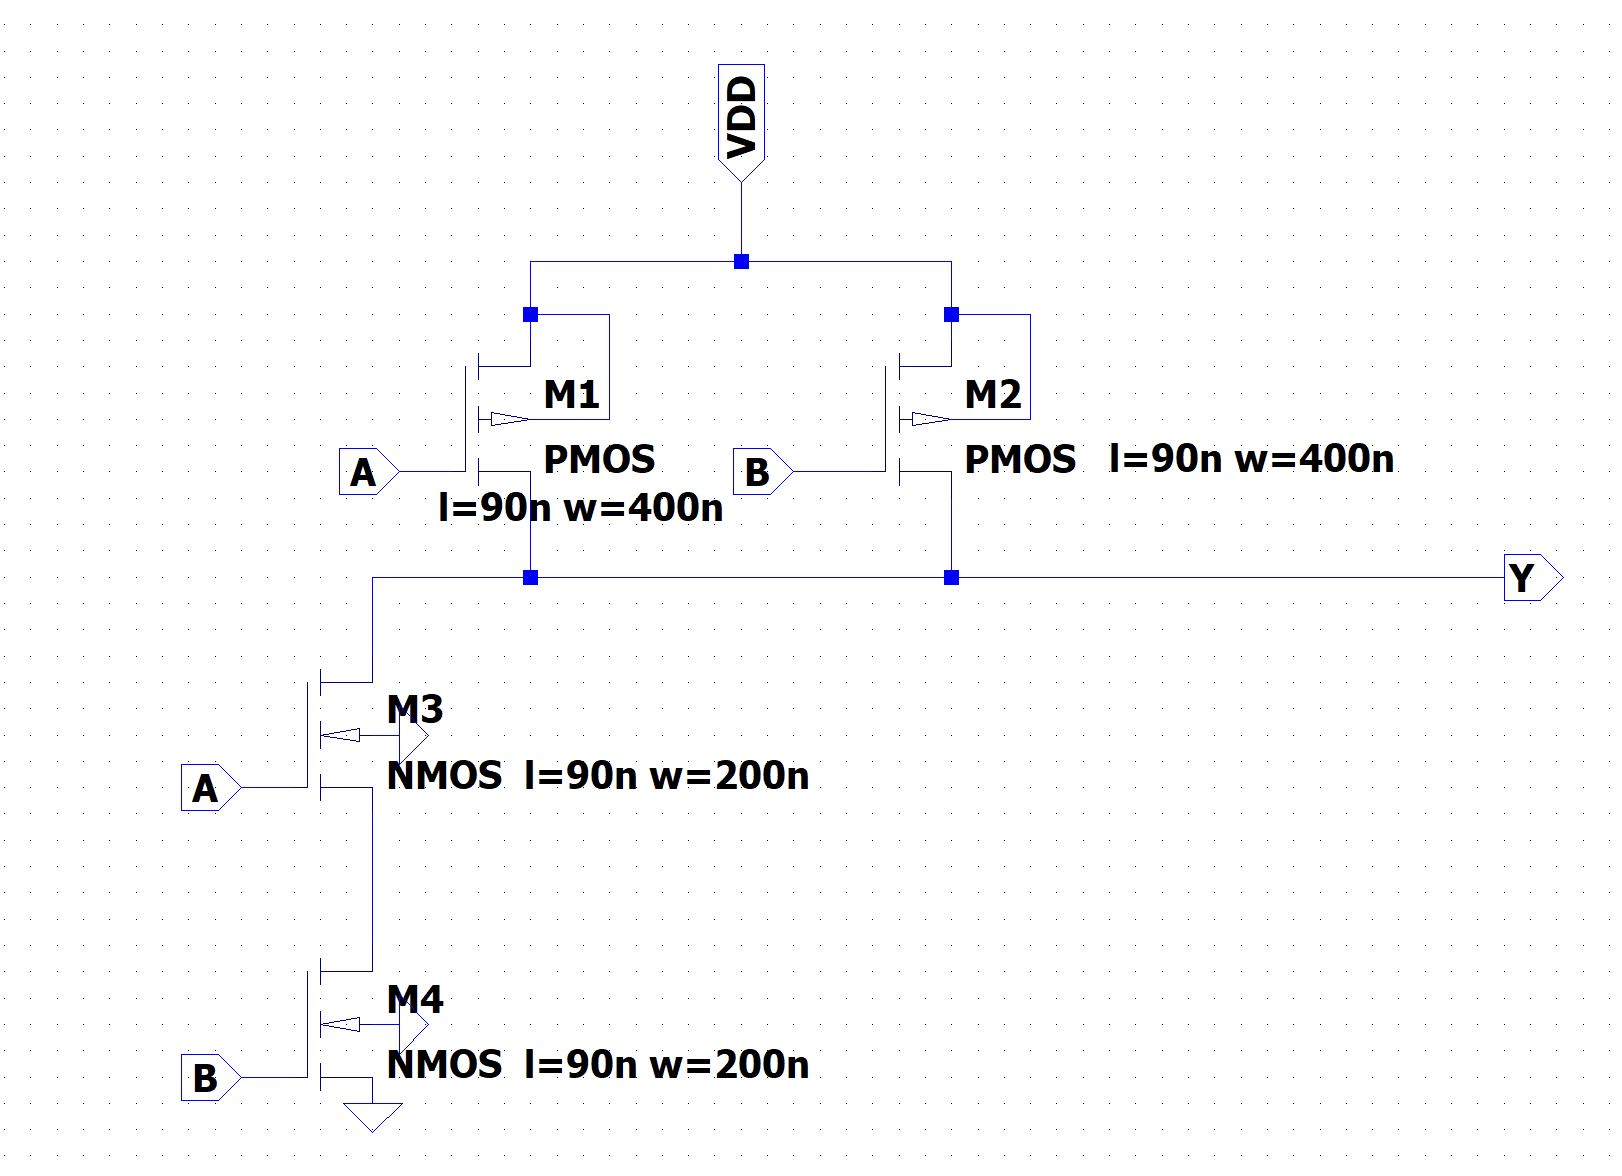
\includegraphics[scale=0.5]{image/ventil.png}
    \caption{Схема разработанного вентиля NAND}
\end{figure}
\subsection{Символ вентиля и схема тестирования}
\begin{figure}[H]
    \centering
    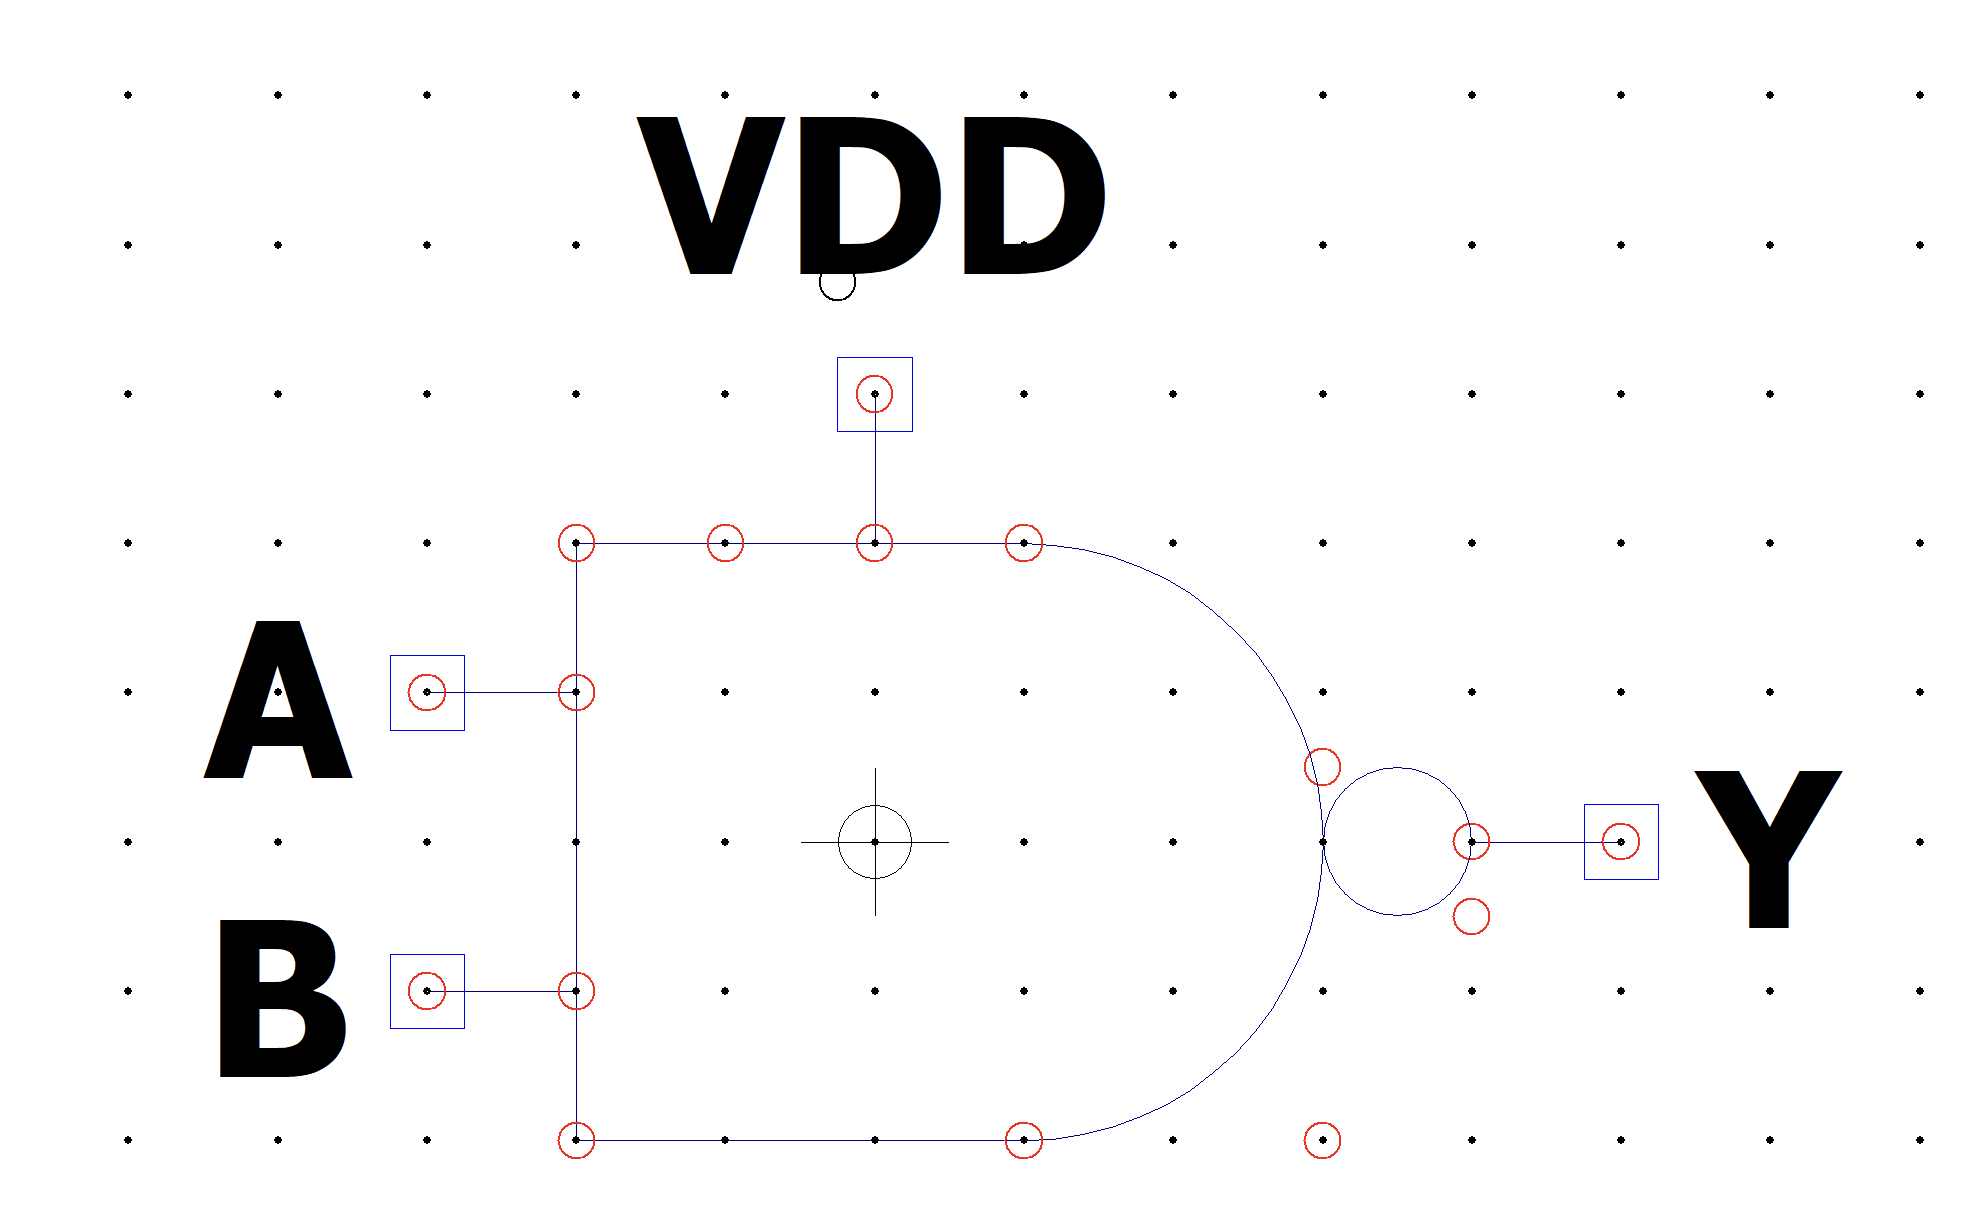
\includegraphics[scale=0.2]{image/symbol.png}
    \caption{Символ вентиля}
\end{figure}
\begin{figure}[H]
    \centering
    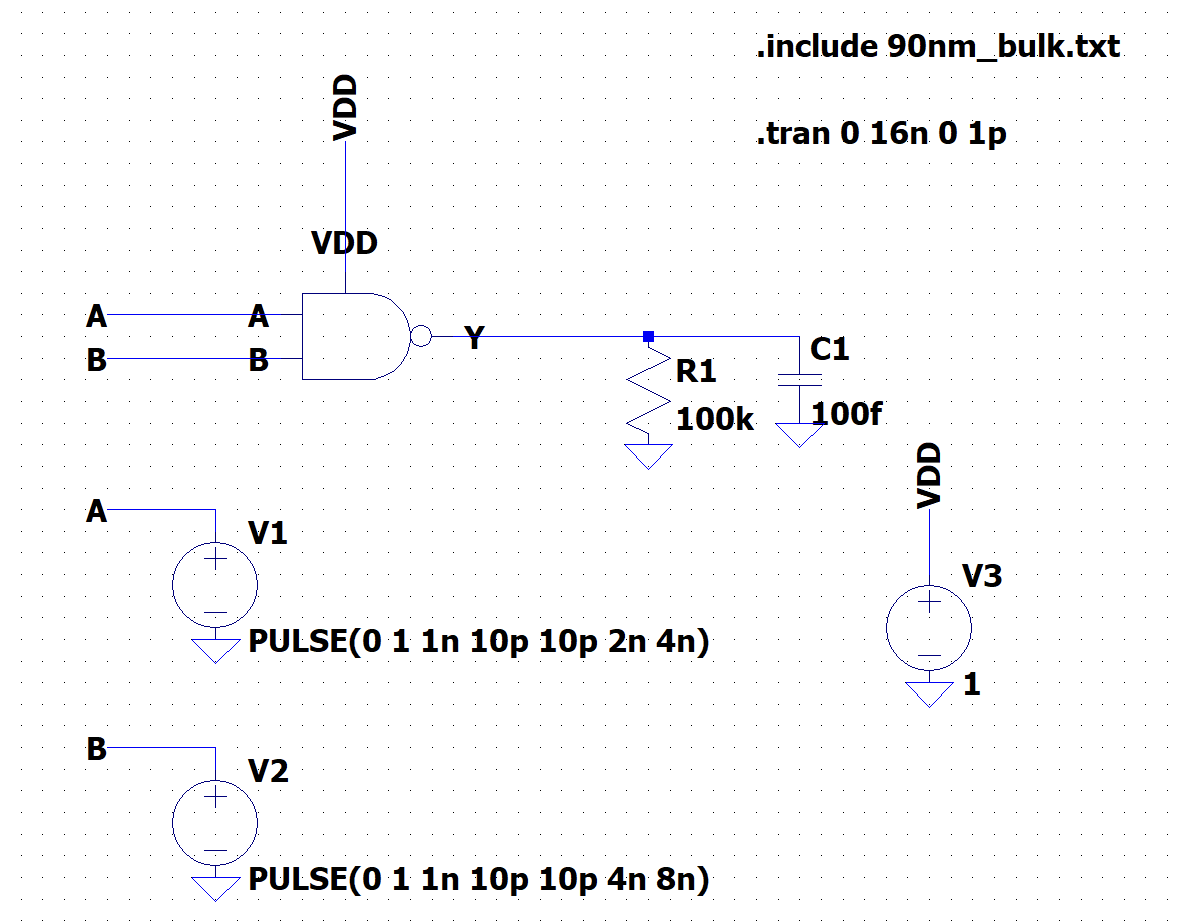
\includegraphics[width=\textwidth]{image/test-circuit.png}
    \caption{Схема тестирования}
\end{figure}
\subsection{Временная диаграмма процесса тестирования вентиля}
\begin{figure}[H]
    \centering
    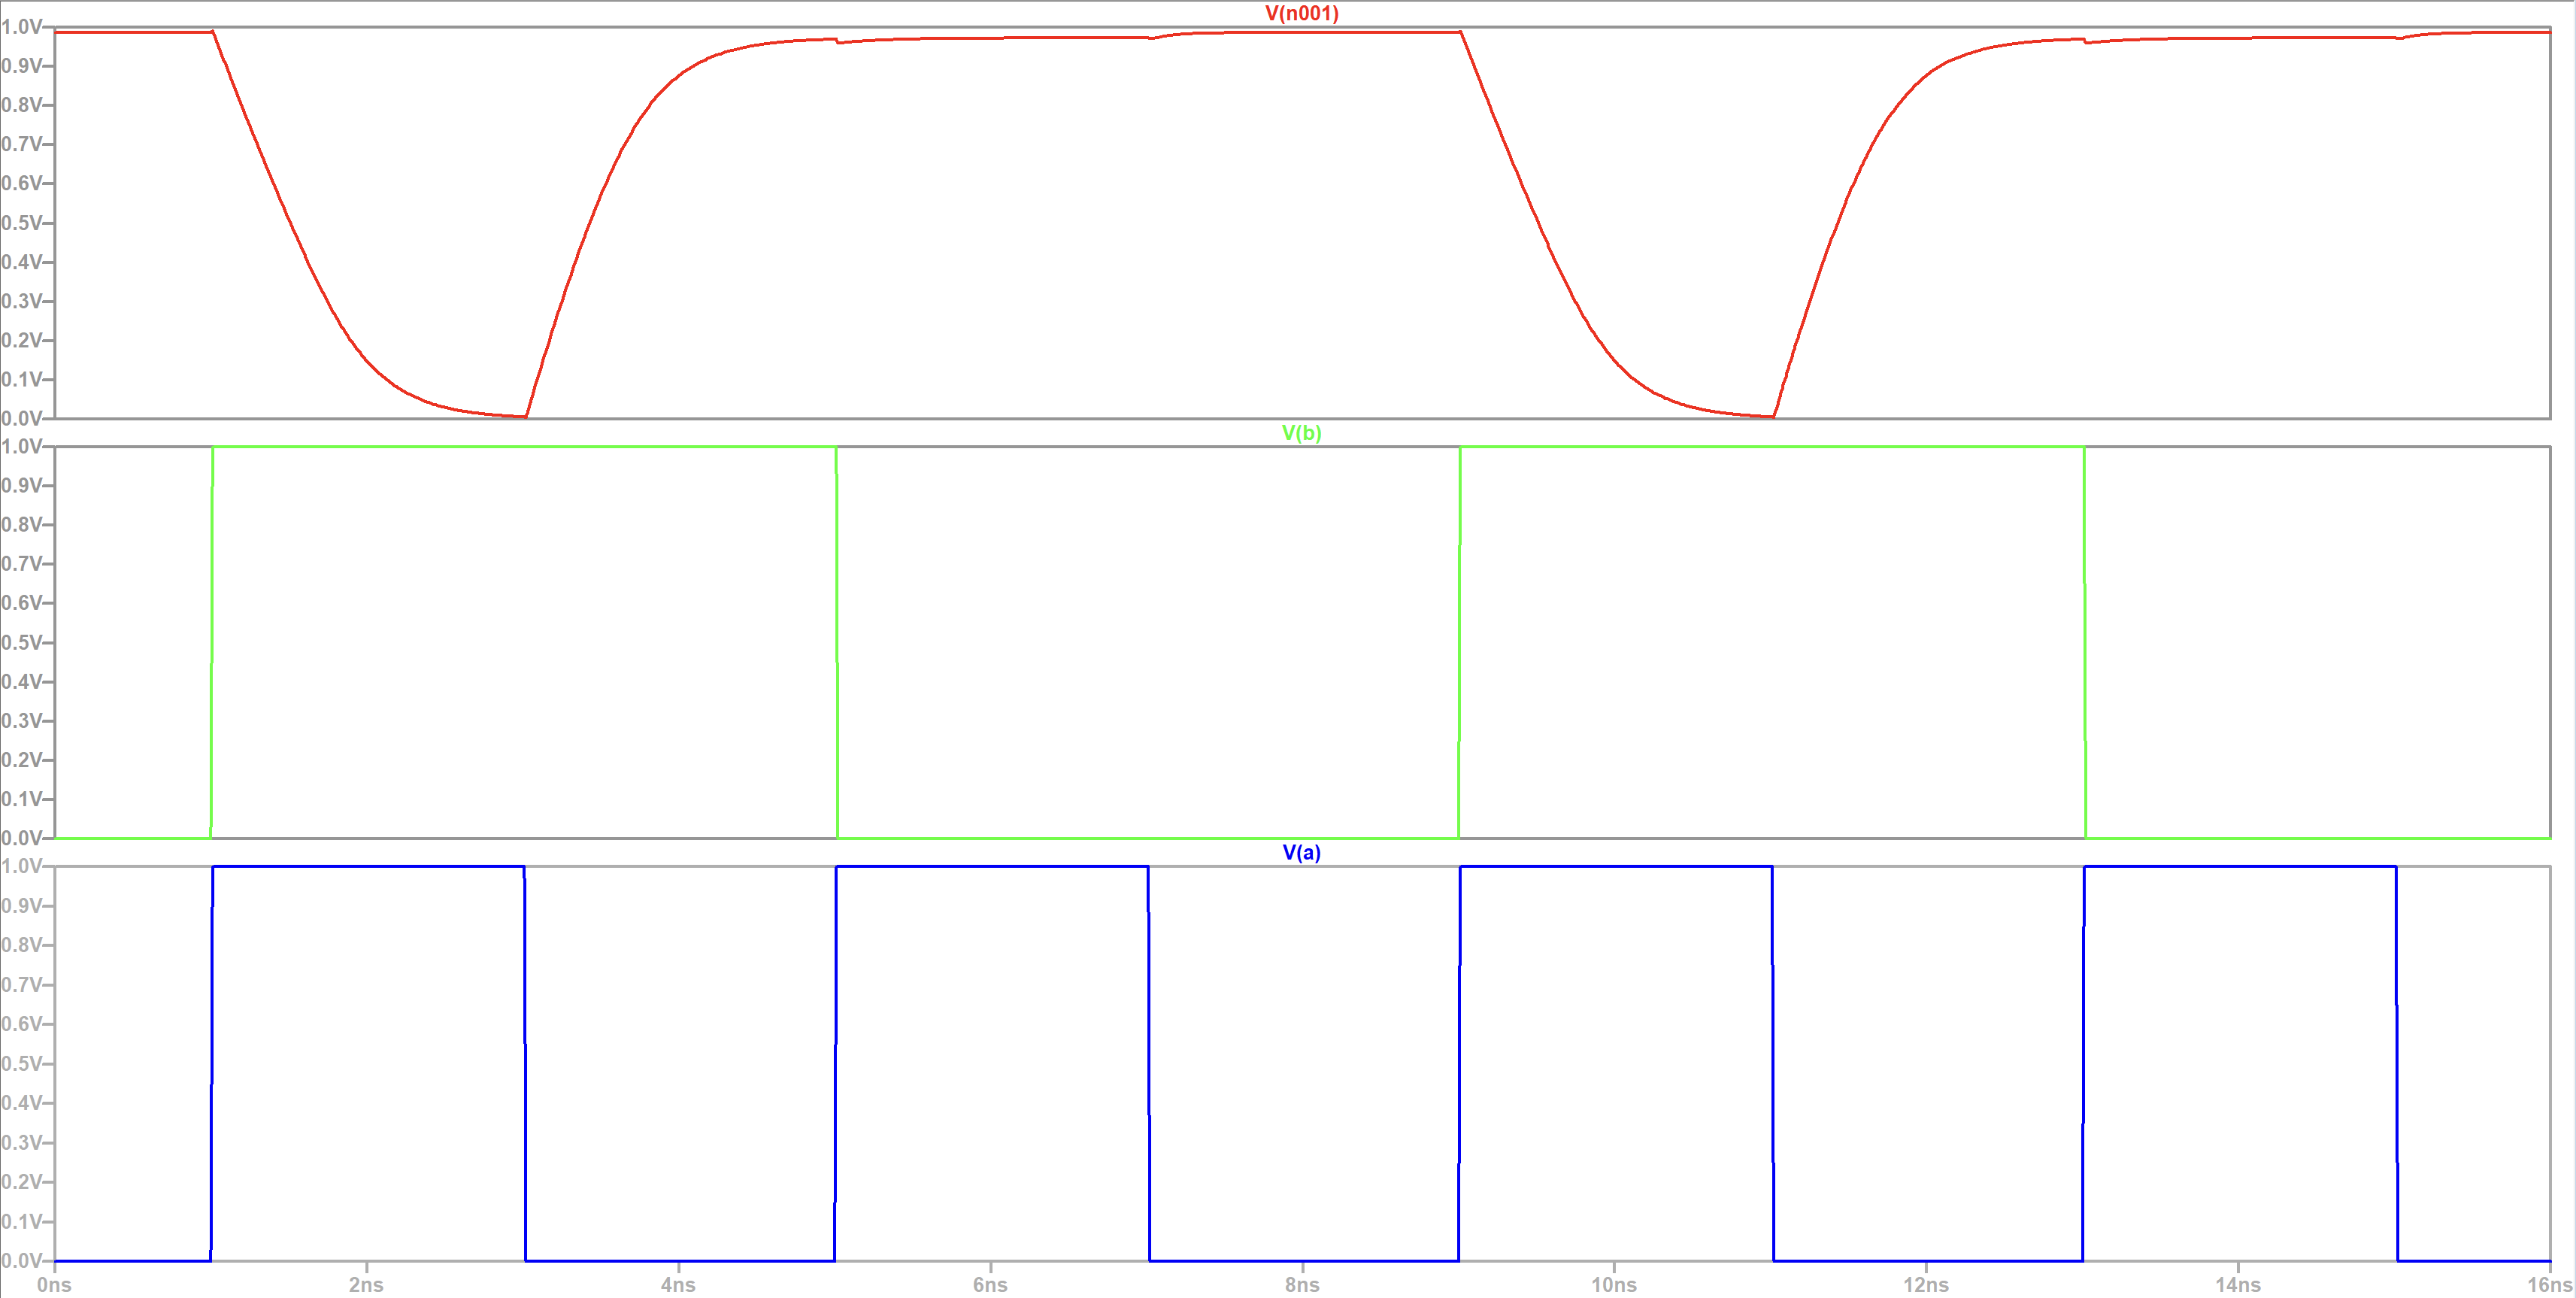
\includegraphics[width=\textwidth]{image/time-diagram.png}
    \caption{Временная диаграмма процесса тестирования вентиля}
\end{figure}
\subsection{Результат измерения задержки распространения сигнала через вентиль}
Задержка распространения - максимальное время от начала изменения входа до момента,
когда все выходы достигнут установившихся значений. Измеряется она между точками
перехода входным и выходным сигналом уровня 50\%.
\begin{figure}[H]
    \centering
    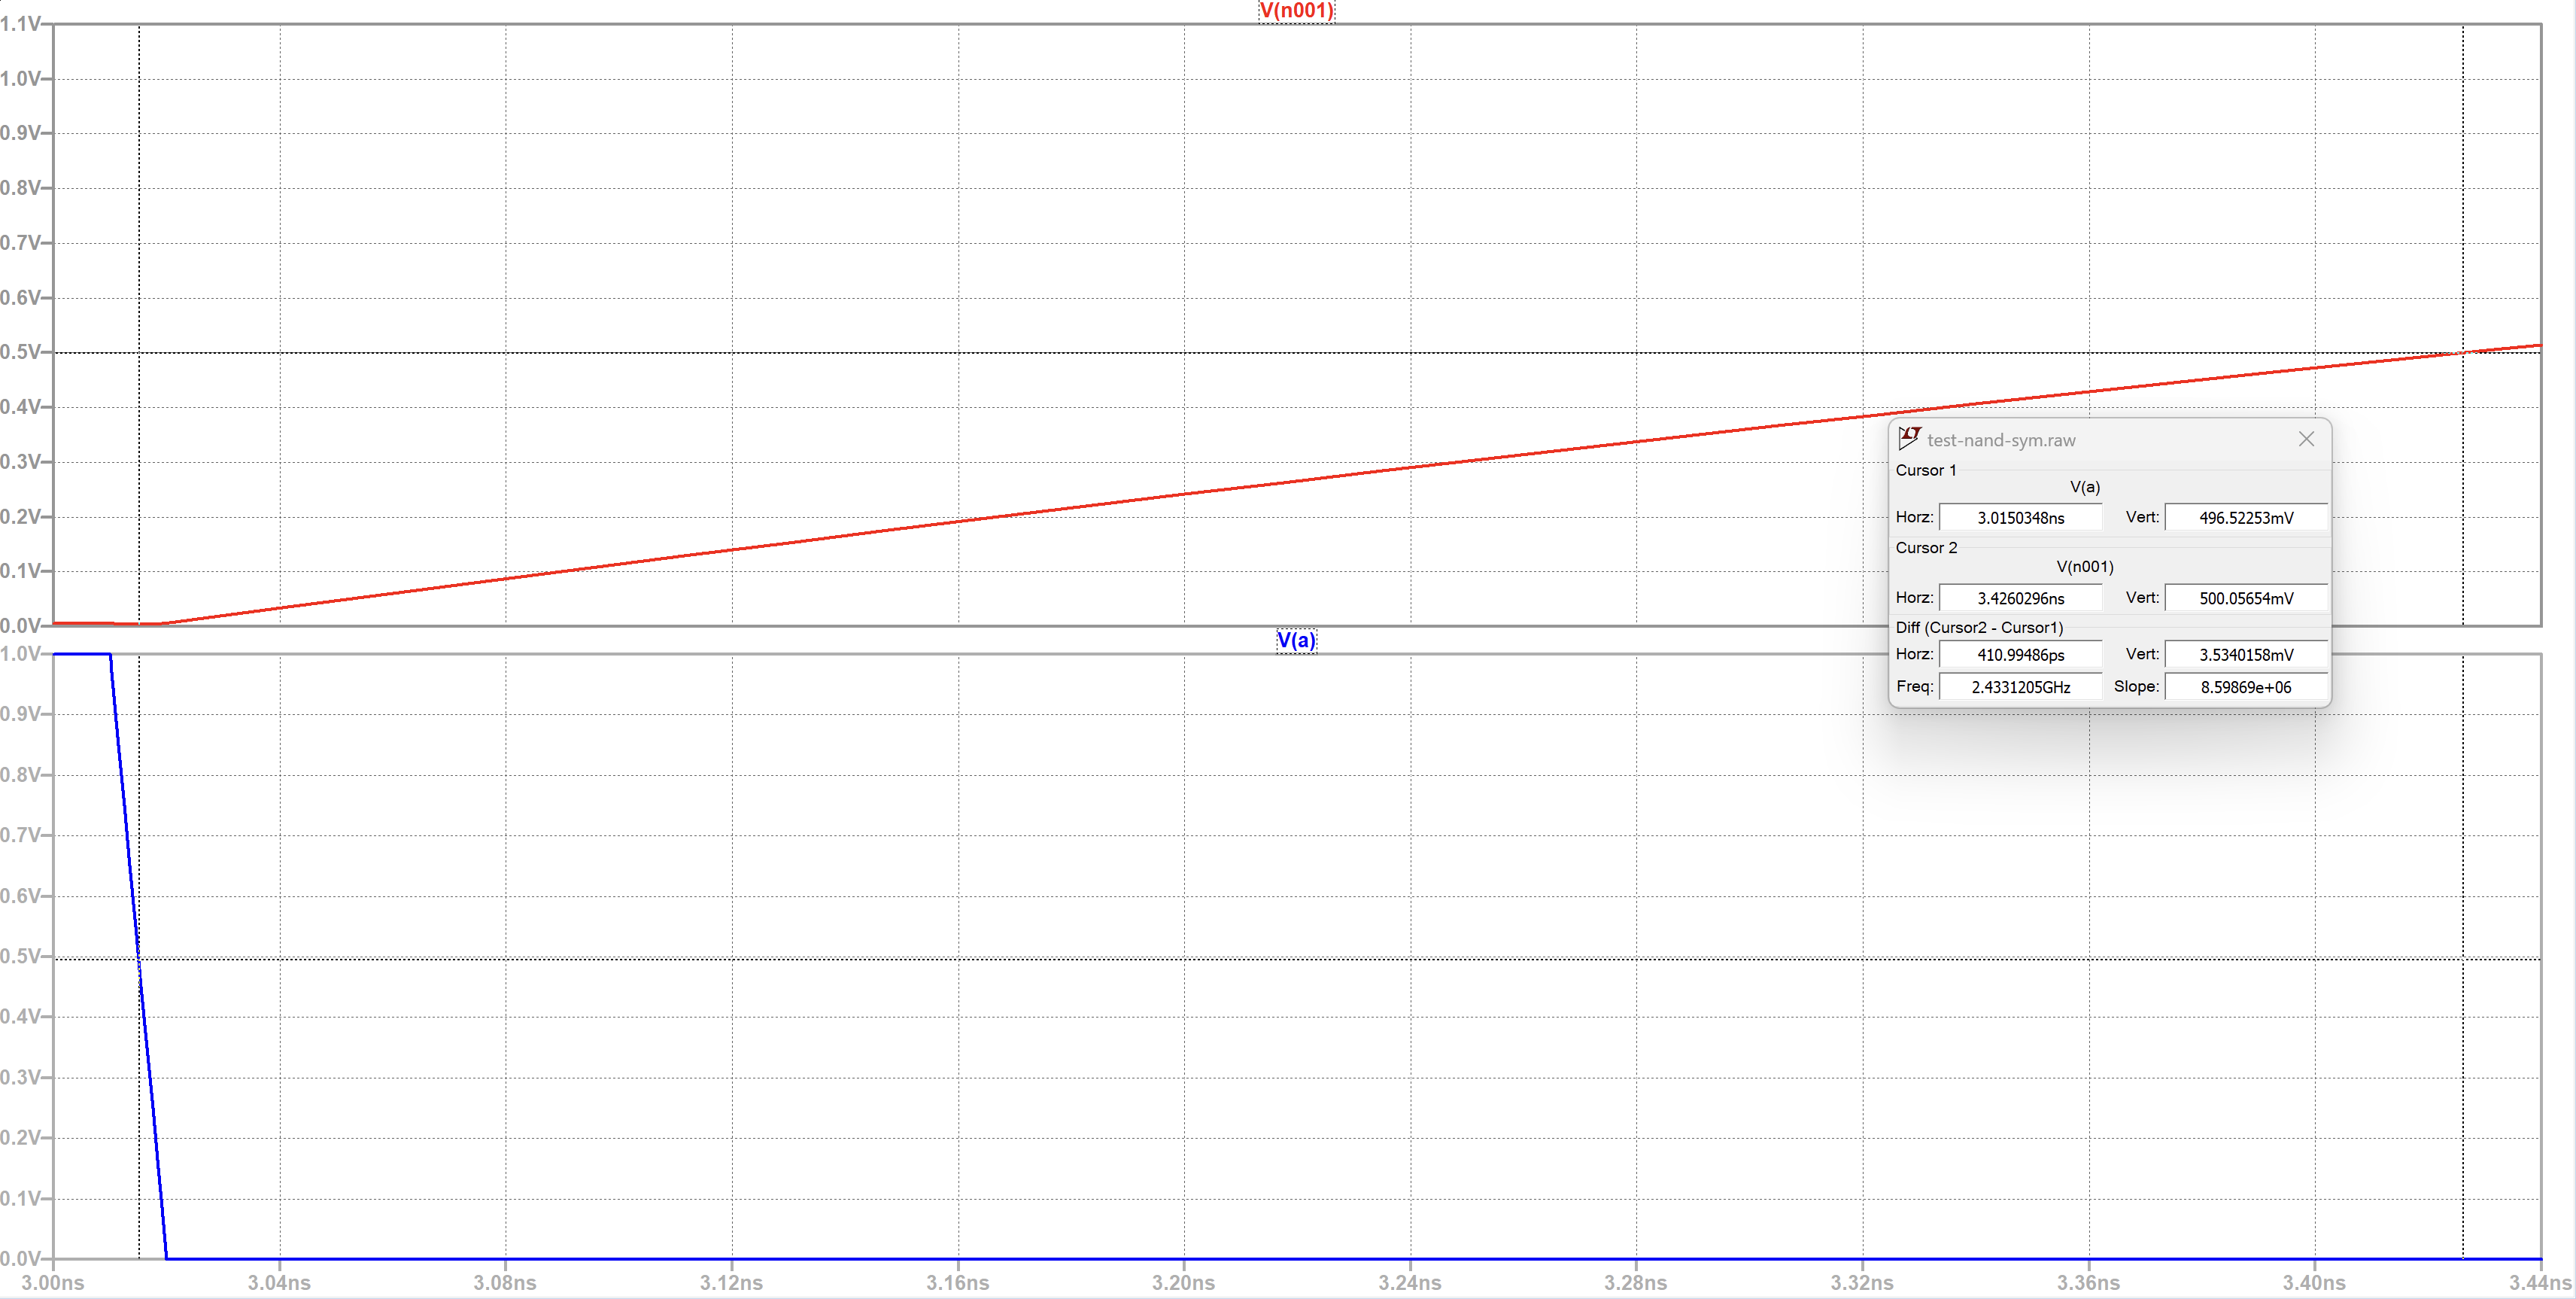
\includegraphics[width=\textwidth]{image/delay0-1.png}
    \caption{Подсчет задержки распространения сигнала для 0-1 на выходе}
\end{figure}
\begin{figure}[H]
    \centering
    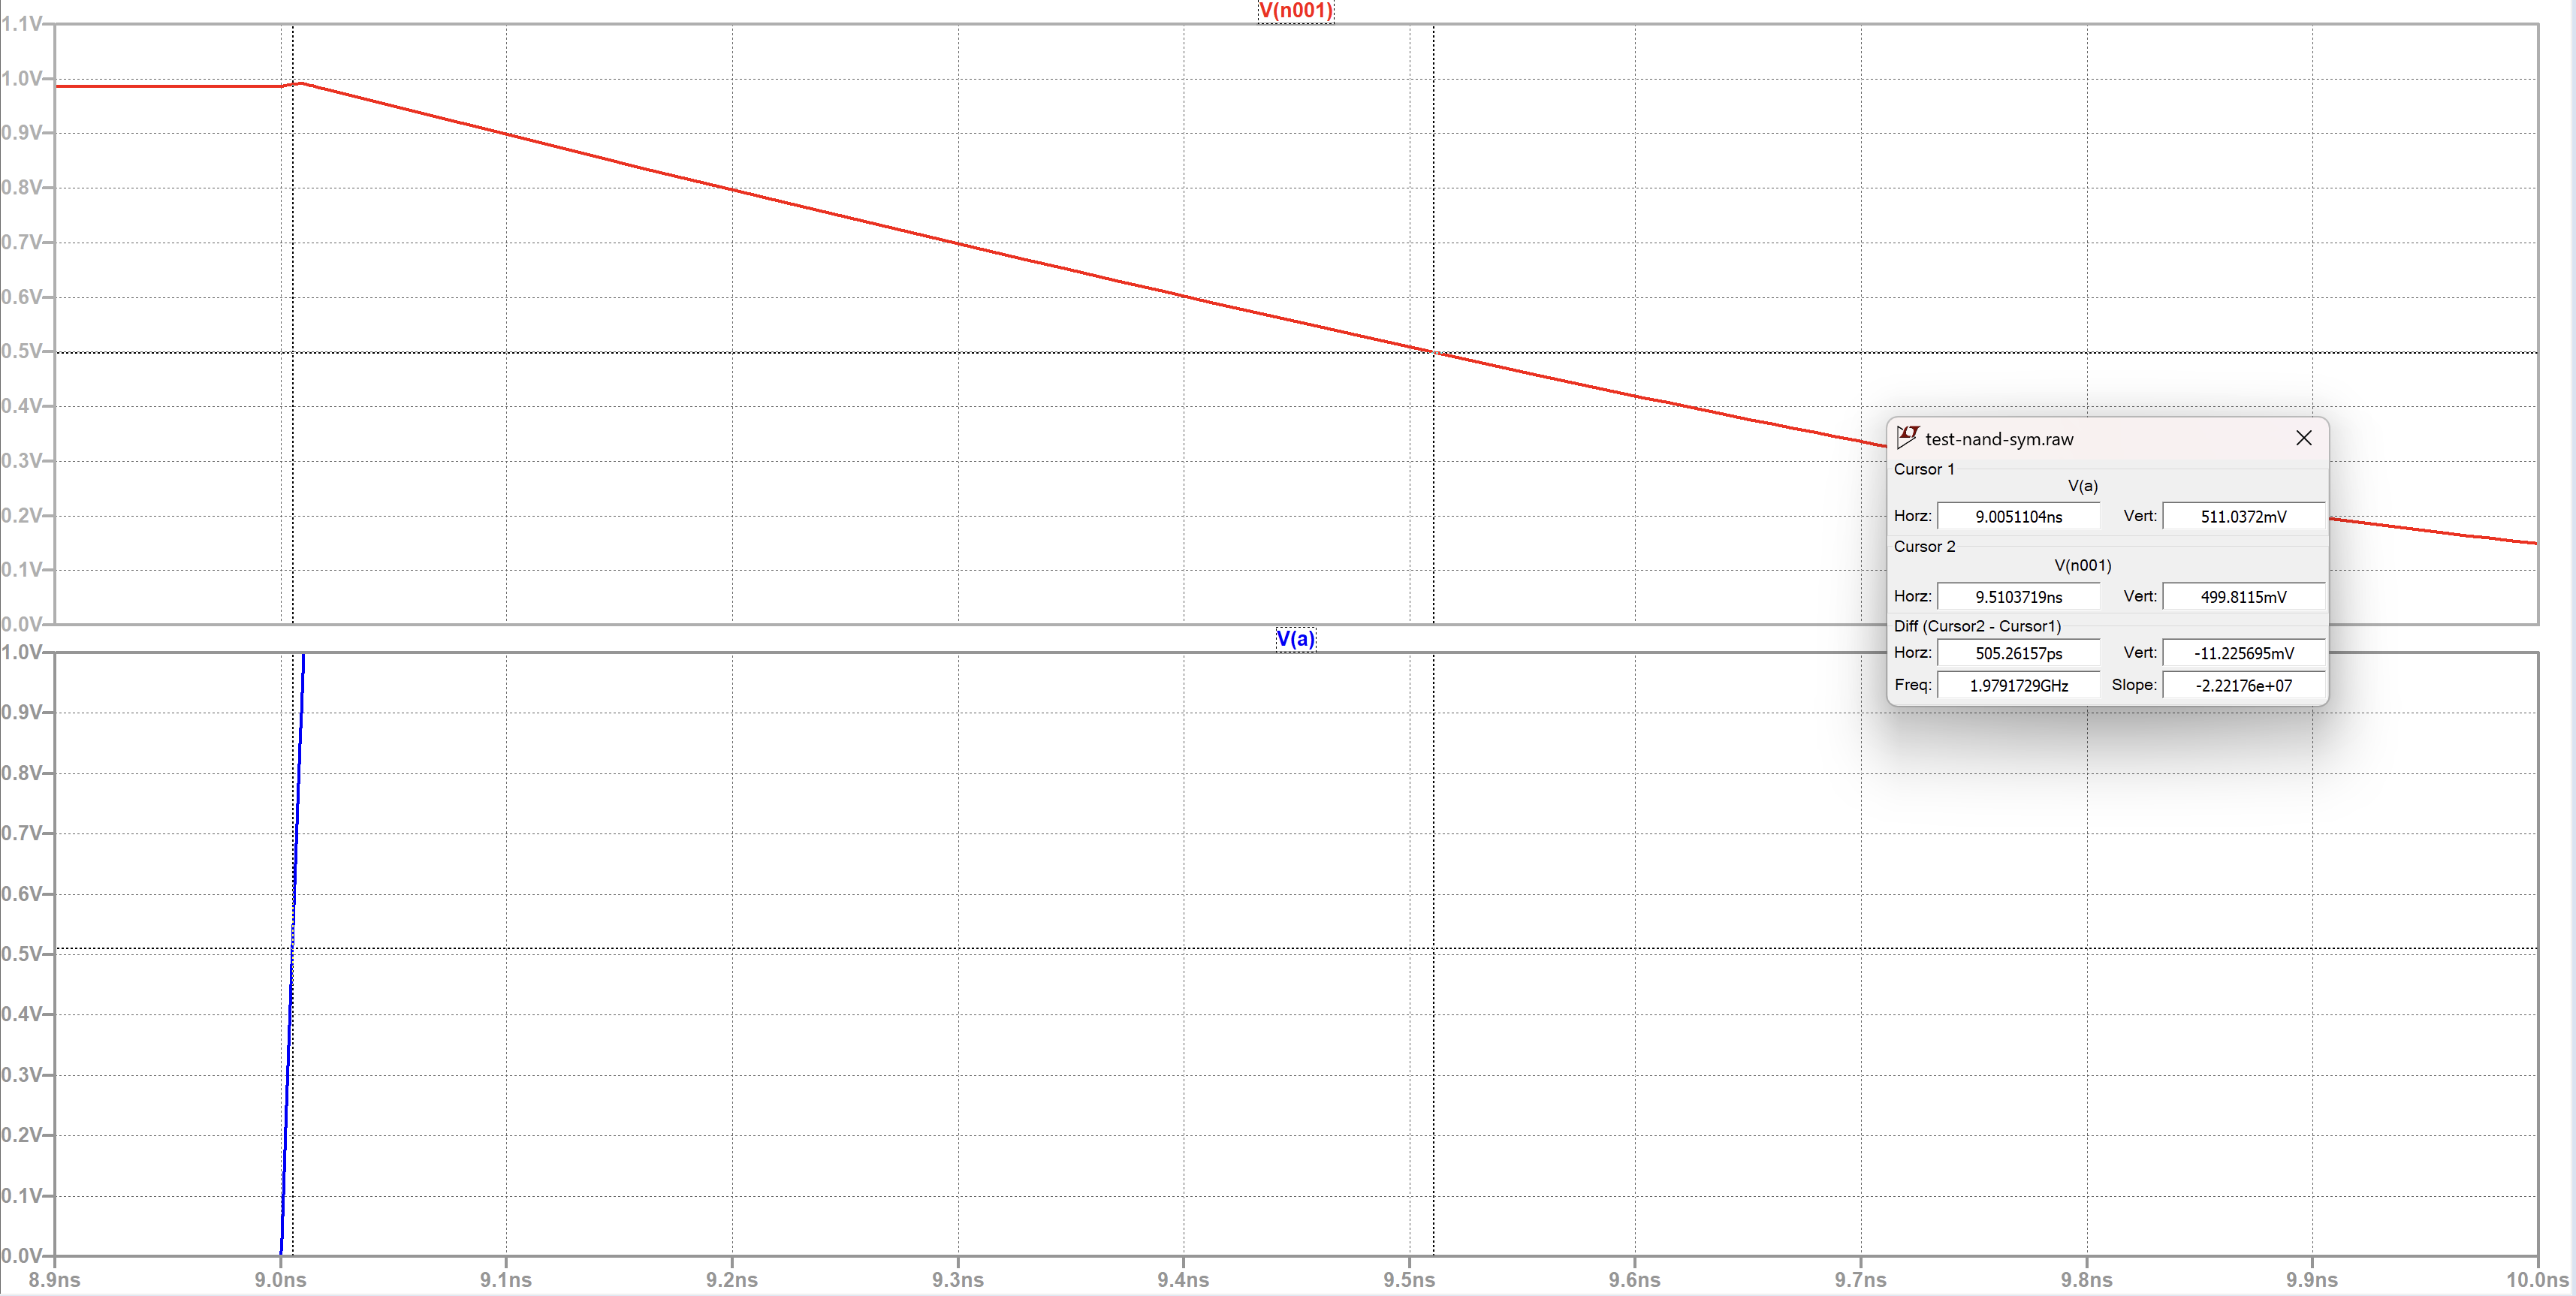
\includegraphics[width=\textwidth]{image/delay1-0.png}
    \caption{Подсчет задержки распространения сигнала для 1-0 на выходе}
\end{figure}
$$
    t_{pd} = t_2 - t_1 = 3.426 - 3.015 = 0.411 \text{нс} - \text{задержка распространения сигнала для 0-1 на выходе}
$$
$$
    t_{pd} = t_2 - t_1 = 9.510 - 9.005 = 0.505 \text{нс} - \text{задержка распространения сигнала для 1-0 на выходе}
$$
\subsection{Максимальная частота работы вентиля}
Высчитывается как время спада(фронта) от 0.1 до 0.9 (0.9 до 0.1) уровня на выходе вентиля, и от этого времени высчитывается частота:
\begin{figure}
    \centering
    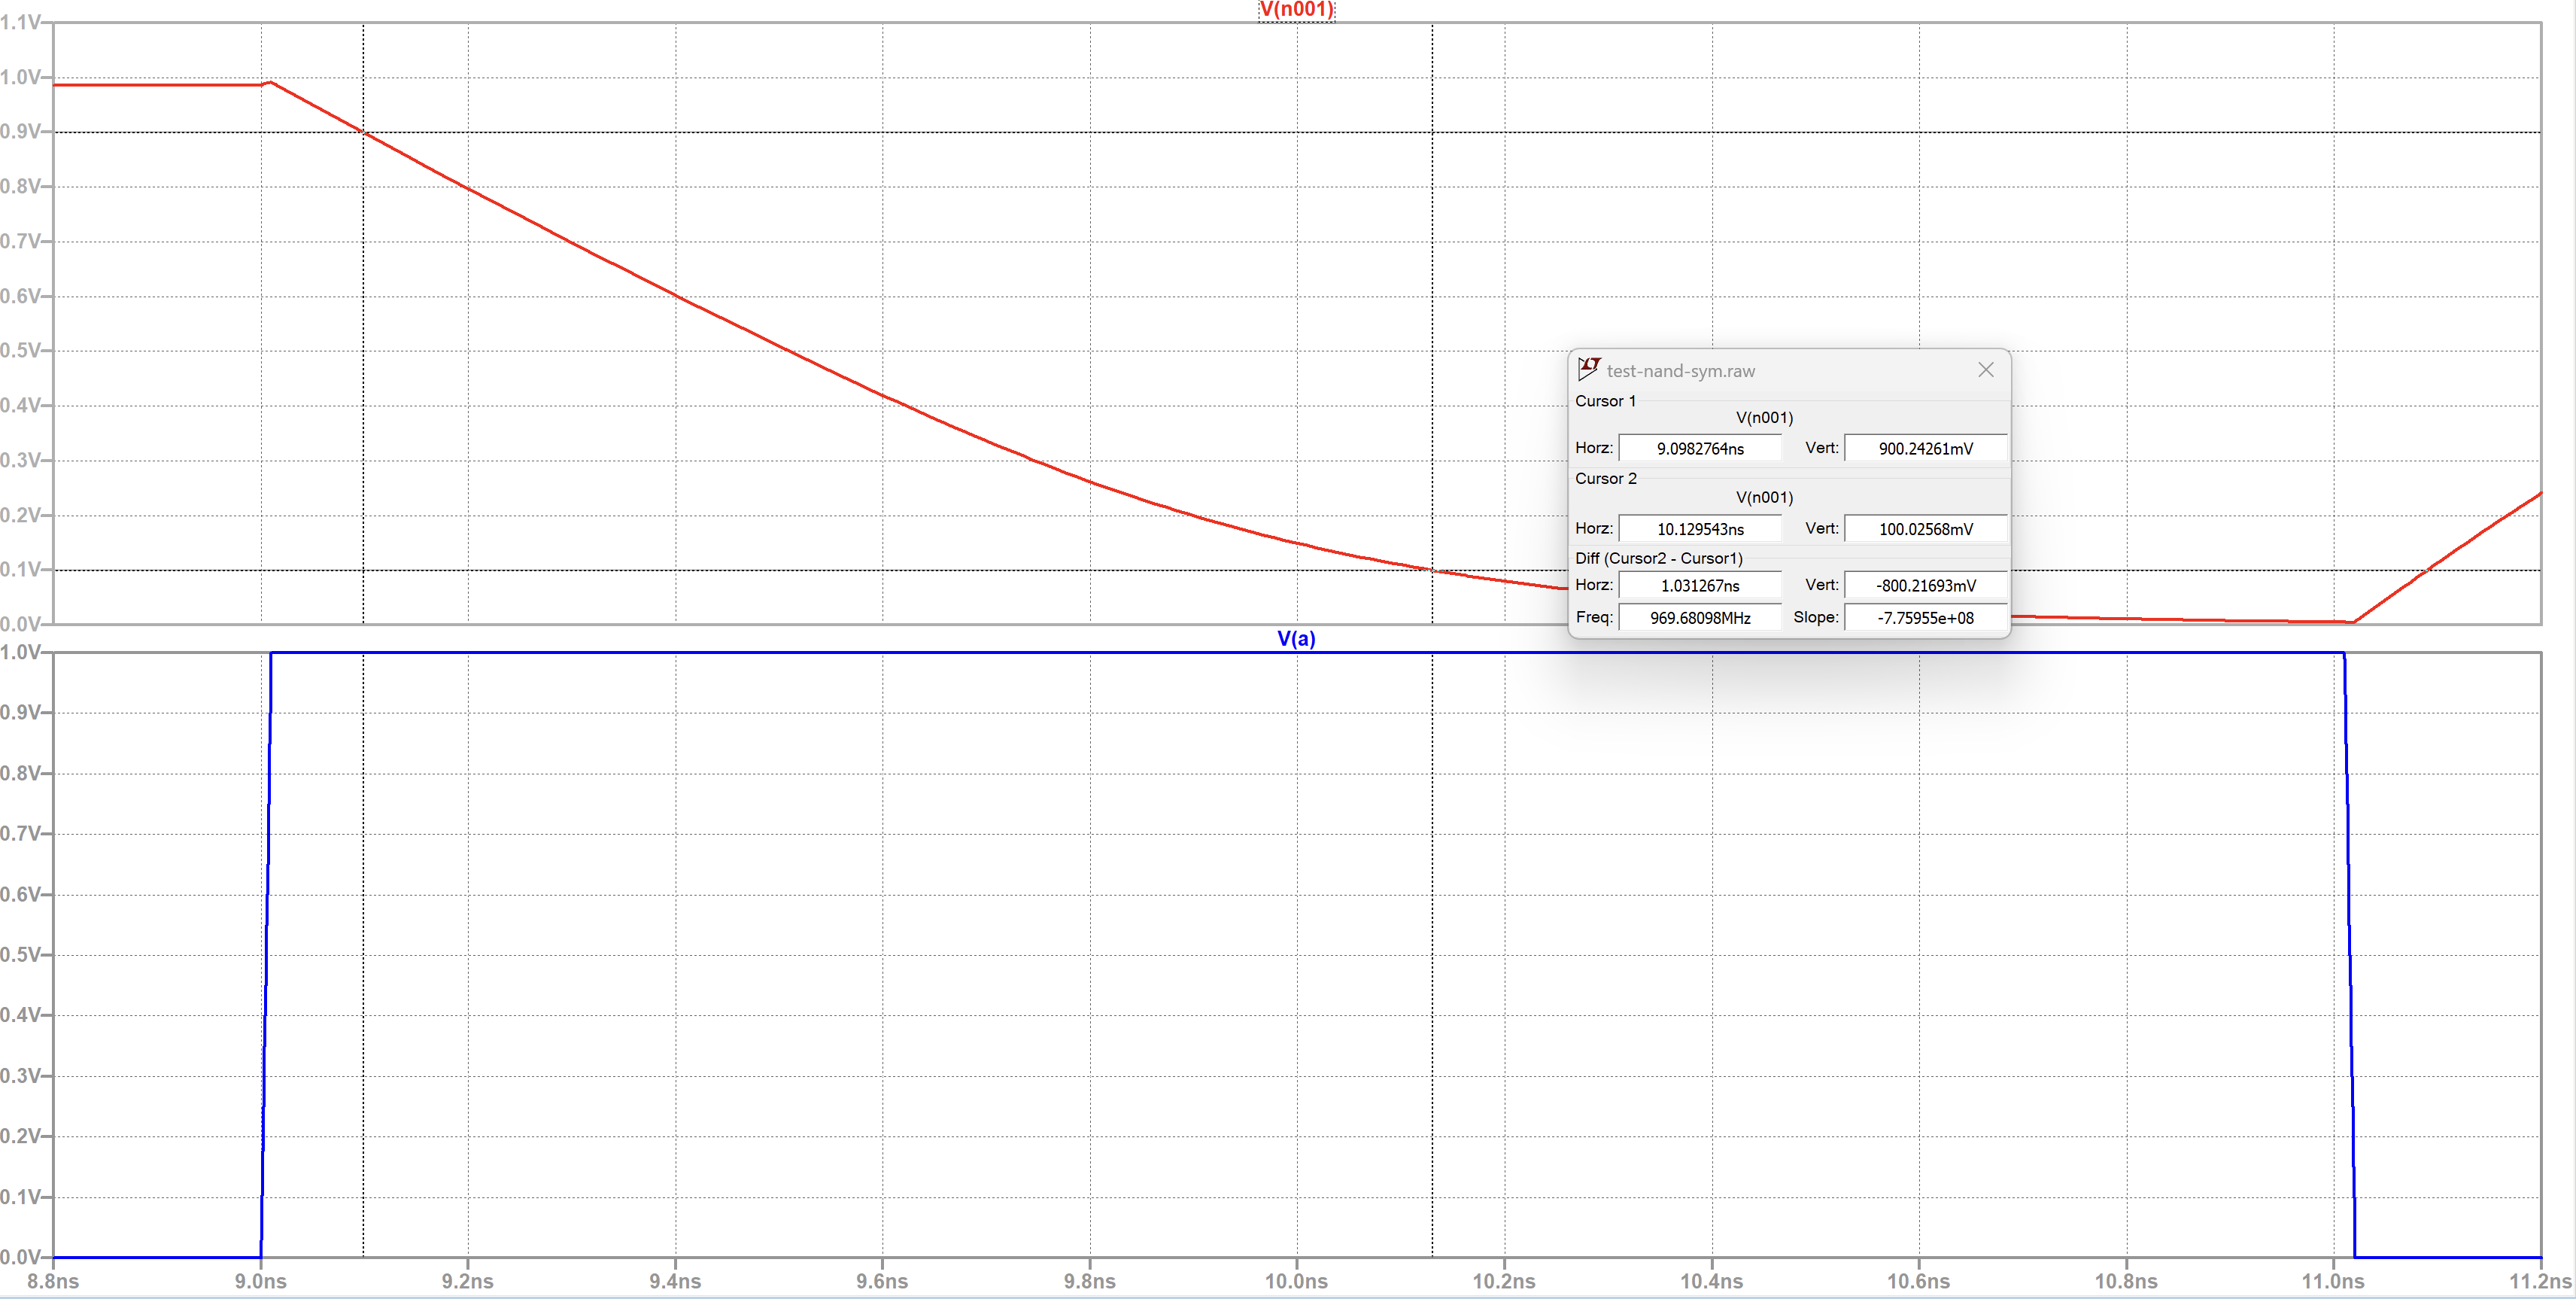
\includegraphics[width=\textwidth]{image/frequency10.png}
    \caption{Время спада от 0.9 до 0.1}
\end{figure}
\begin{figure}[H]
    \centering
    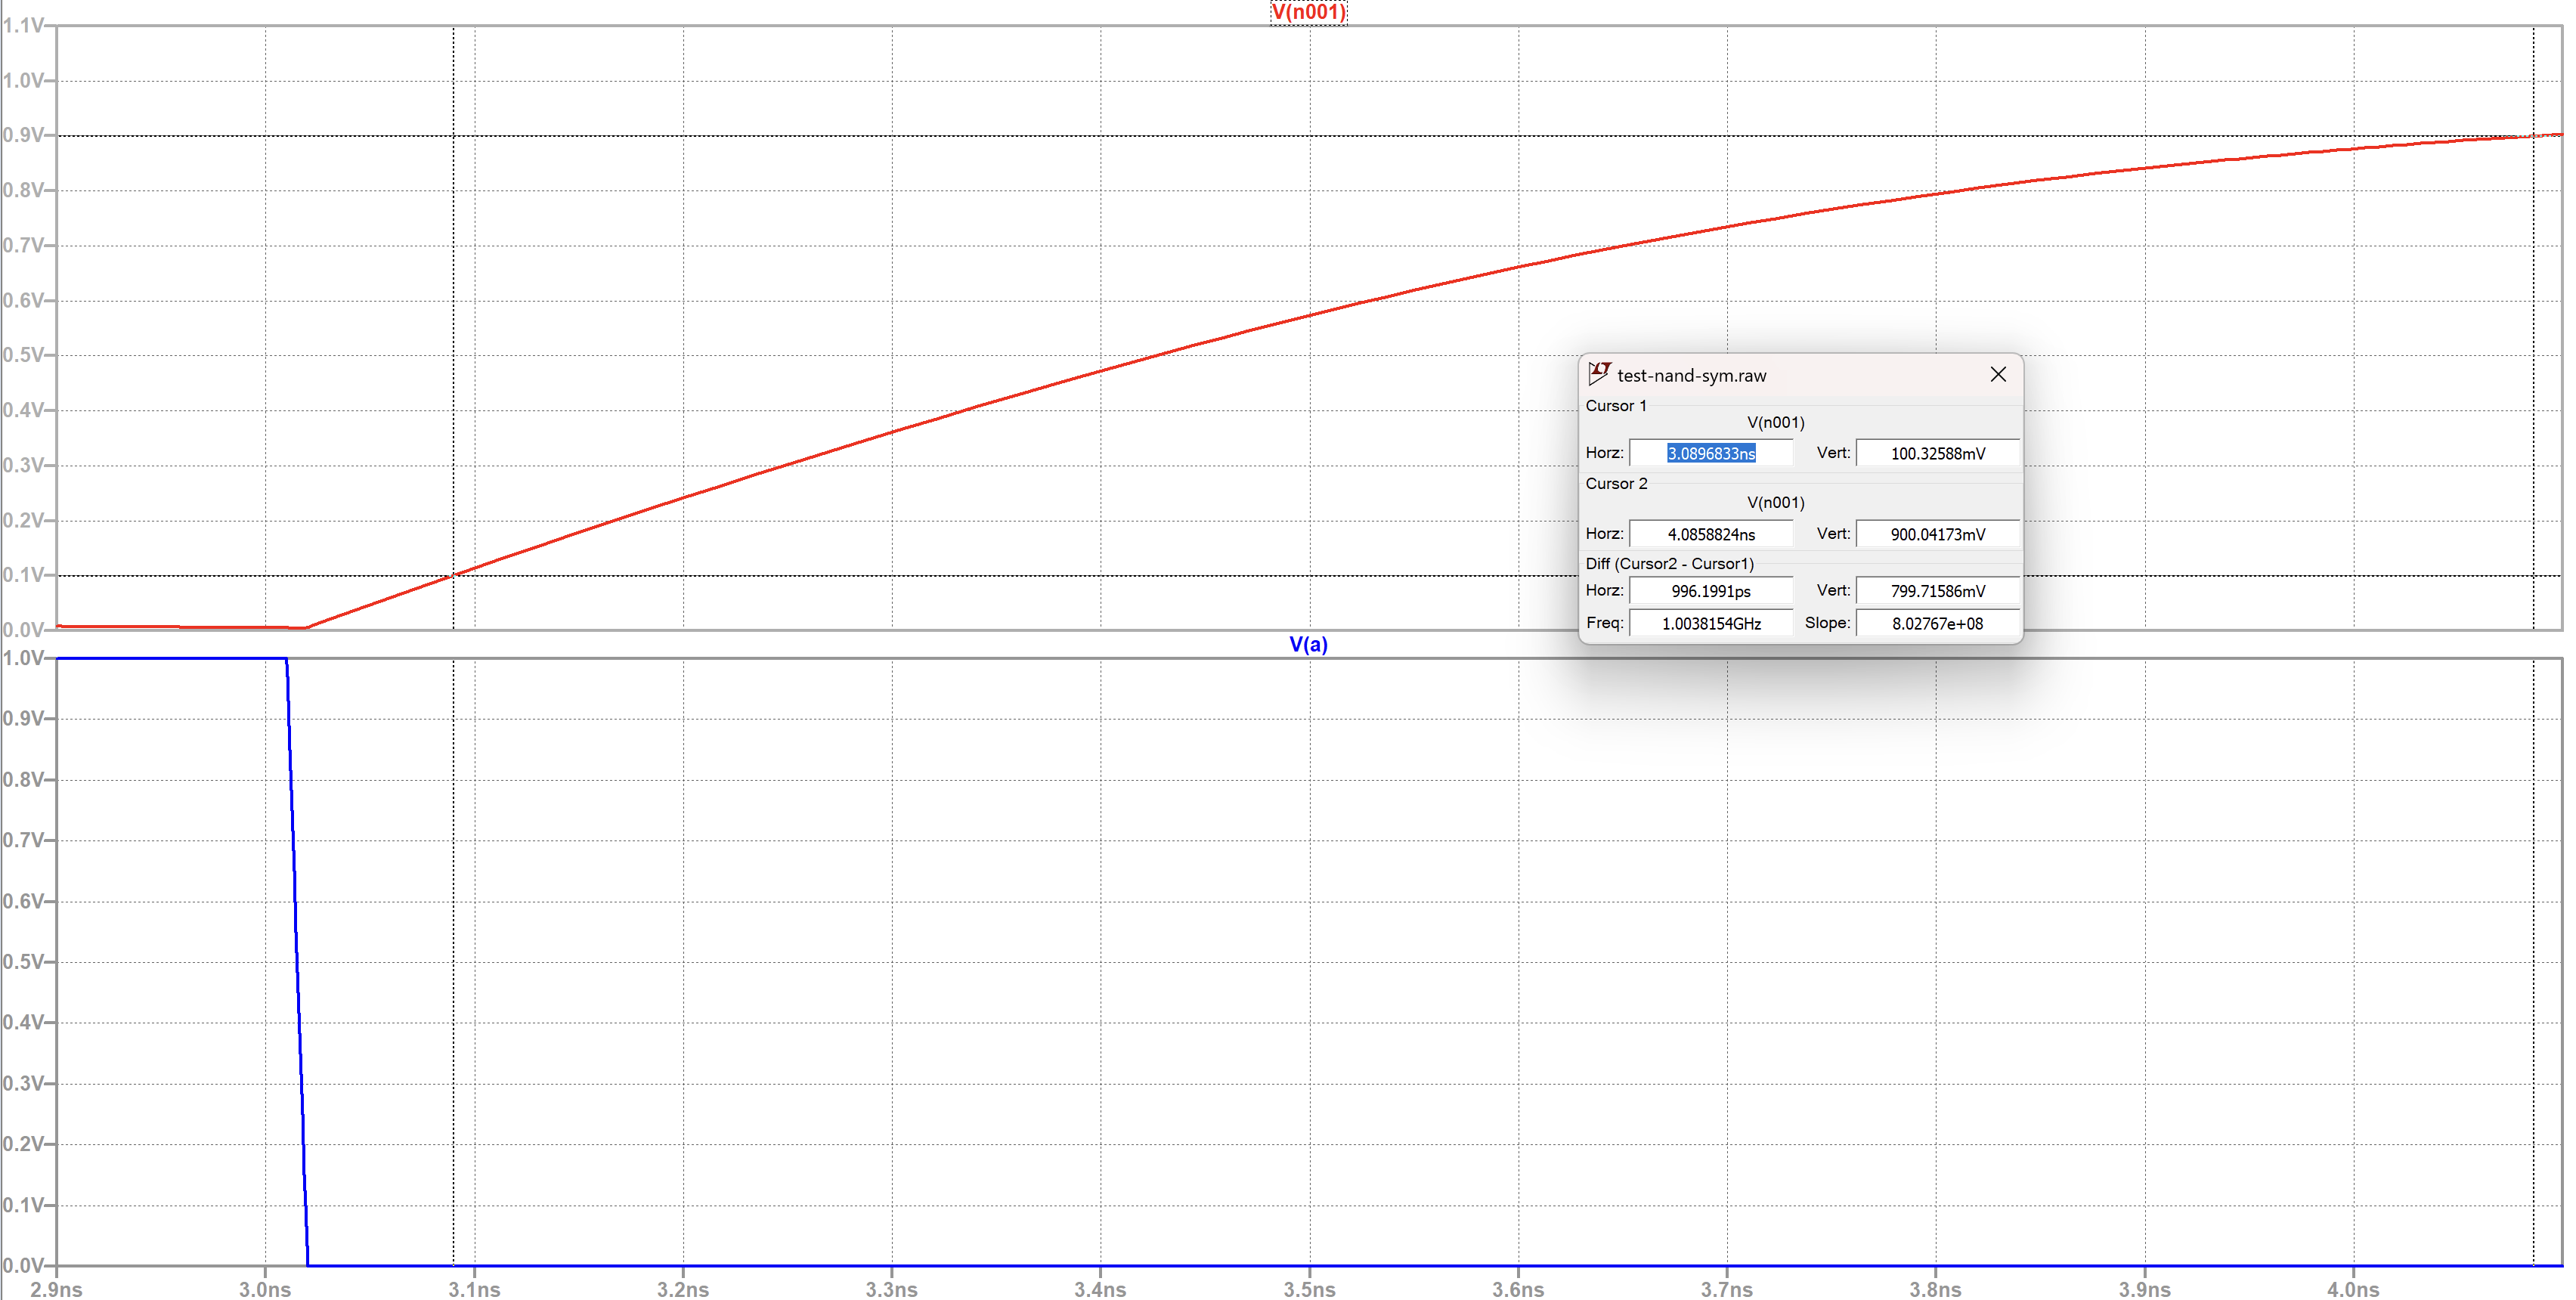
\includegraphics[width=\textwidth]{image/frequency01.png}
    \caption{Время фронта от 0.1 до 0.9}
\end{figure}
$$
    t_{10} = 9.098 - 10.130 = 1.031 \text{нс} - \text{для спада}
$$
$$t_{01} = 4.086 - 3.089 = 0.996 \text{нс} - \text{для фронта}$$
Тогда частота спада/фронта:
$$
    \nu_{\text{спада}} = \frac{1}{t_{10}} = \frac{1}{1.031} = 0.970 \text{ГГц}
$$
$$
    \nu_{\text{фронта}} = \frac{1}{t_{01}} = \frac{1}{0.996} = 1.004 \text{ГГц}
$$
Тогда максимальная частота работы вентиля:
$$
\nu_{\max} = \min(\nu_{\text{спада}}, \nu_{\text{фронта}}) = \min(0.970, 1.004) = 0.970 \text{ГГц}
$$
\subsection{Постройте БОЭ на базе созданного вентиля согласно варианту задания.}
Полный четырех разрядный компаратор.
$$
\begin{aligned}
    & (A = B)- \overline{\bar{A} B \vee A \bar{B}}=\overline{\overline{\overline{\bar{A} B} \wedge \overline{\bar{A} \bar{B}}}}
= \overline{\overline{(\bar{A} \mid B)(A \mid \bar{B})}}=\overline{(\bar{A} \mid B) \mid(A \mid \bar{B})}\\
& (A<B)-\bar{A} B=\overline{\overline{\bar{A} B}}=\overline{(\bar{A} \mid B)} \\
& (A>B)-A \bar{B}=\overline{\overline{A B}}=(\overline{A \mid \bar{B}})\\
& \bar{A} = (A \mid A)
\end{aligned}
$$
\begin{figure}[H]
    \centering
    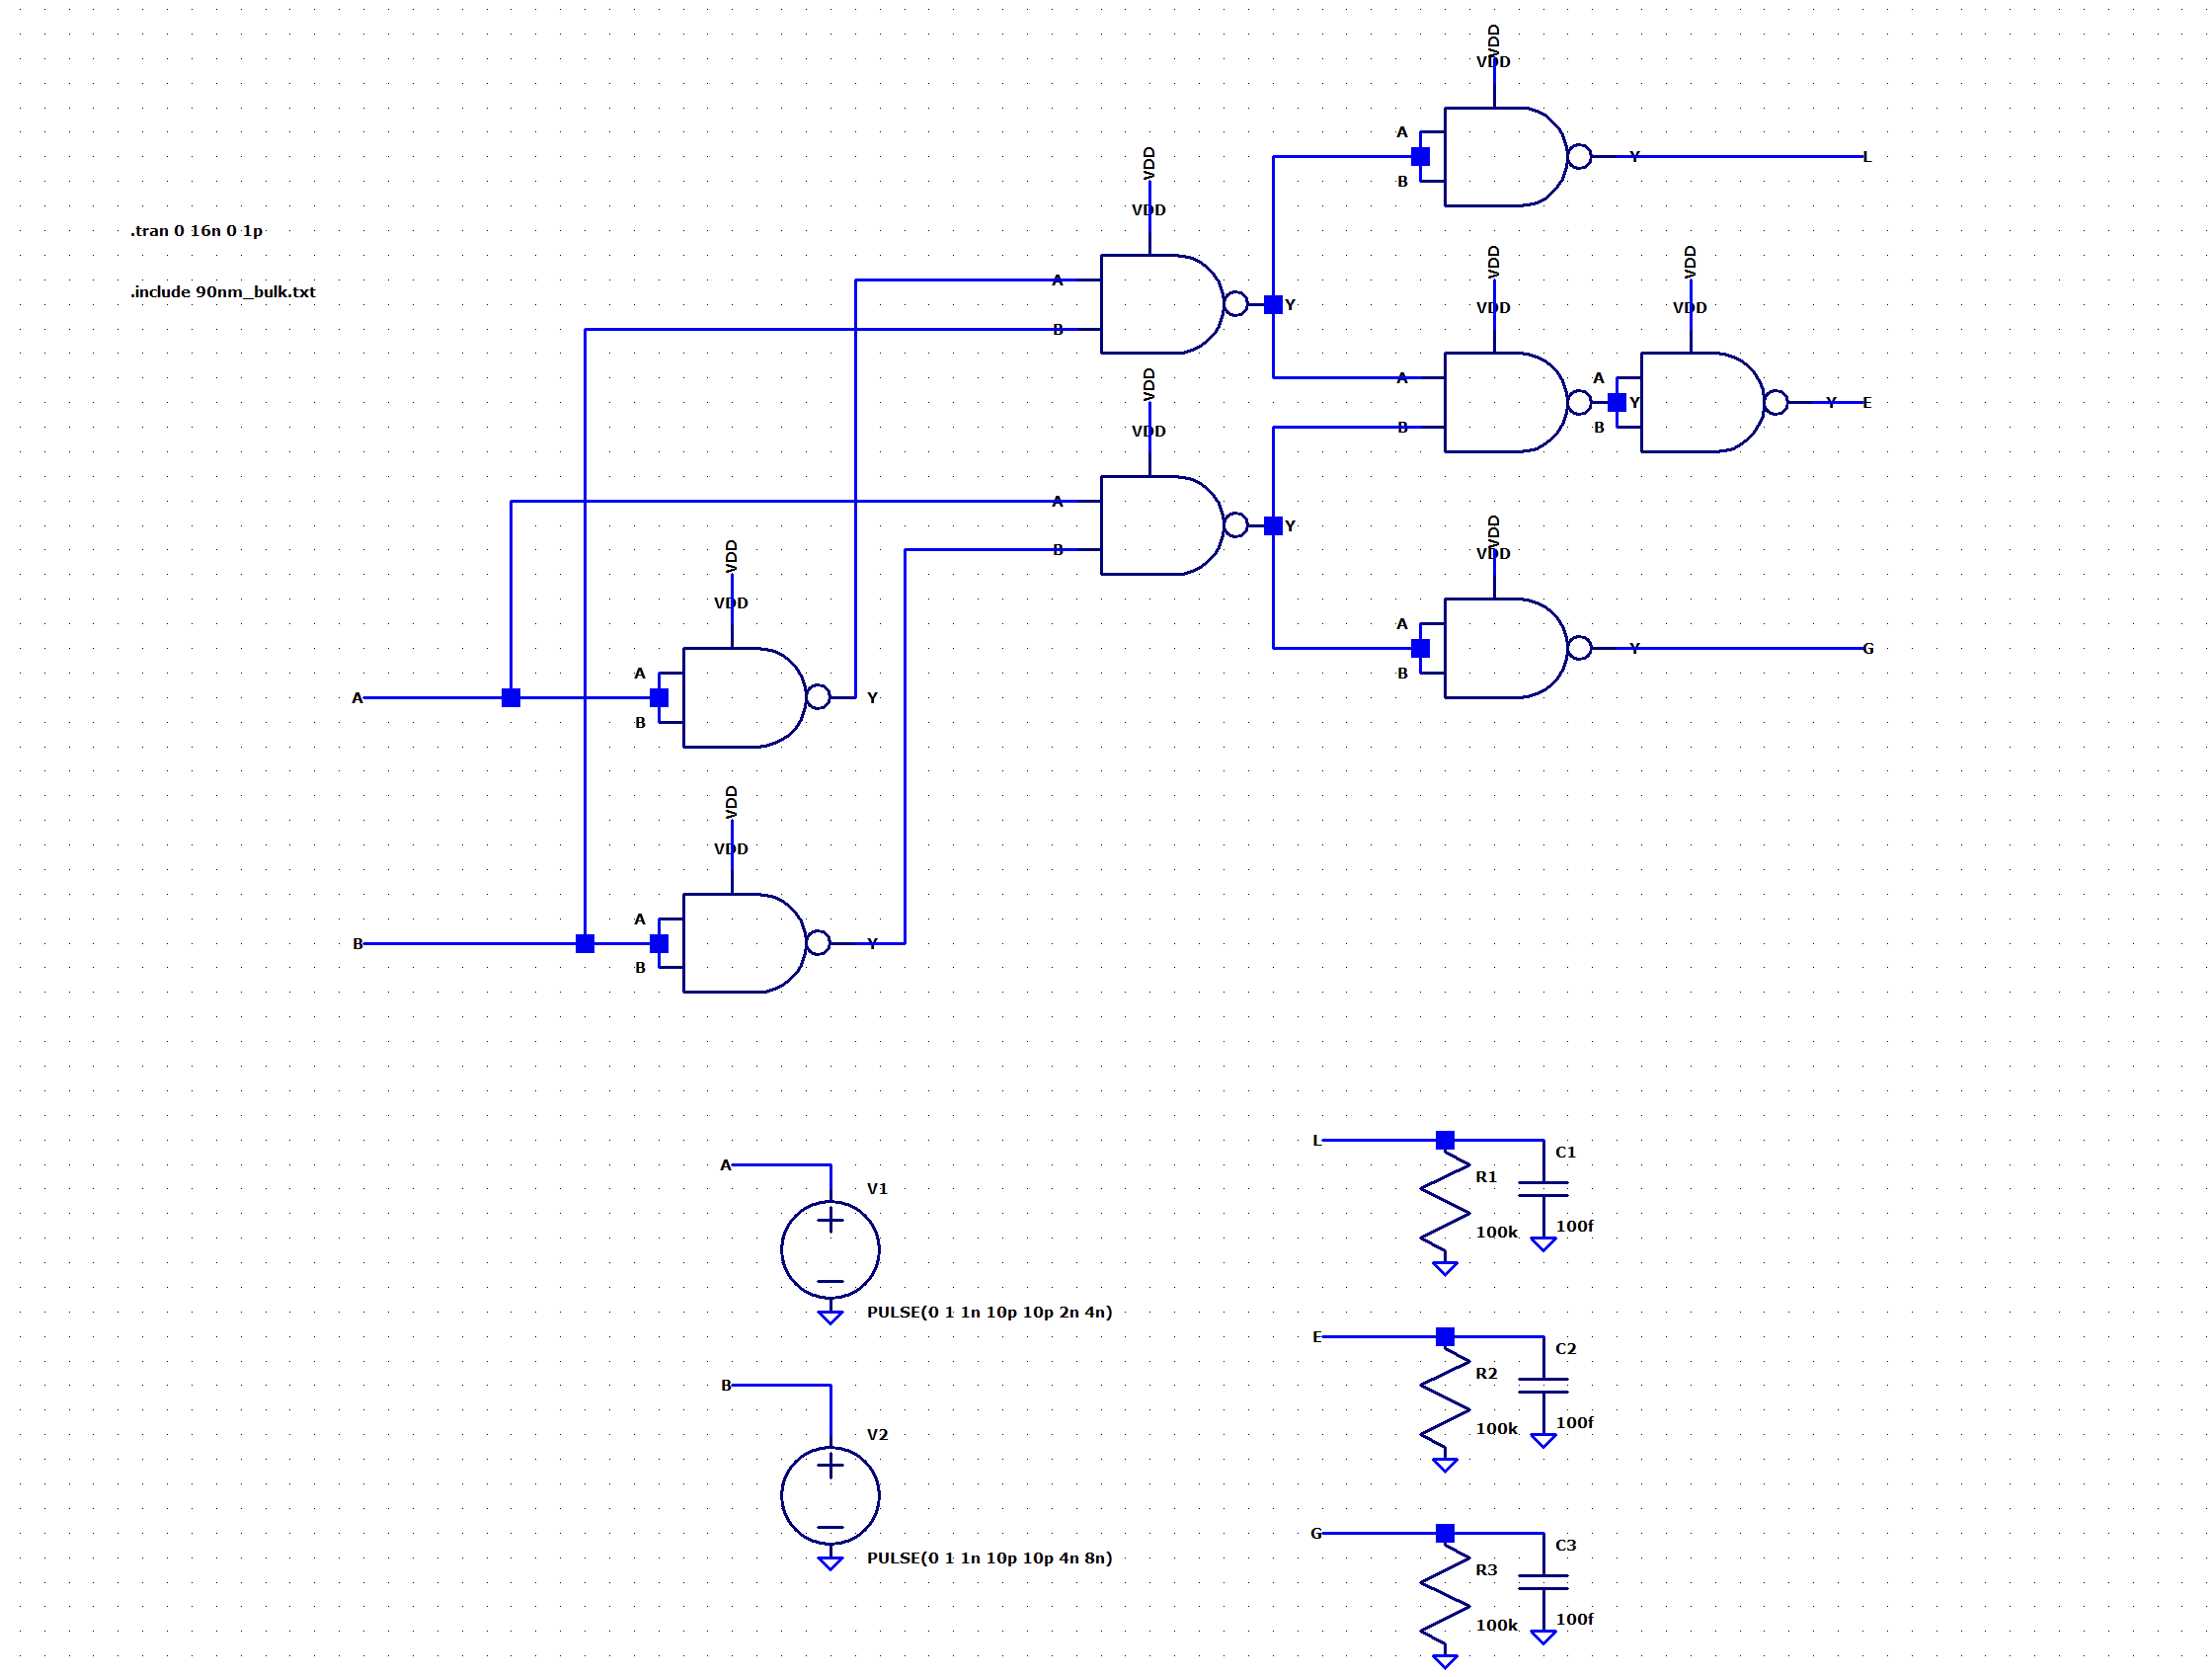
\includegraphics[width=\textwidth]{image/full-comparator1.png}
    \caption{Схема полного компаратора с двумя одноразрядными входами}
\end{figure}
\begin{figure}[H]
    \centering
    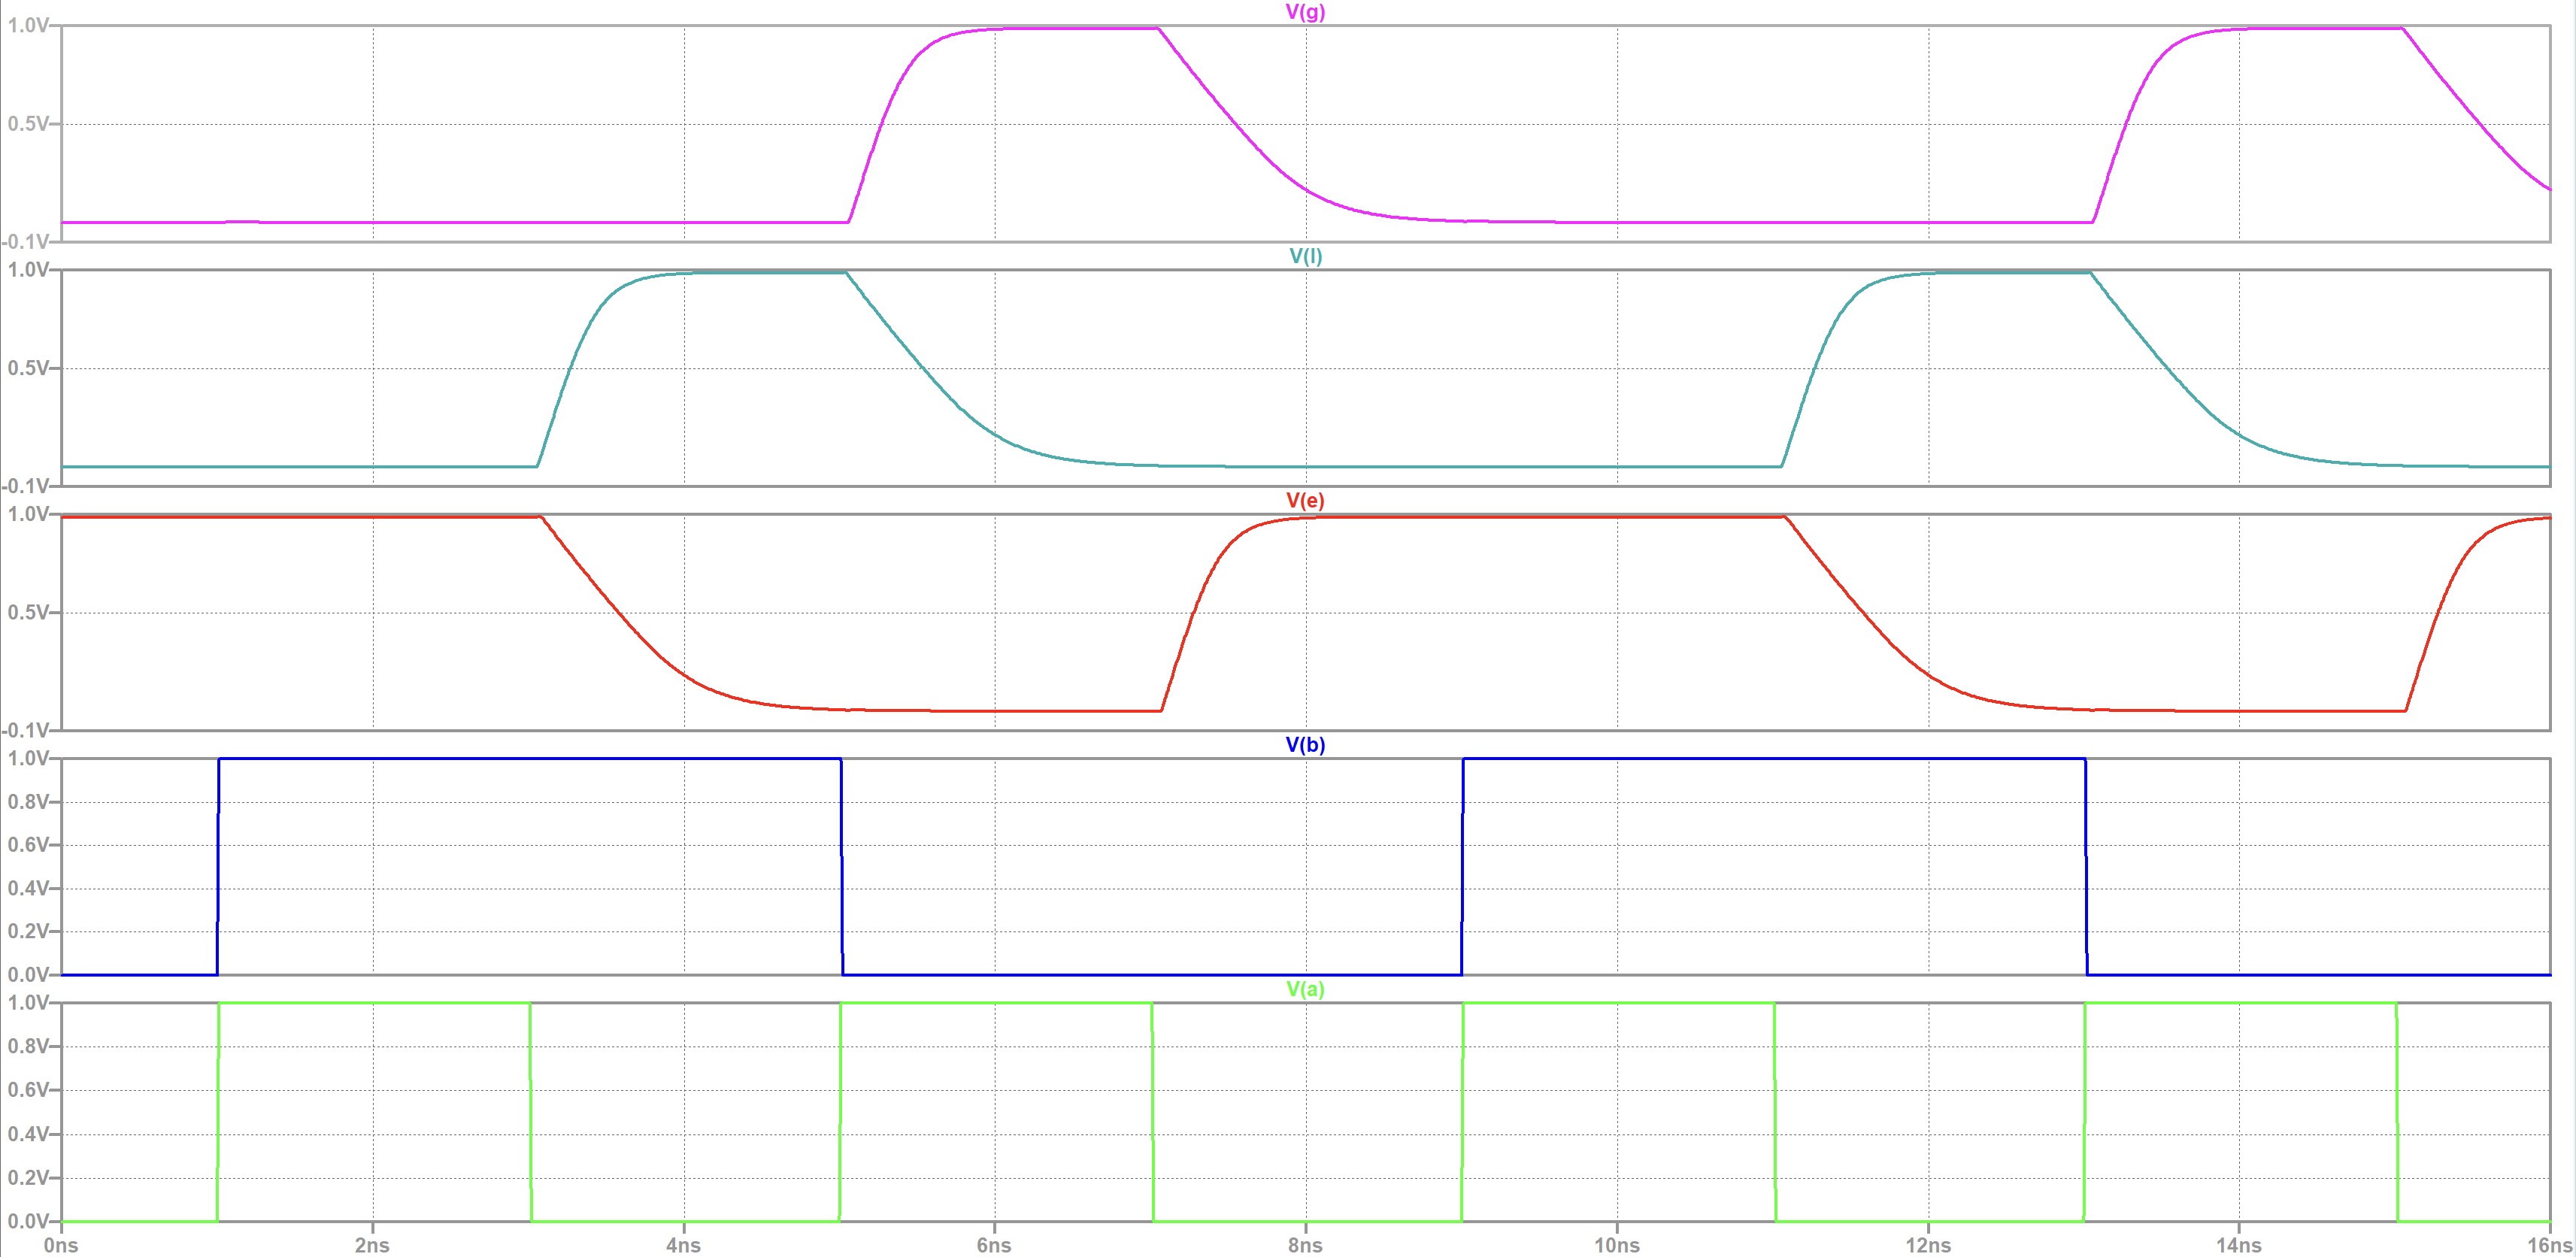
\includegraphics[width=\textwidth]{image/full-comparator1-test.png}
    \caption{Тестирование полного компаратора с двумя одноразрядными входами} 
\end{figure}

Чтобы уменьшить количество обозначений на схеме, сделаем символ полного компаратора с двумя одноразрядными входами
\begin{figure}[H]
    \centering
    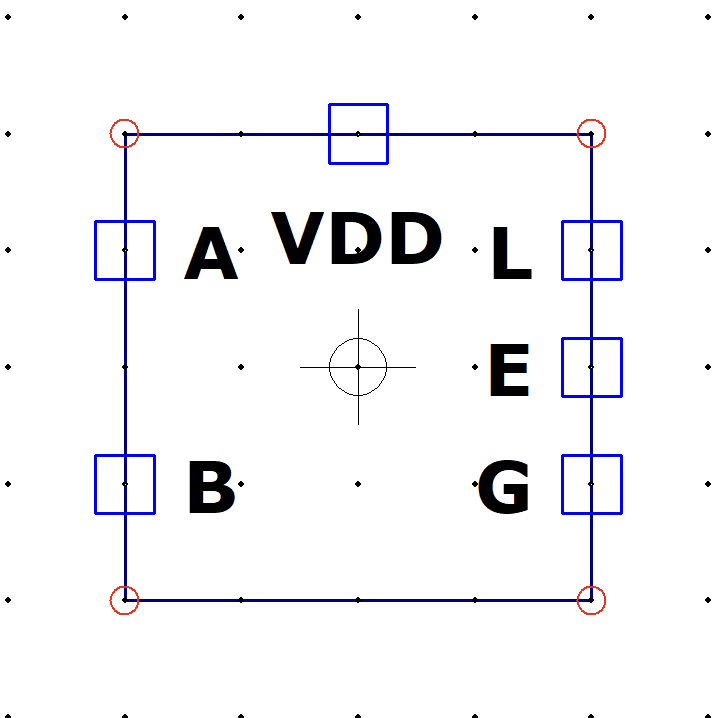
\includegraphics[width=0.3\textwidth]{image/full-comparator1-sym.png}
    \caption{Символ полного компаратора с двумя одноразрядными входами}
\end{figure}
Будем делать последовательный компаратор, поэтому добавим входы наращивания разрядности.
$$A\wedge B = (A \mid B) \mid (A \mid B)$$
$$A \vee B = (A \mid A) \mid (B \mid B)$$
\begin{figure}
    \centering
    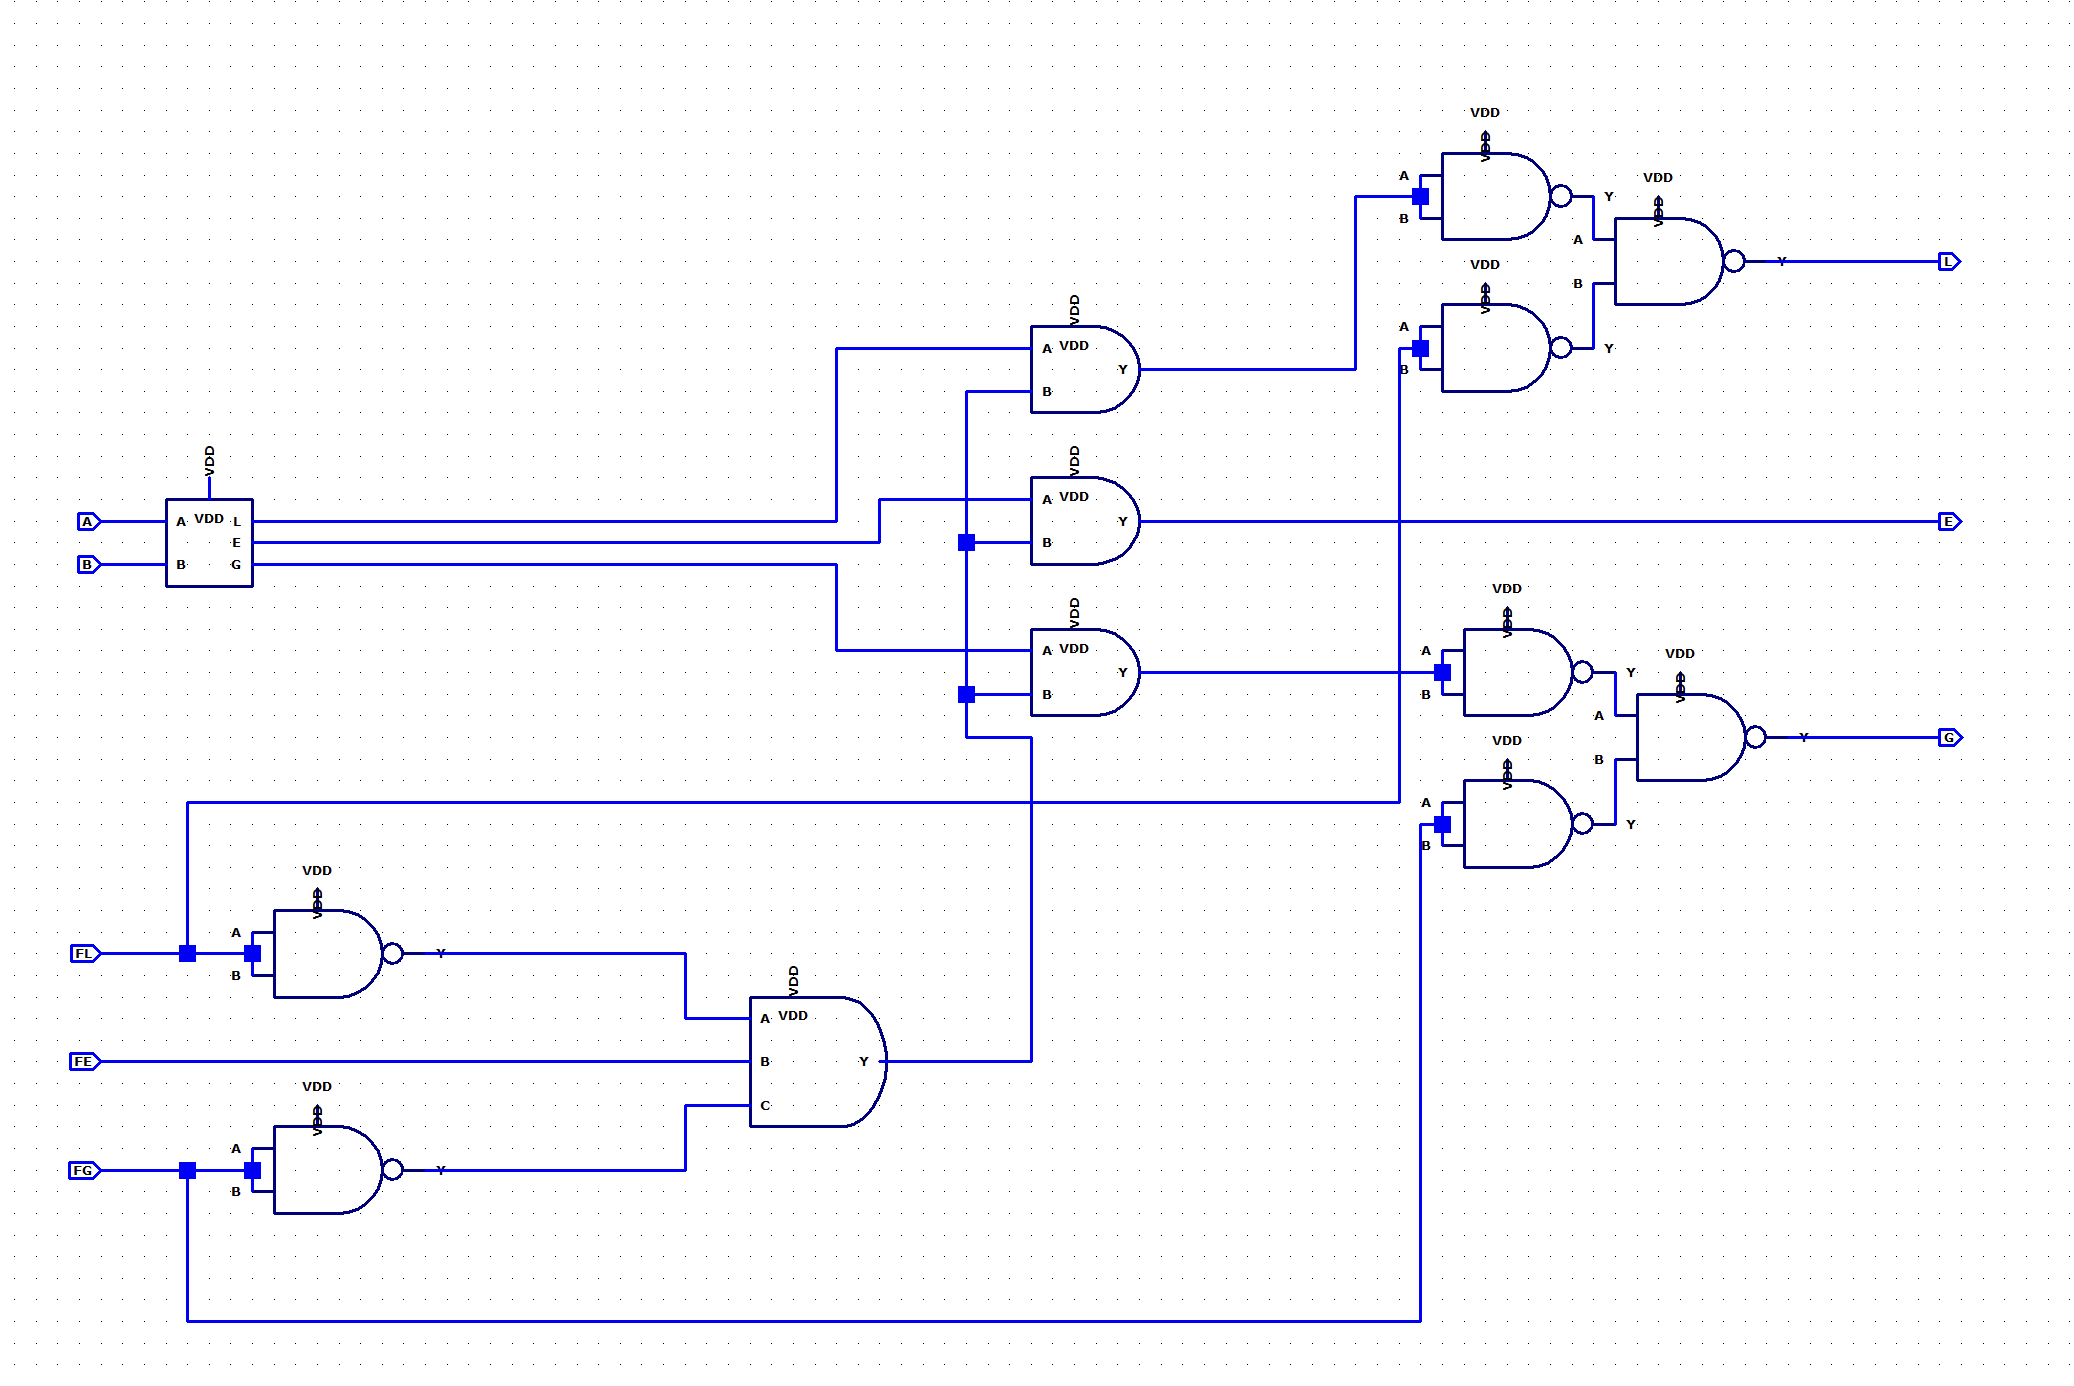
\includegraphics[width=\textwidth]{image/full-comparator-seq.png}
    \caption{Схема полного компаратора с двумя одноразрядными входами и входами наращивания разрядности}
\end{figure}
Чтобы не пугать людей, сделаем ещё символ для полного компаратора с двумя одноразрядными входами и входами наращивания разрядности:
\begin{figure}[H]
    \centering
    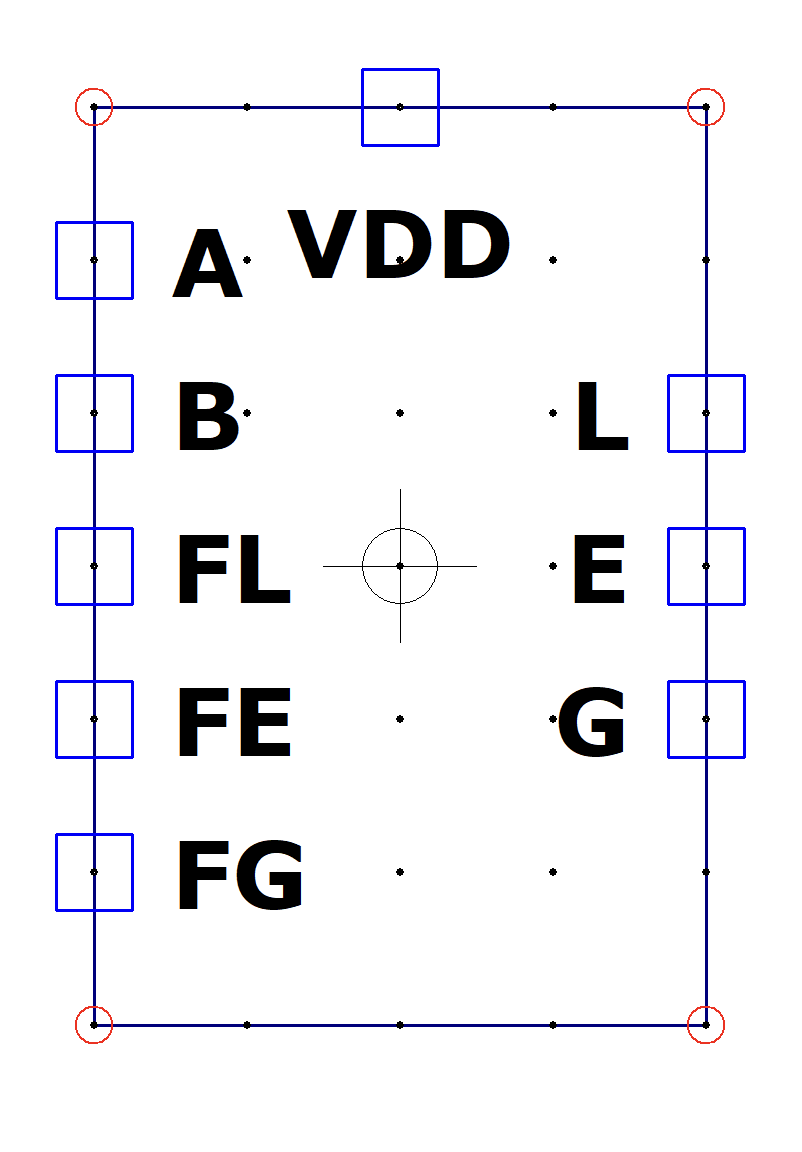
\includegraphics[width=0.3\textwidth]{image/full-comparator-seq-sym.png}
    \caption{Символ полного компаратора с двумя одноразрядными входами и входами наращивания разрядности}
\end{figure}
Подключим компараторы в последовательную цепочку, чтобы получить полный четырехразрядный компаратор.
Насладимся красатой получившейся схемы, не забывая про тестирование на каждом из этапов.
\begin{figure}[H]
    \centering
    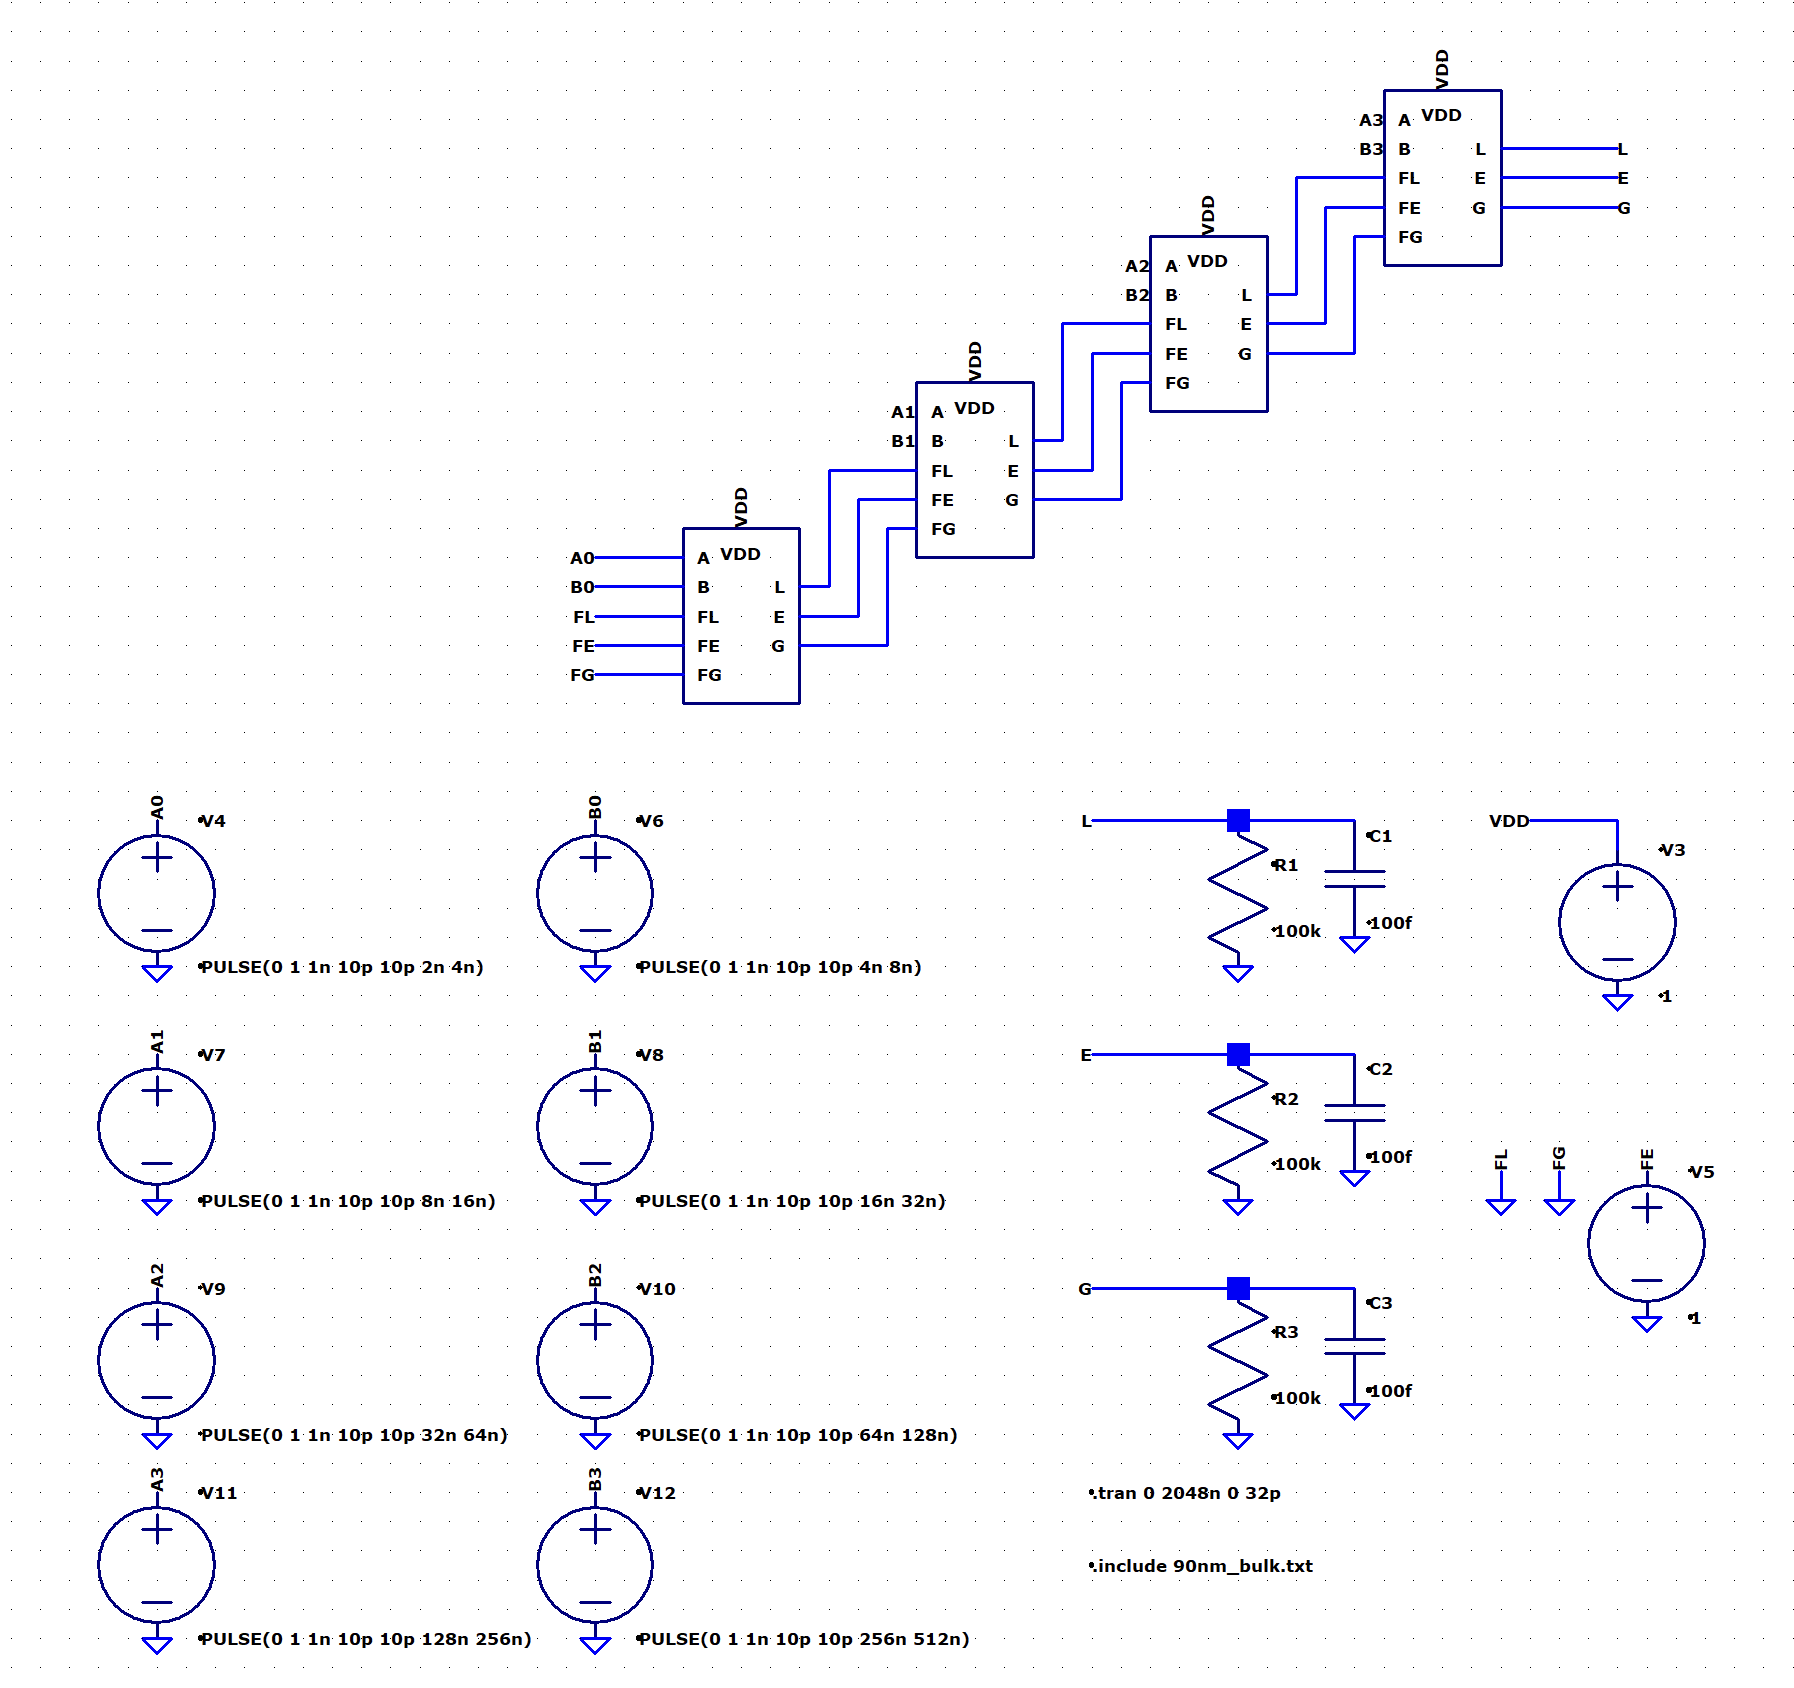
\includegraphics[width=\textwidth]{image/full-comparator.png}
    \caption{Схема полного четырехразрядного компаратора}
\end{figure}
\begin{figure}{H}
    \centering
    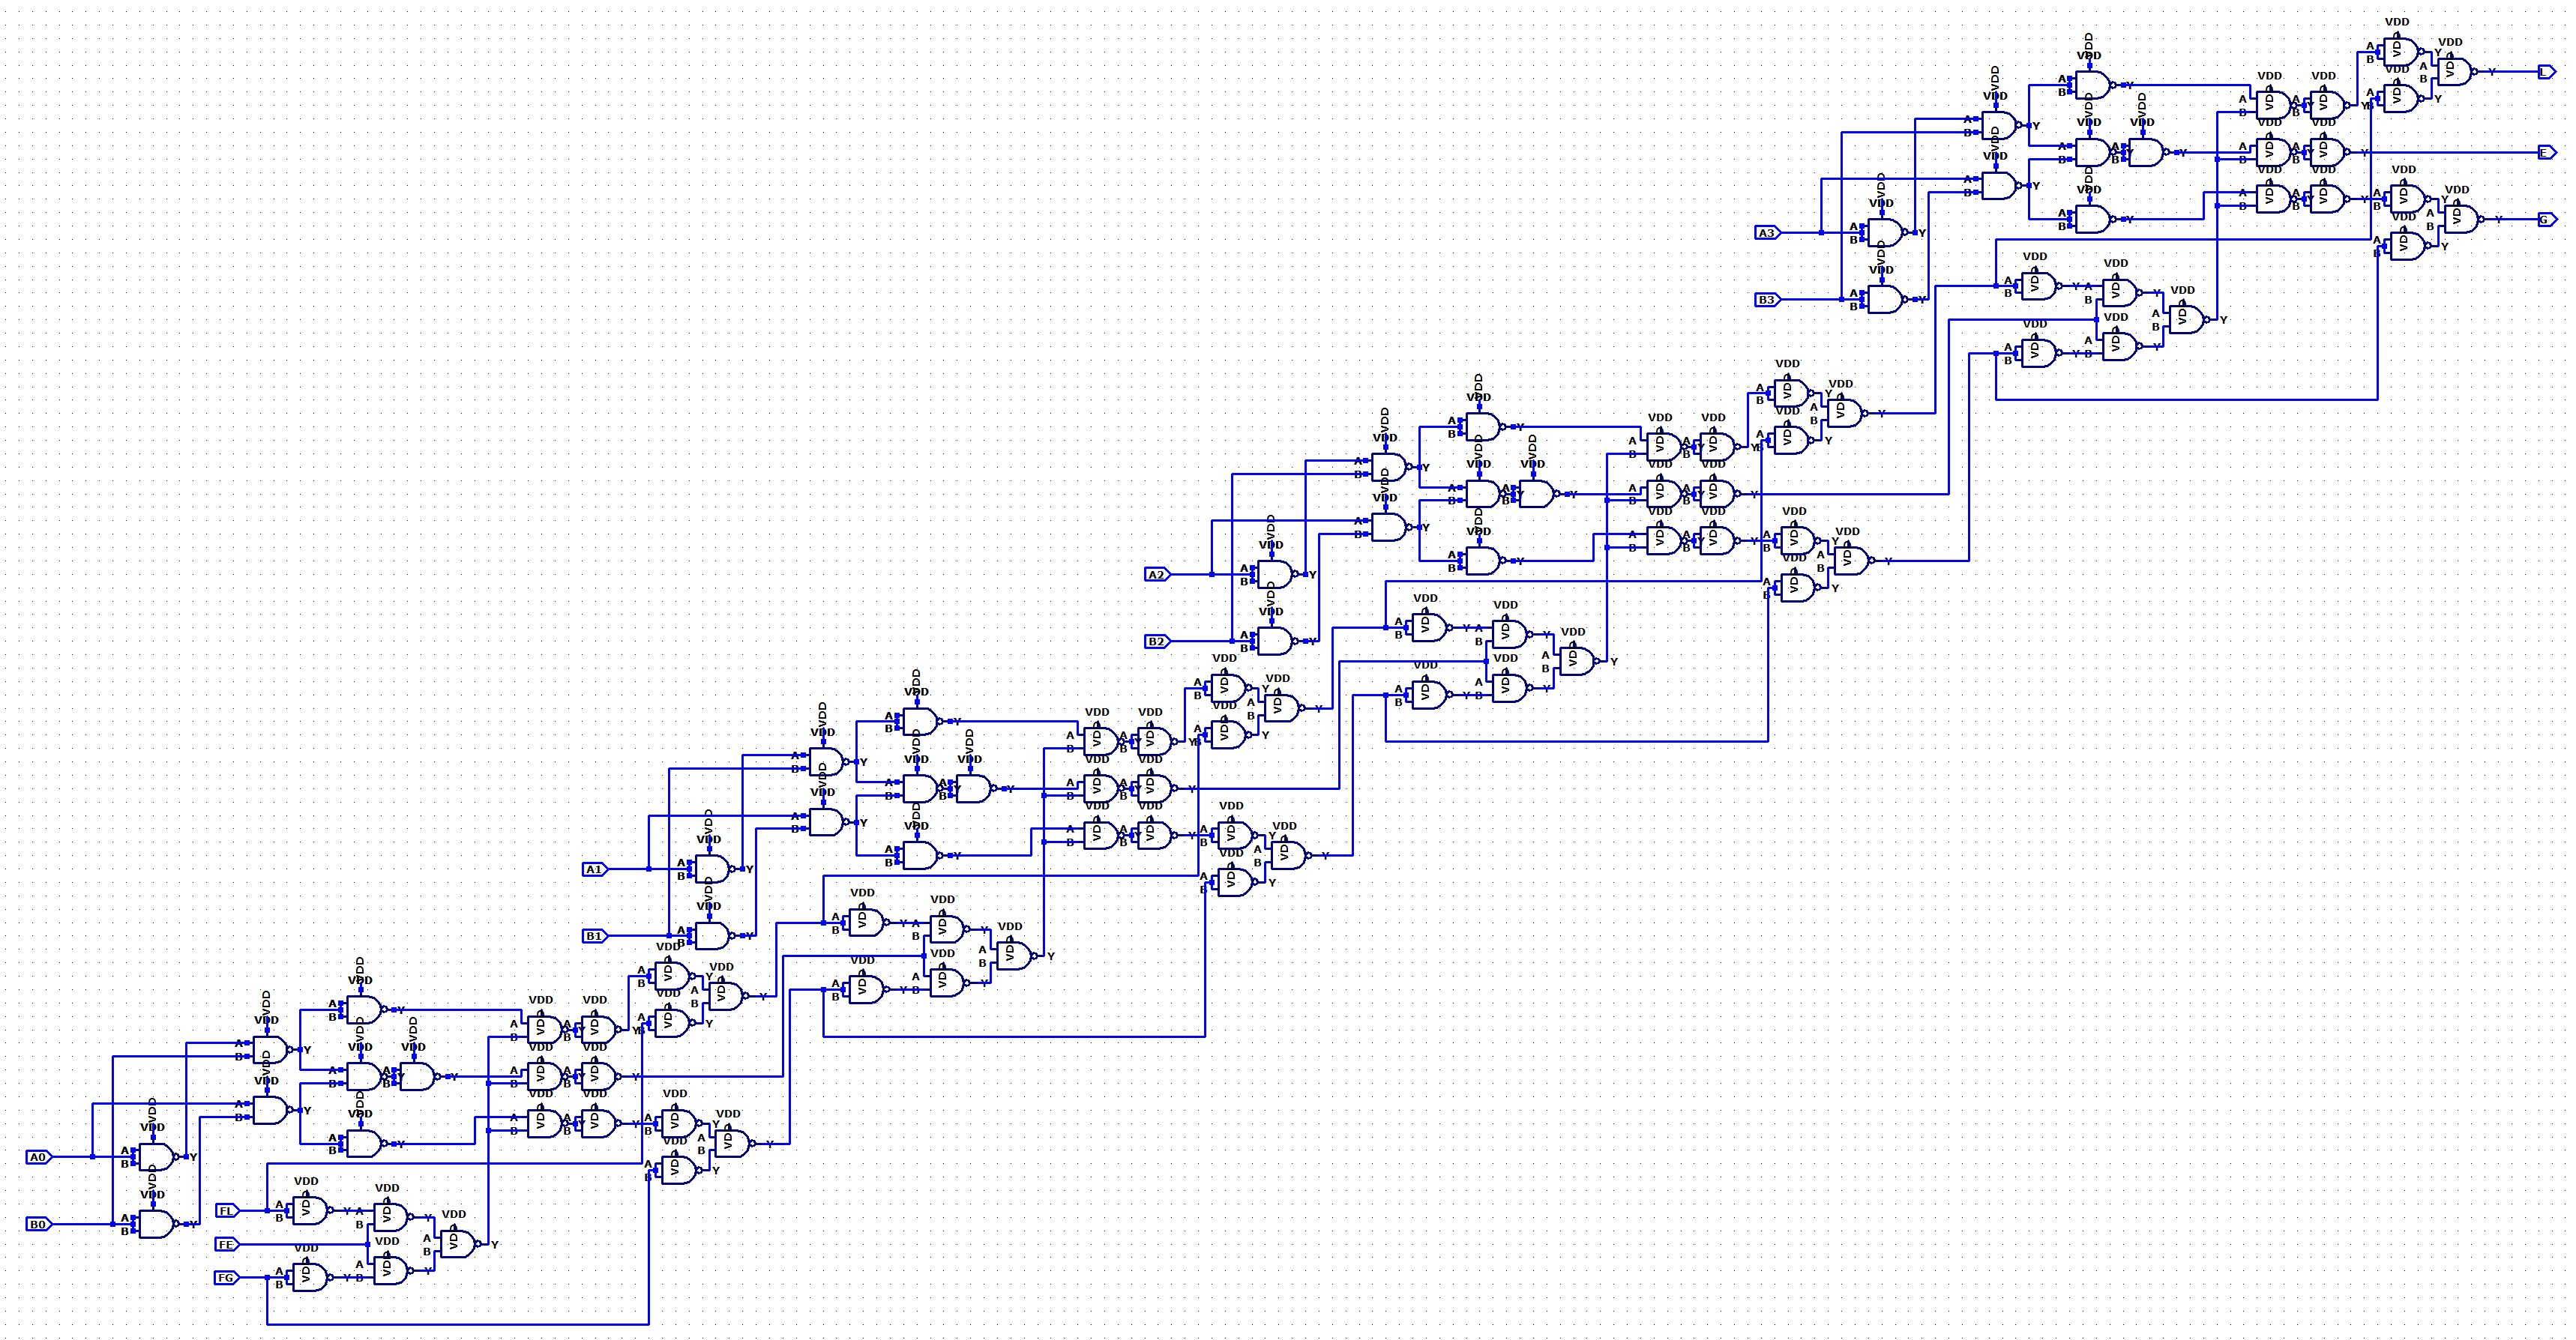
\includegraphics[width=\textwidth]{image/full-comparator4-all-in-one.png}
    \caption{Тоже самое, но без вспомагательных символов. Слабонервным не смотреть) }
\end{figure}
\subsection{Создайте символ для построенного БОЭ.}
\begin{figure}[H]
    \centering
    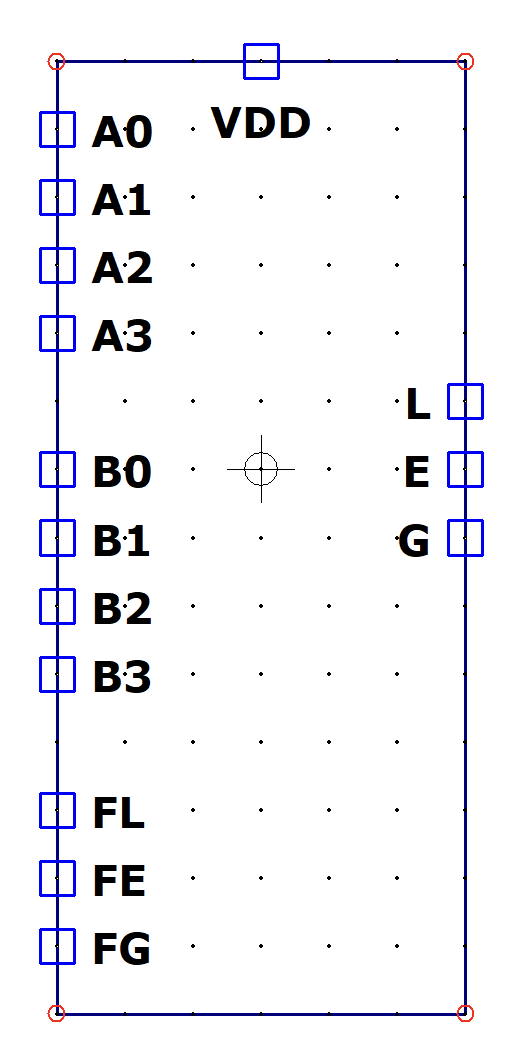
\includegraphics[width=0.3\textwidth]{image/full-comparator-sym.png}
    \caption{Символ полного четырехразрядного компаратора}
\end{figure}
\subsection{Проведите моделирование работы схемы и определите задержку распространения сигнала через БОЭ.}
\begin{figure}[H]
    \centering
    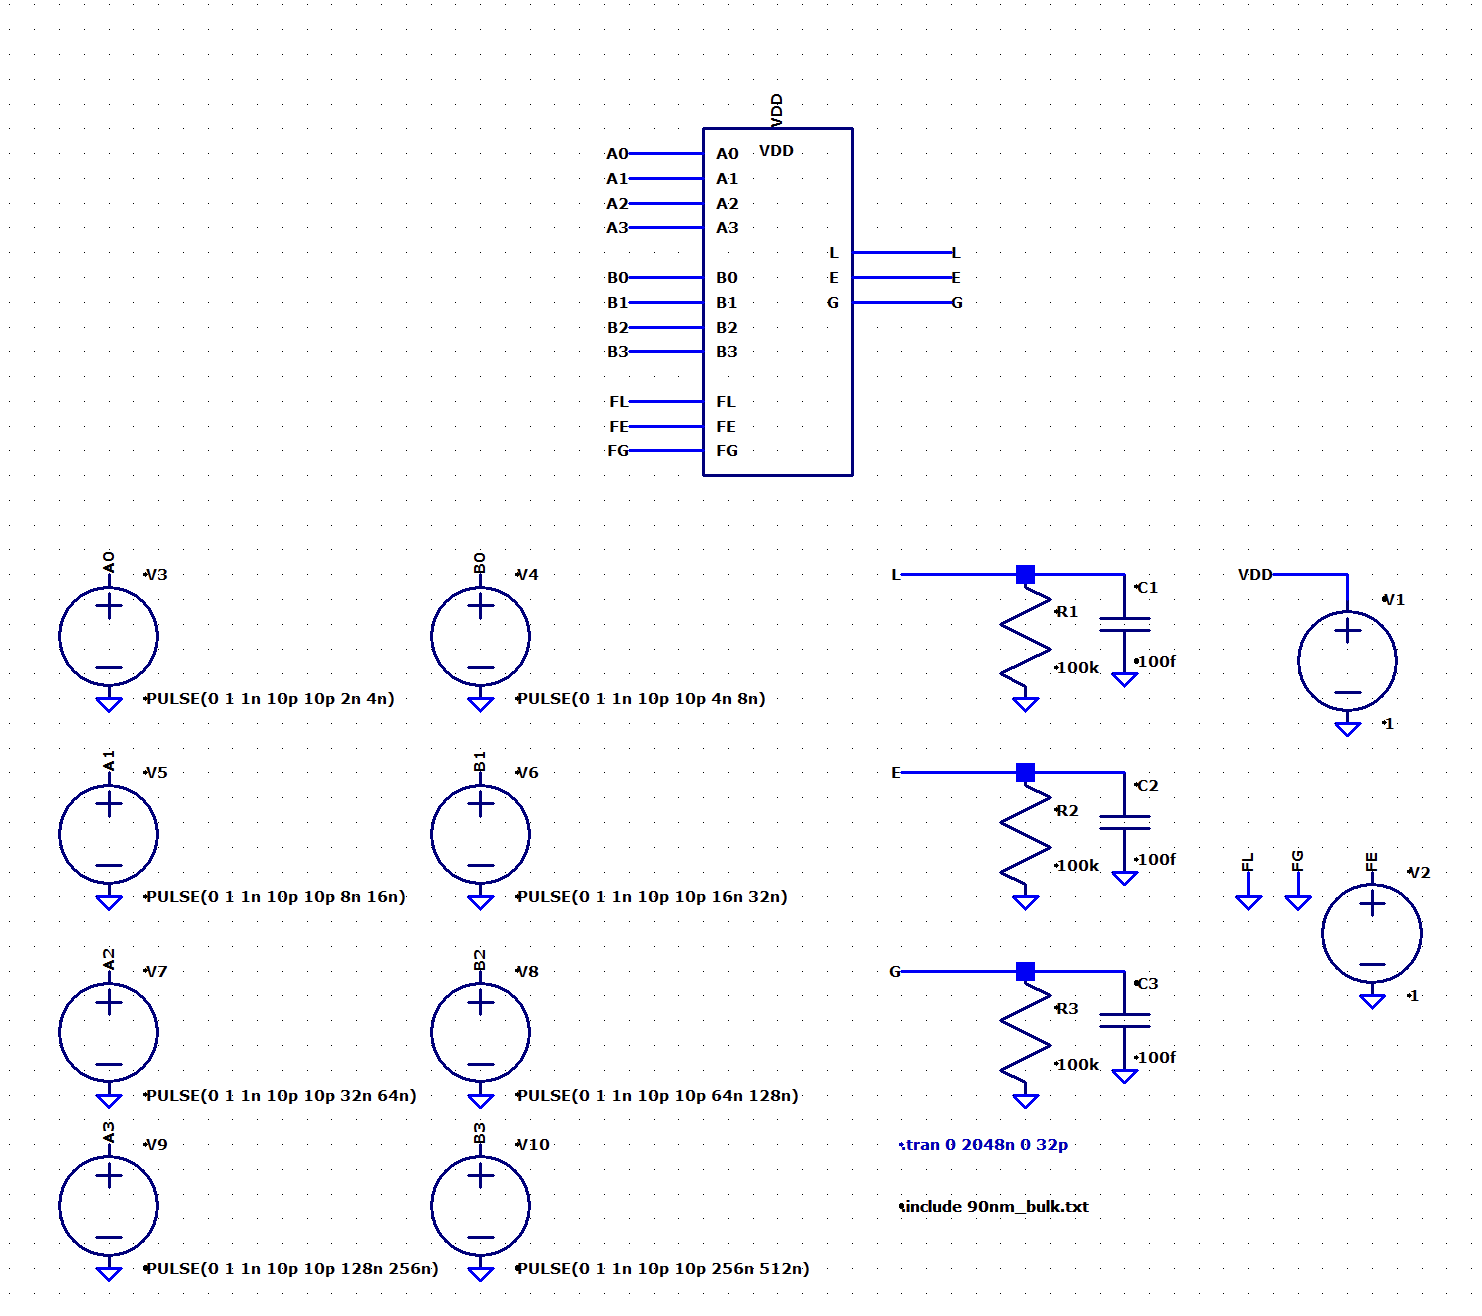
\includegraphics[width=\textwidth]{image/full-comparator-test-env.png}
    \caption{Схема тестирование полного четырехразрядного компаратора}
\end{figure}
\begin{figure}[H]
    \centering
    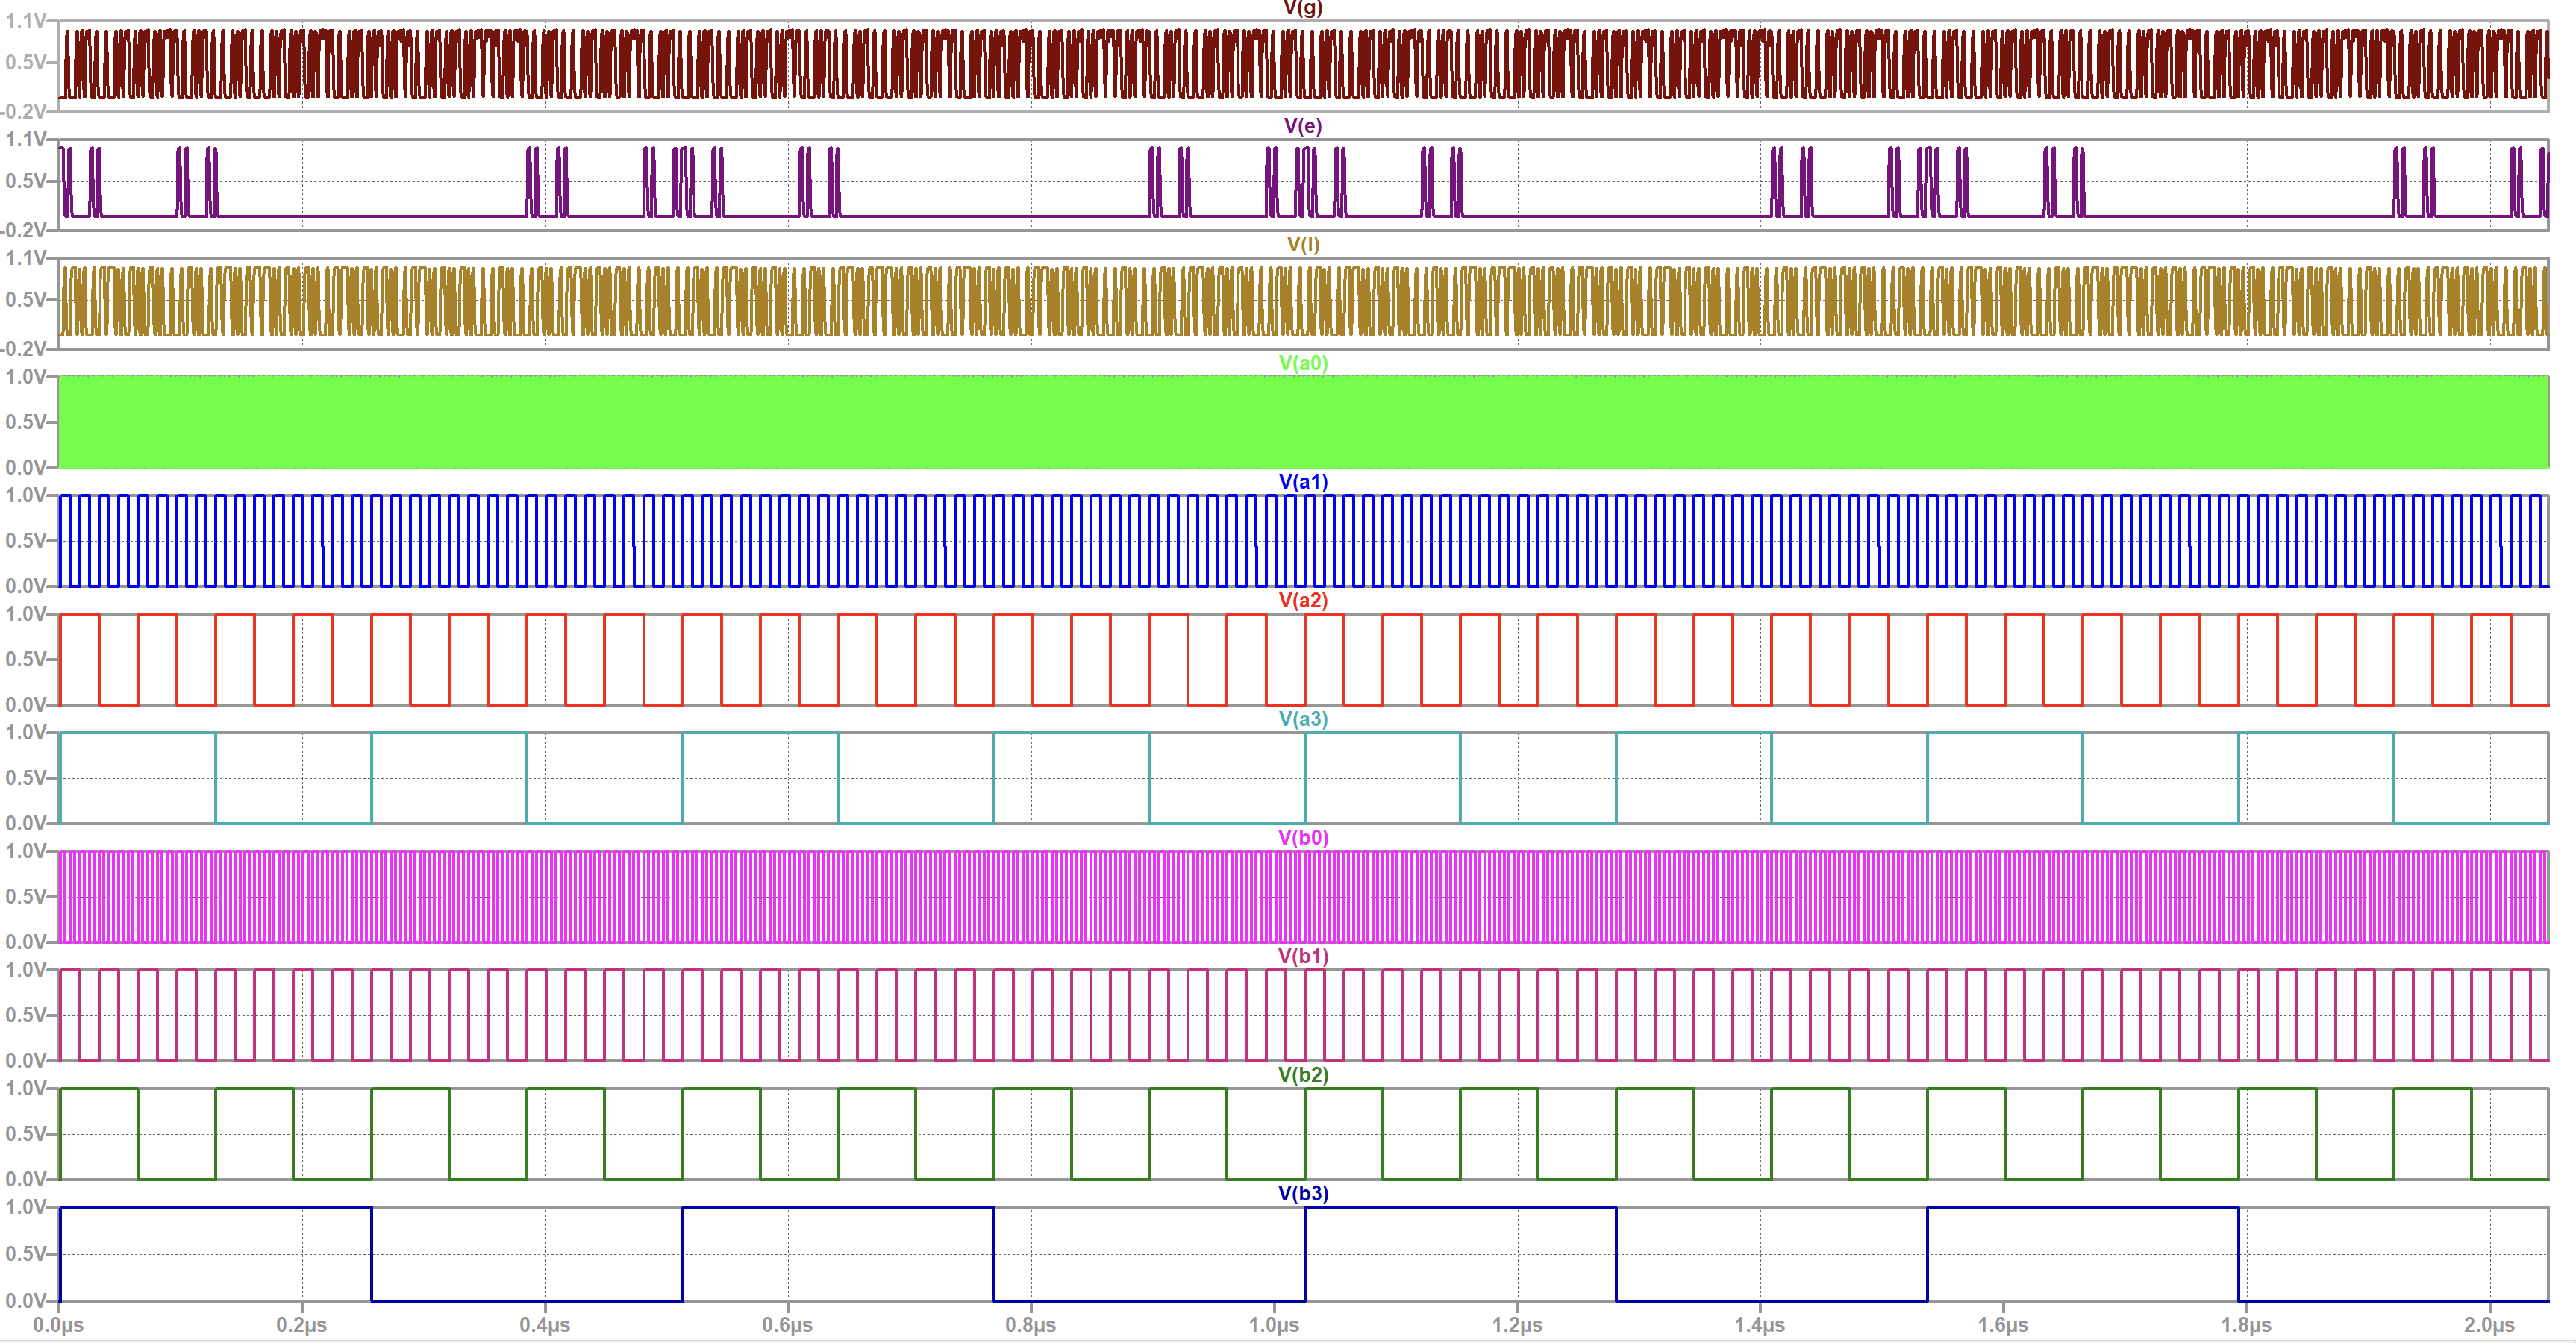
\includegraphics[width=\textwidth]{image/full-comparator-test-all-states.png}
    \caption{Все возможные состояния. Ничего не понятно, но очень интересно}
\end{figure}
\begin{figure}[H]
    \centering
    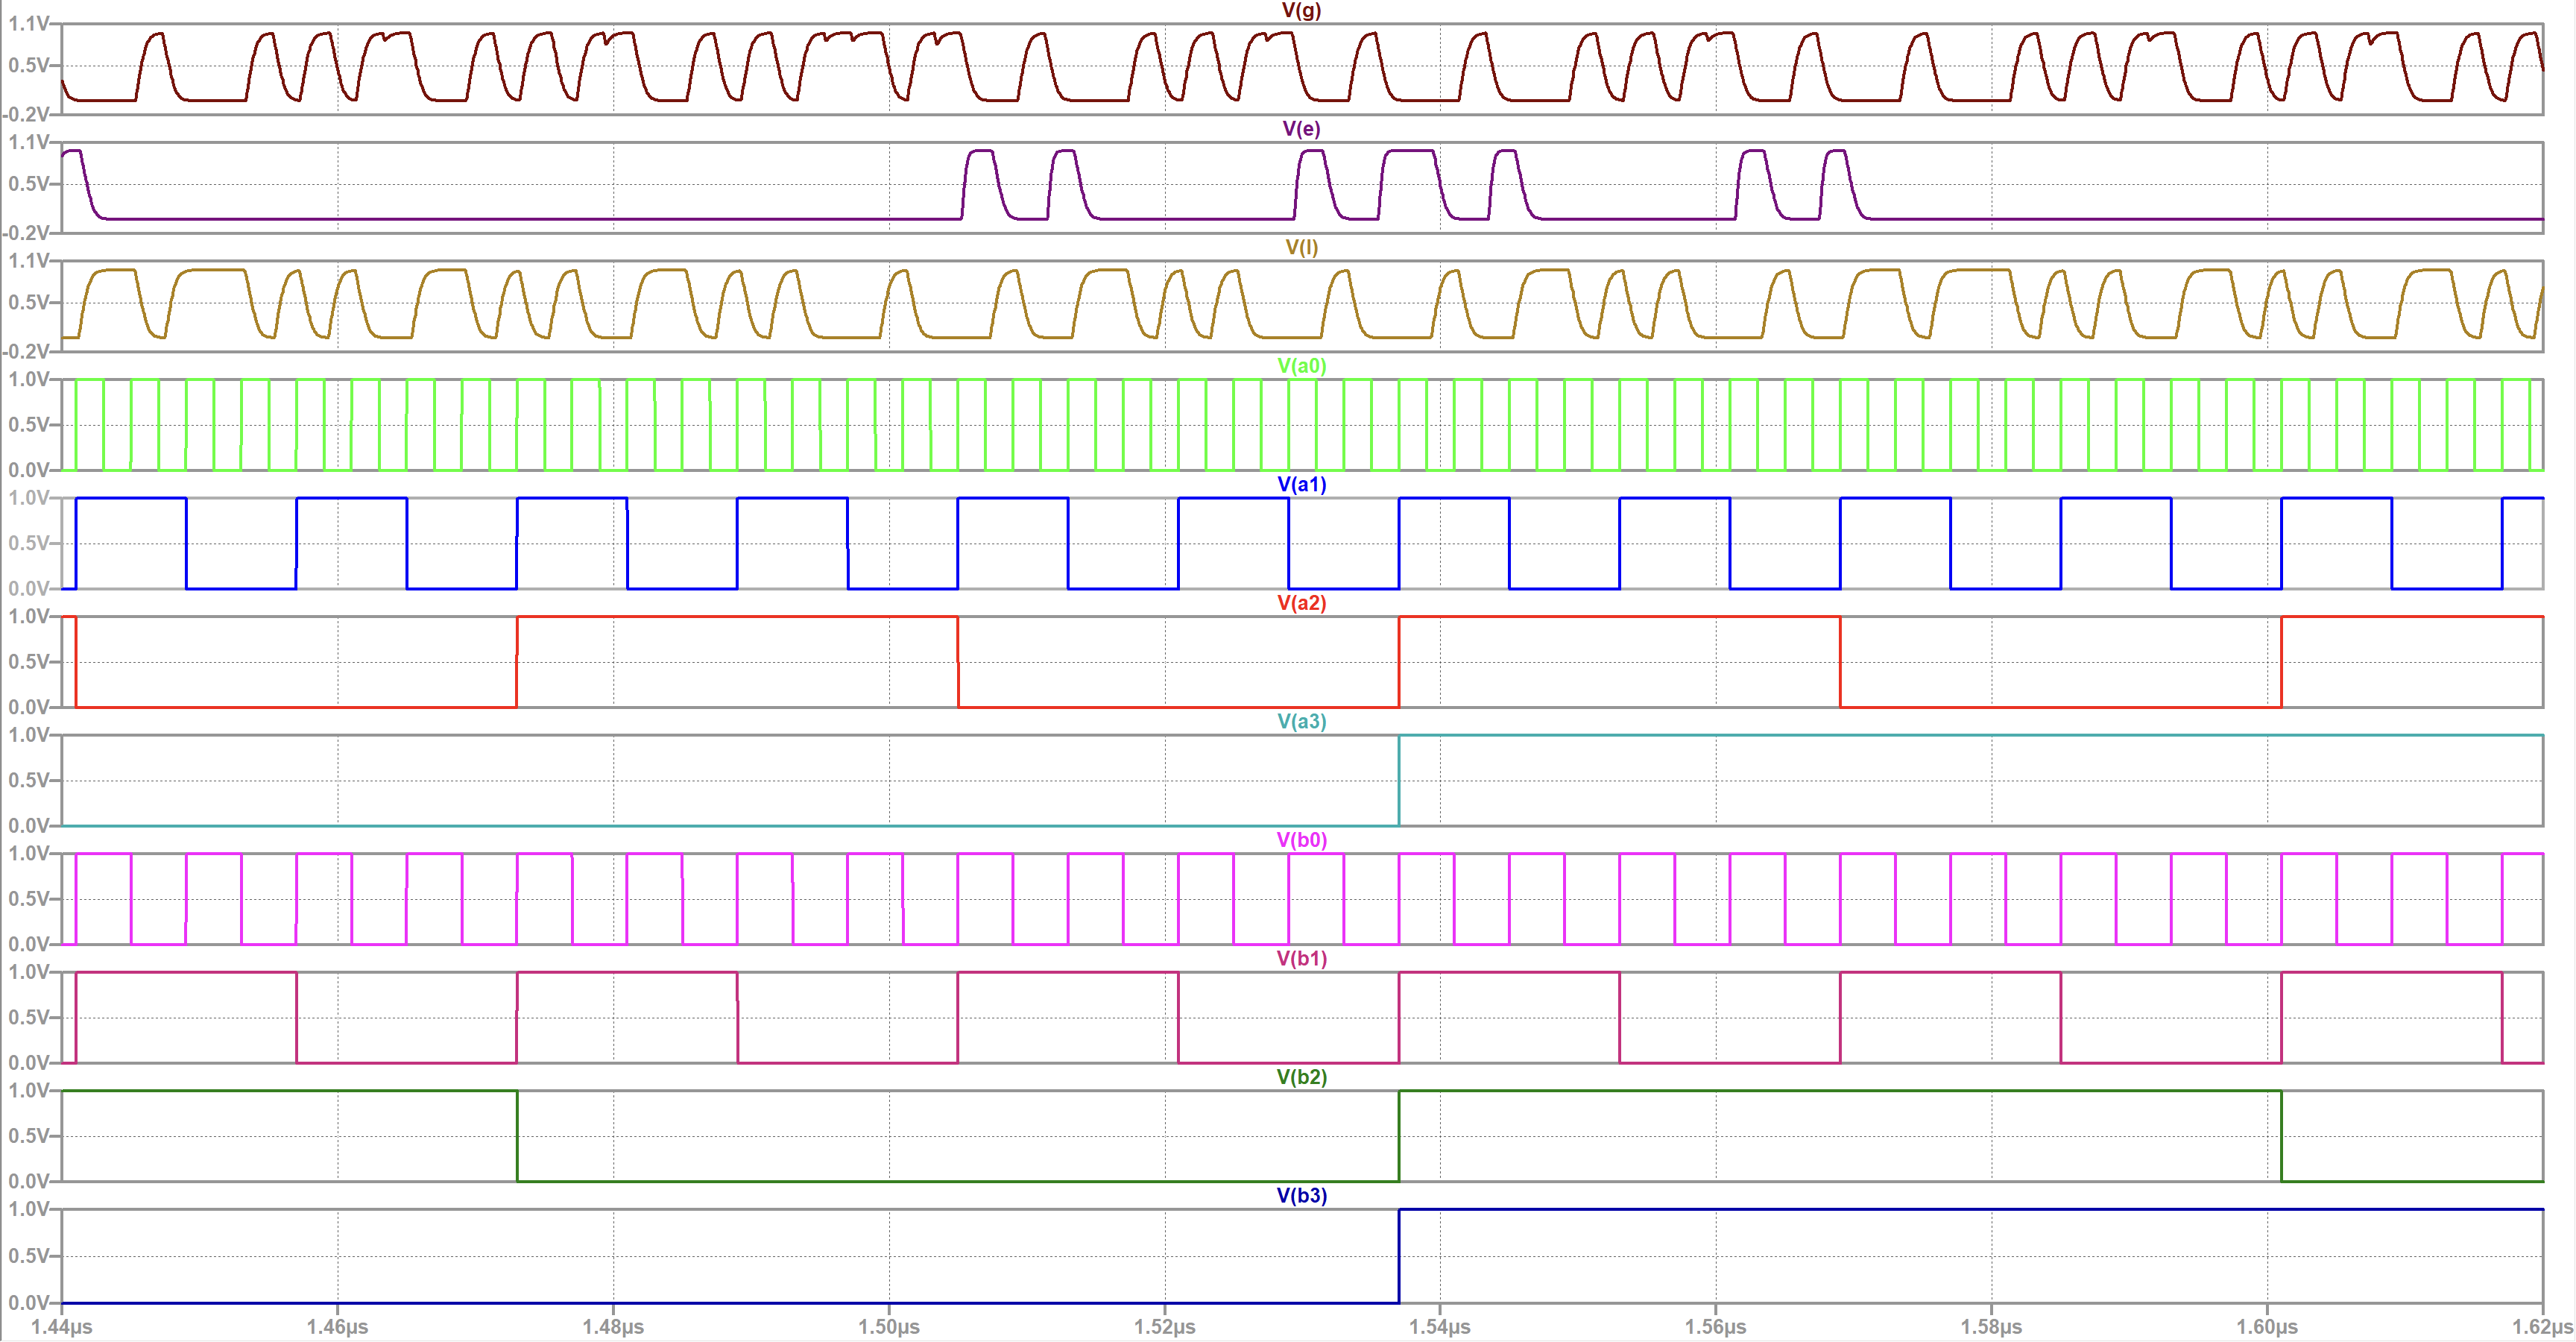
\includegraphics[width=\textwidth]{image/full-comparator-test-zoom.png}
    \caption{Рассмотрим поближе. Видим, что компаратор выдает верные значения}
\end{figure}
\subsection{Результат измерения задержки распространения сигнала через БОЭ}
\begin{figure}[H]
    \centering
    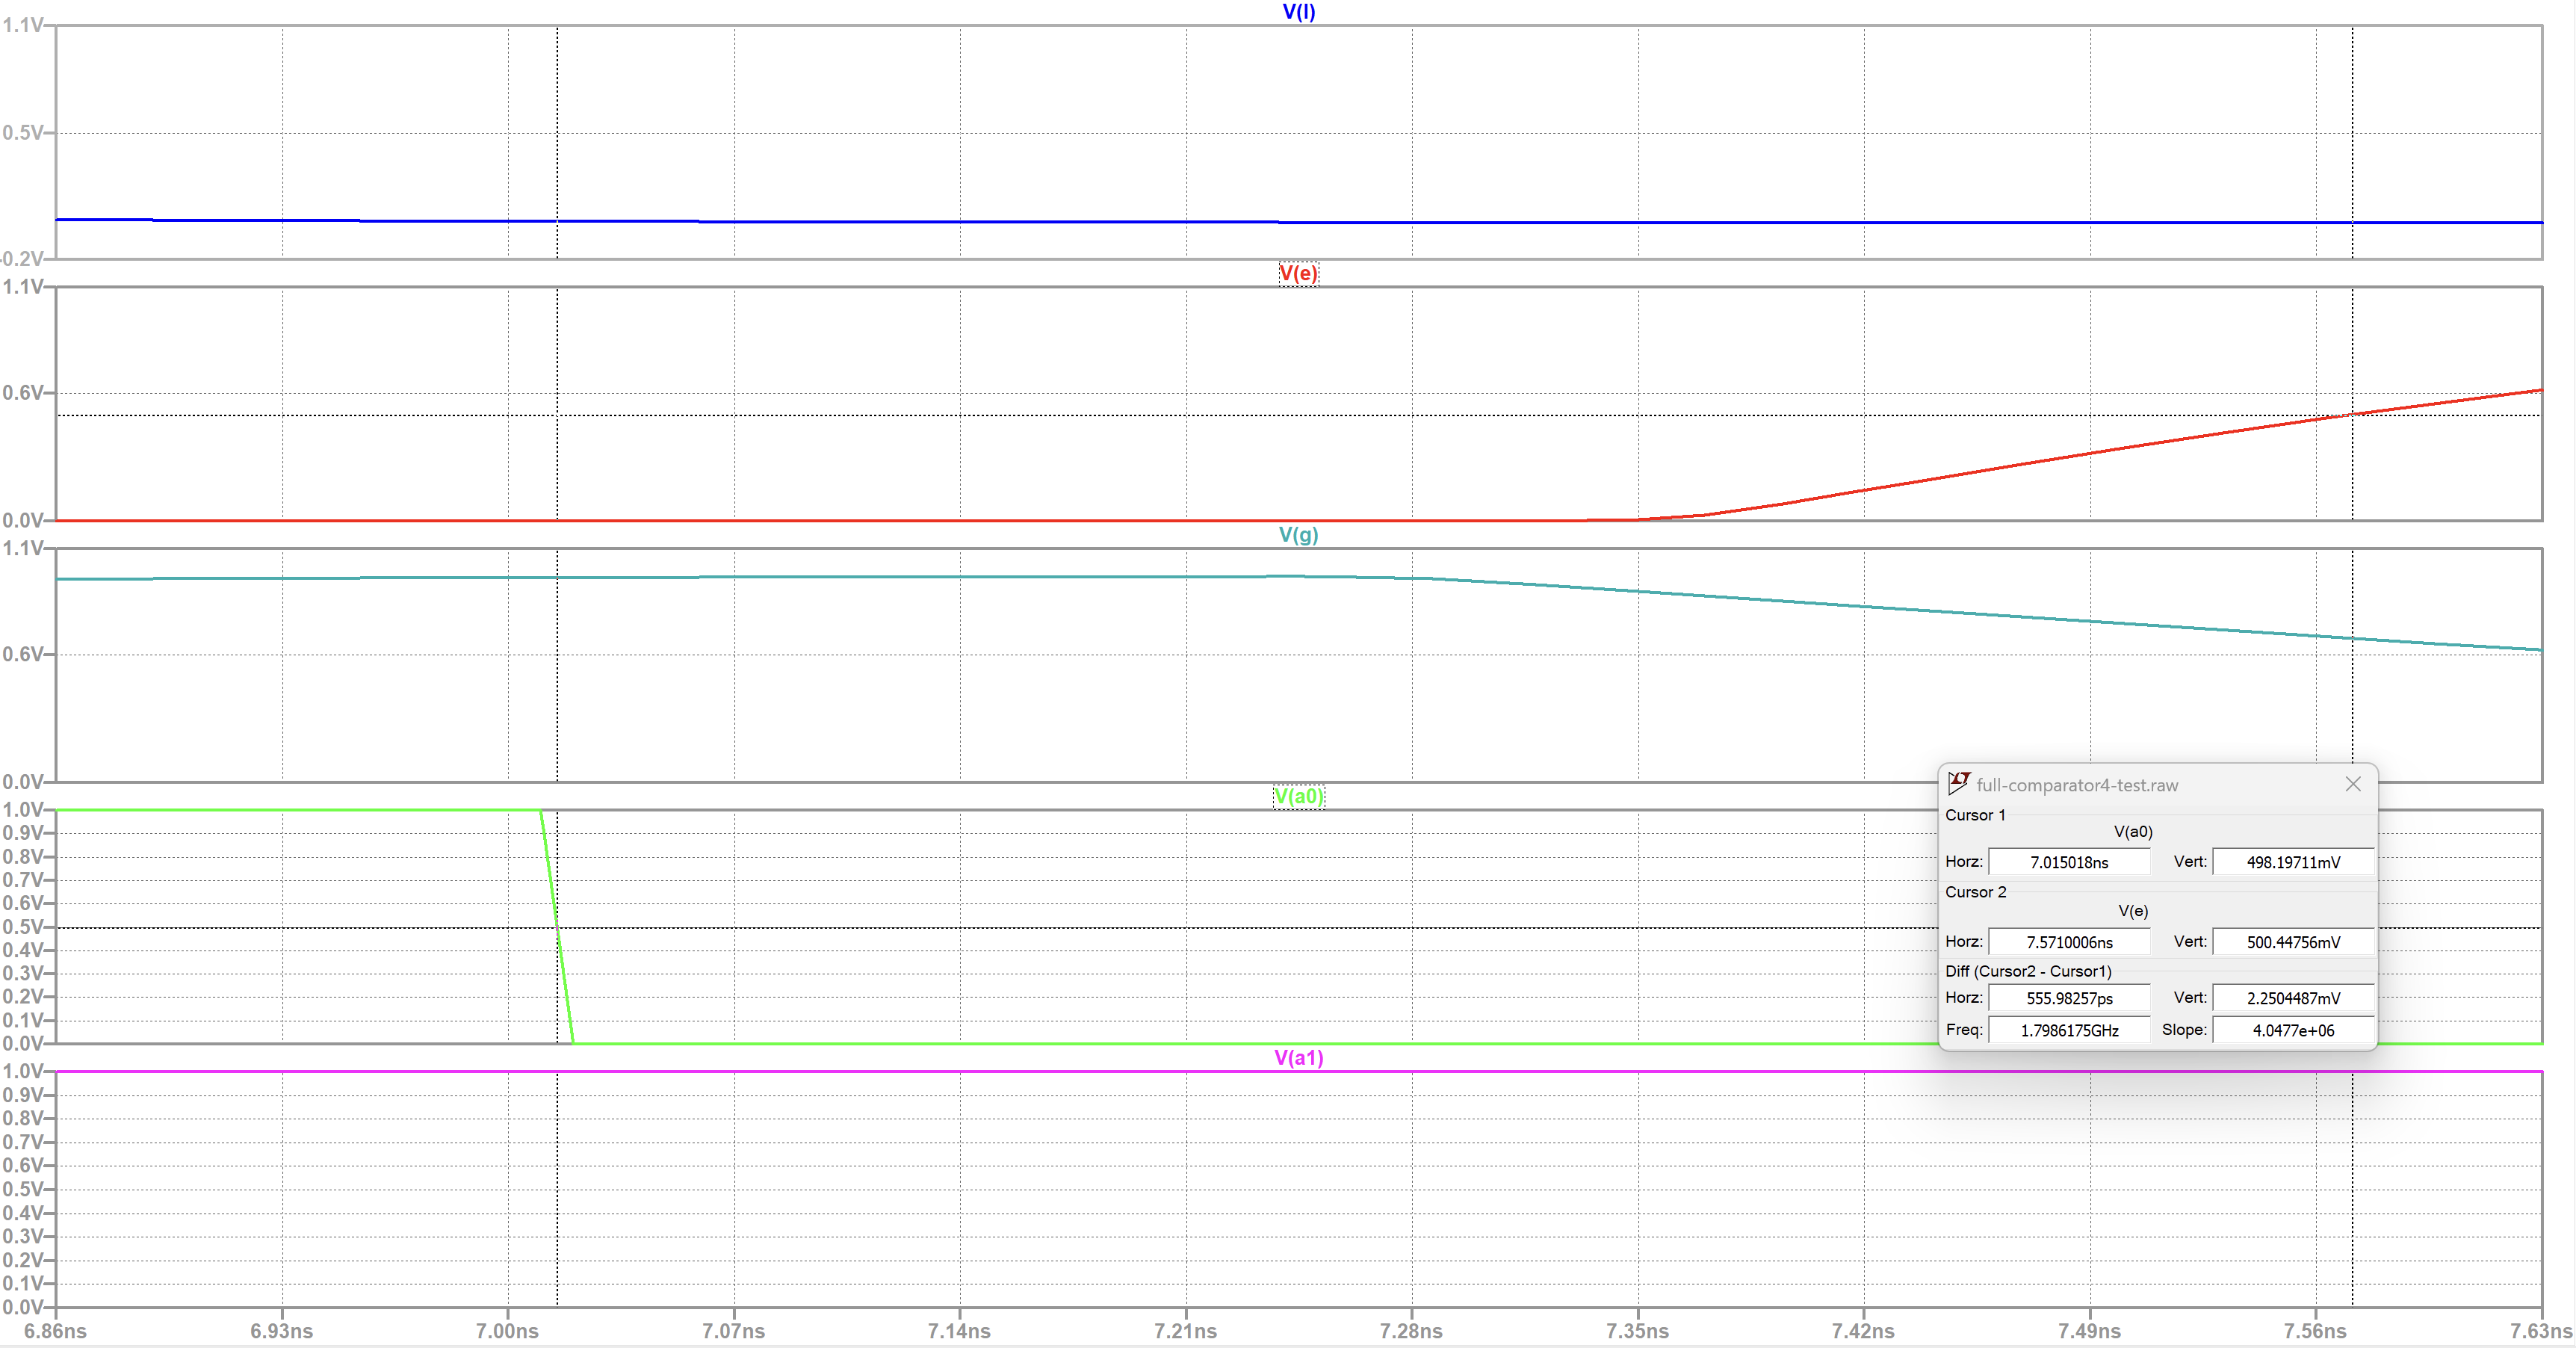
\includegraphics[width=\textwidth]{image/full-comparator-test-eq-01.png}
    \caption{Подсчет задержки распространения сигнала для 0-1 на выходе equal}
\end{figure}

$$t_{\text{pd}} = 7.571 - 7.015 = 0.556 ns$$
\begin{figure}[H]
    \centering
    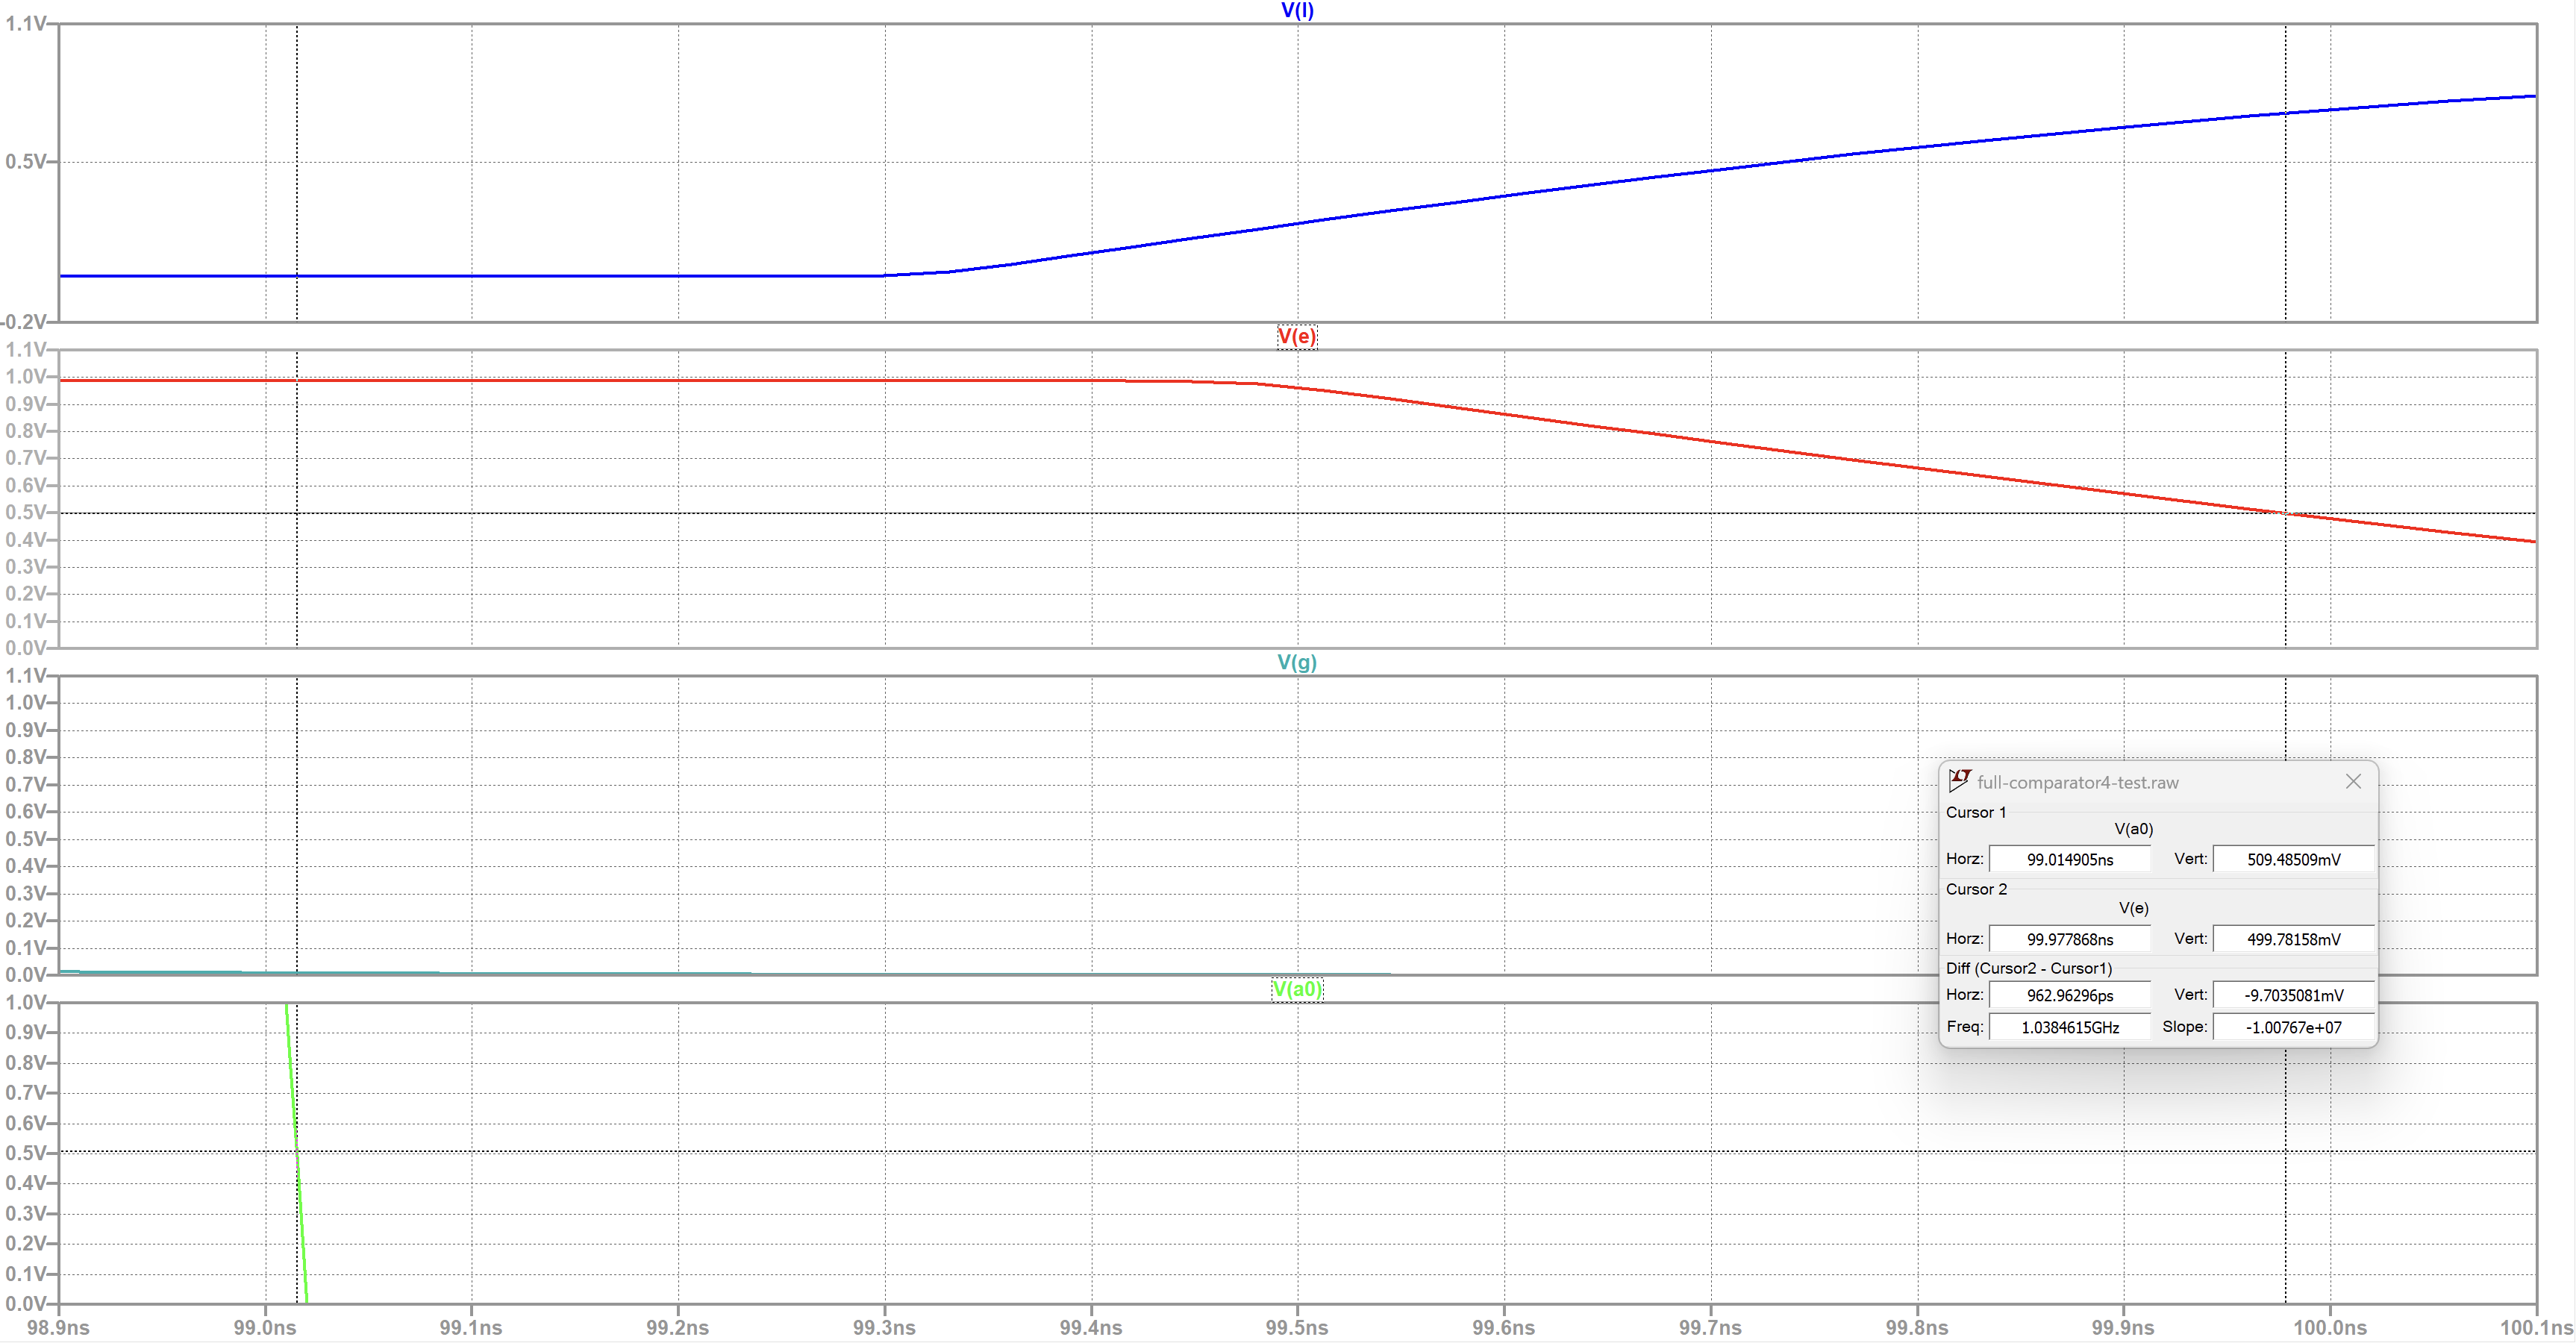
\includegraphics[width=\textwidth]{image/full-comparator-test-eq-10.png}
    \caption{Подсчет задержки распространения сигнала для 1-0 на выходе equal}
\end{figure}
$$t_{\text{pd}} = 99.977 - 99.015 = 0.963 ns$$
\begin{figure}[H]
    \centering
    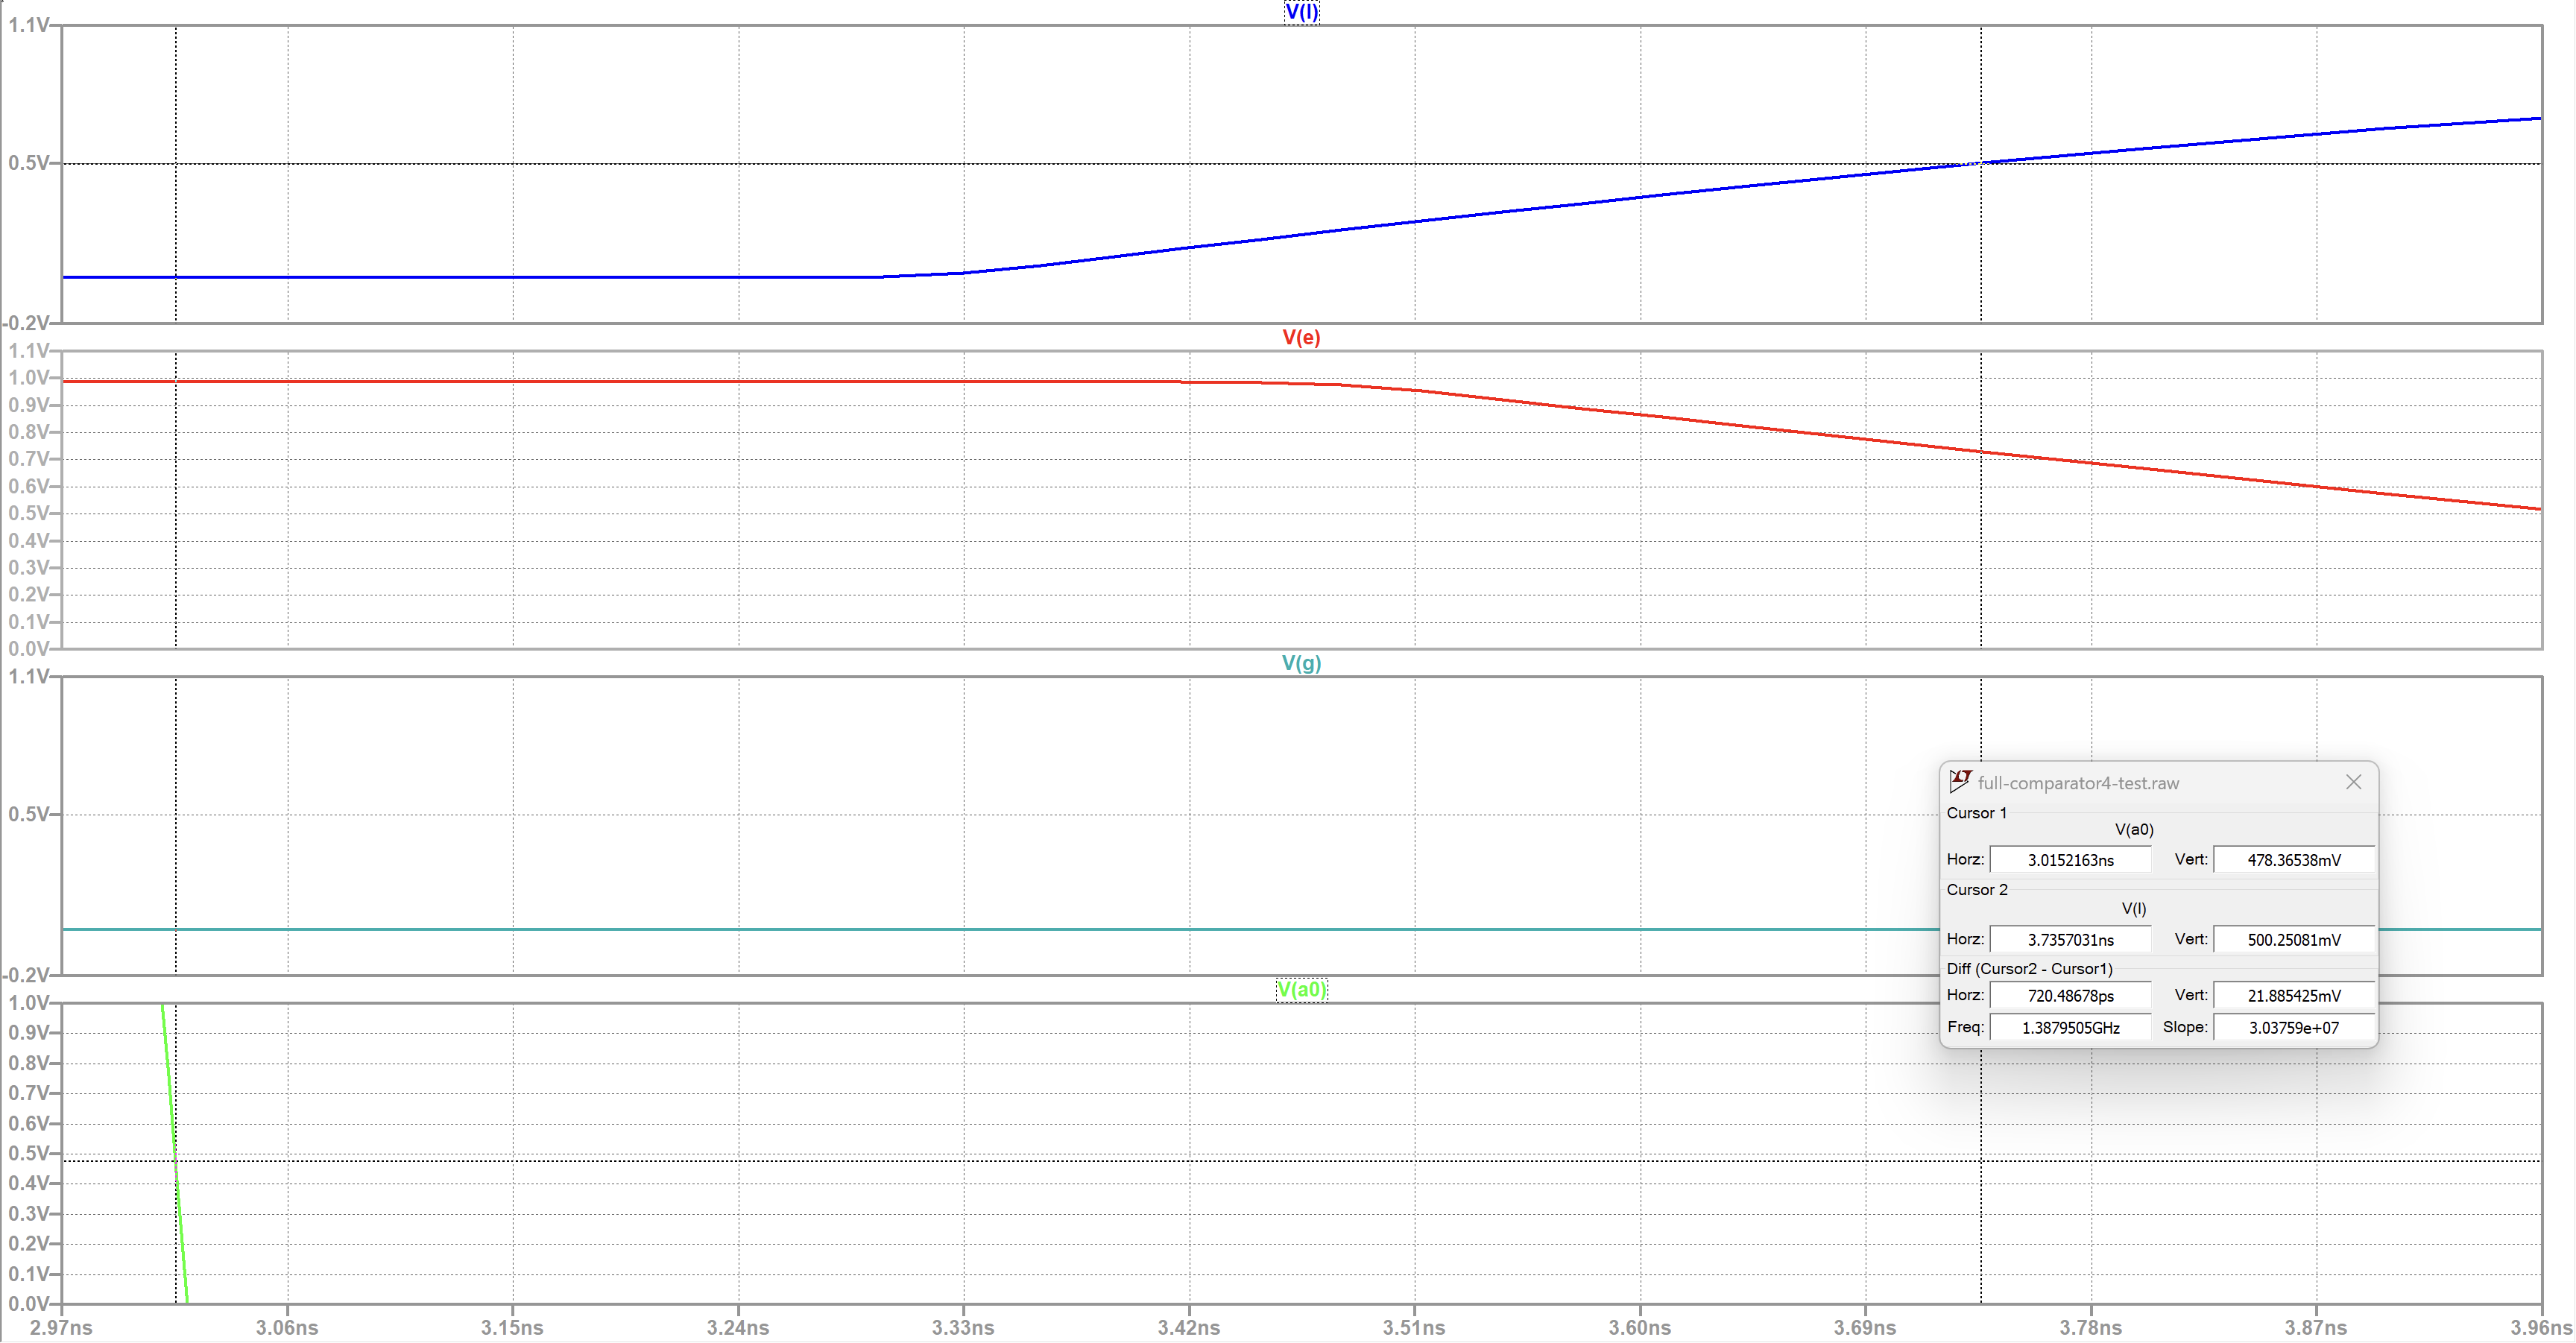
\includegraphics[width=\textwidth]{image/full-comparator-test-less-01.png}
    \caption{Подсчет задержки распространения сигнала для 0-1 на выходе less}
\end{figure}
$$t_{\text{pd}} = 3.736 - 3.015 = 0.720 ns$$
\begin{figure}[H]
    \centering
    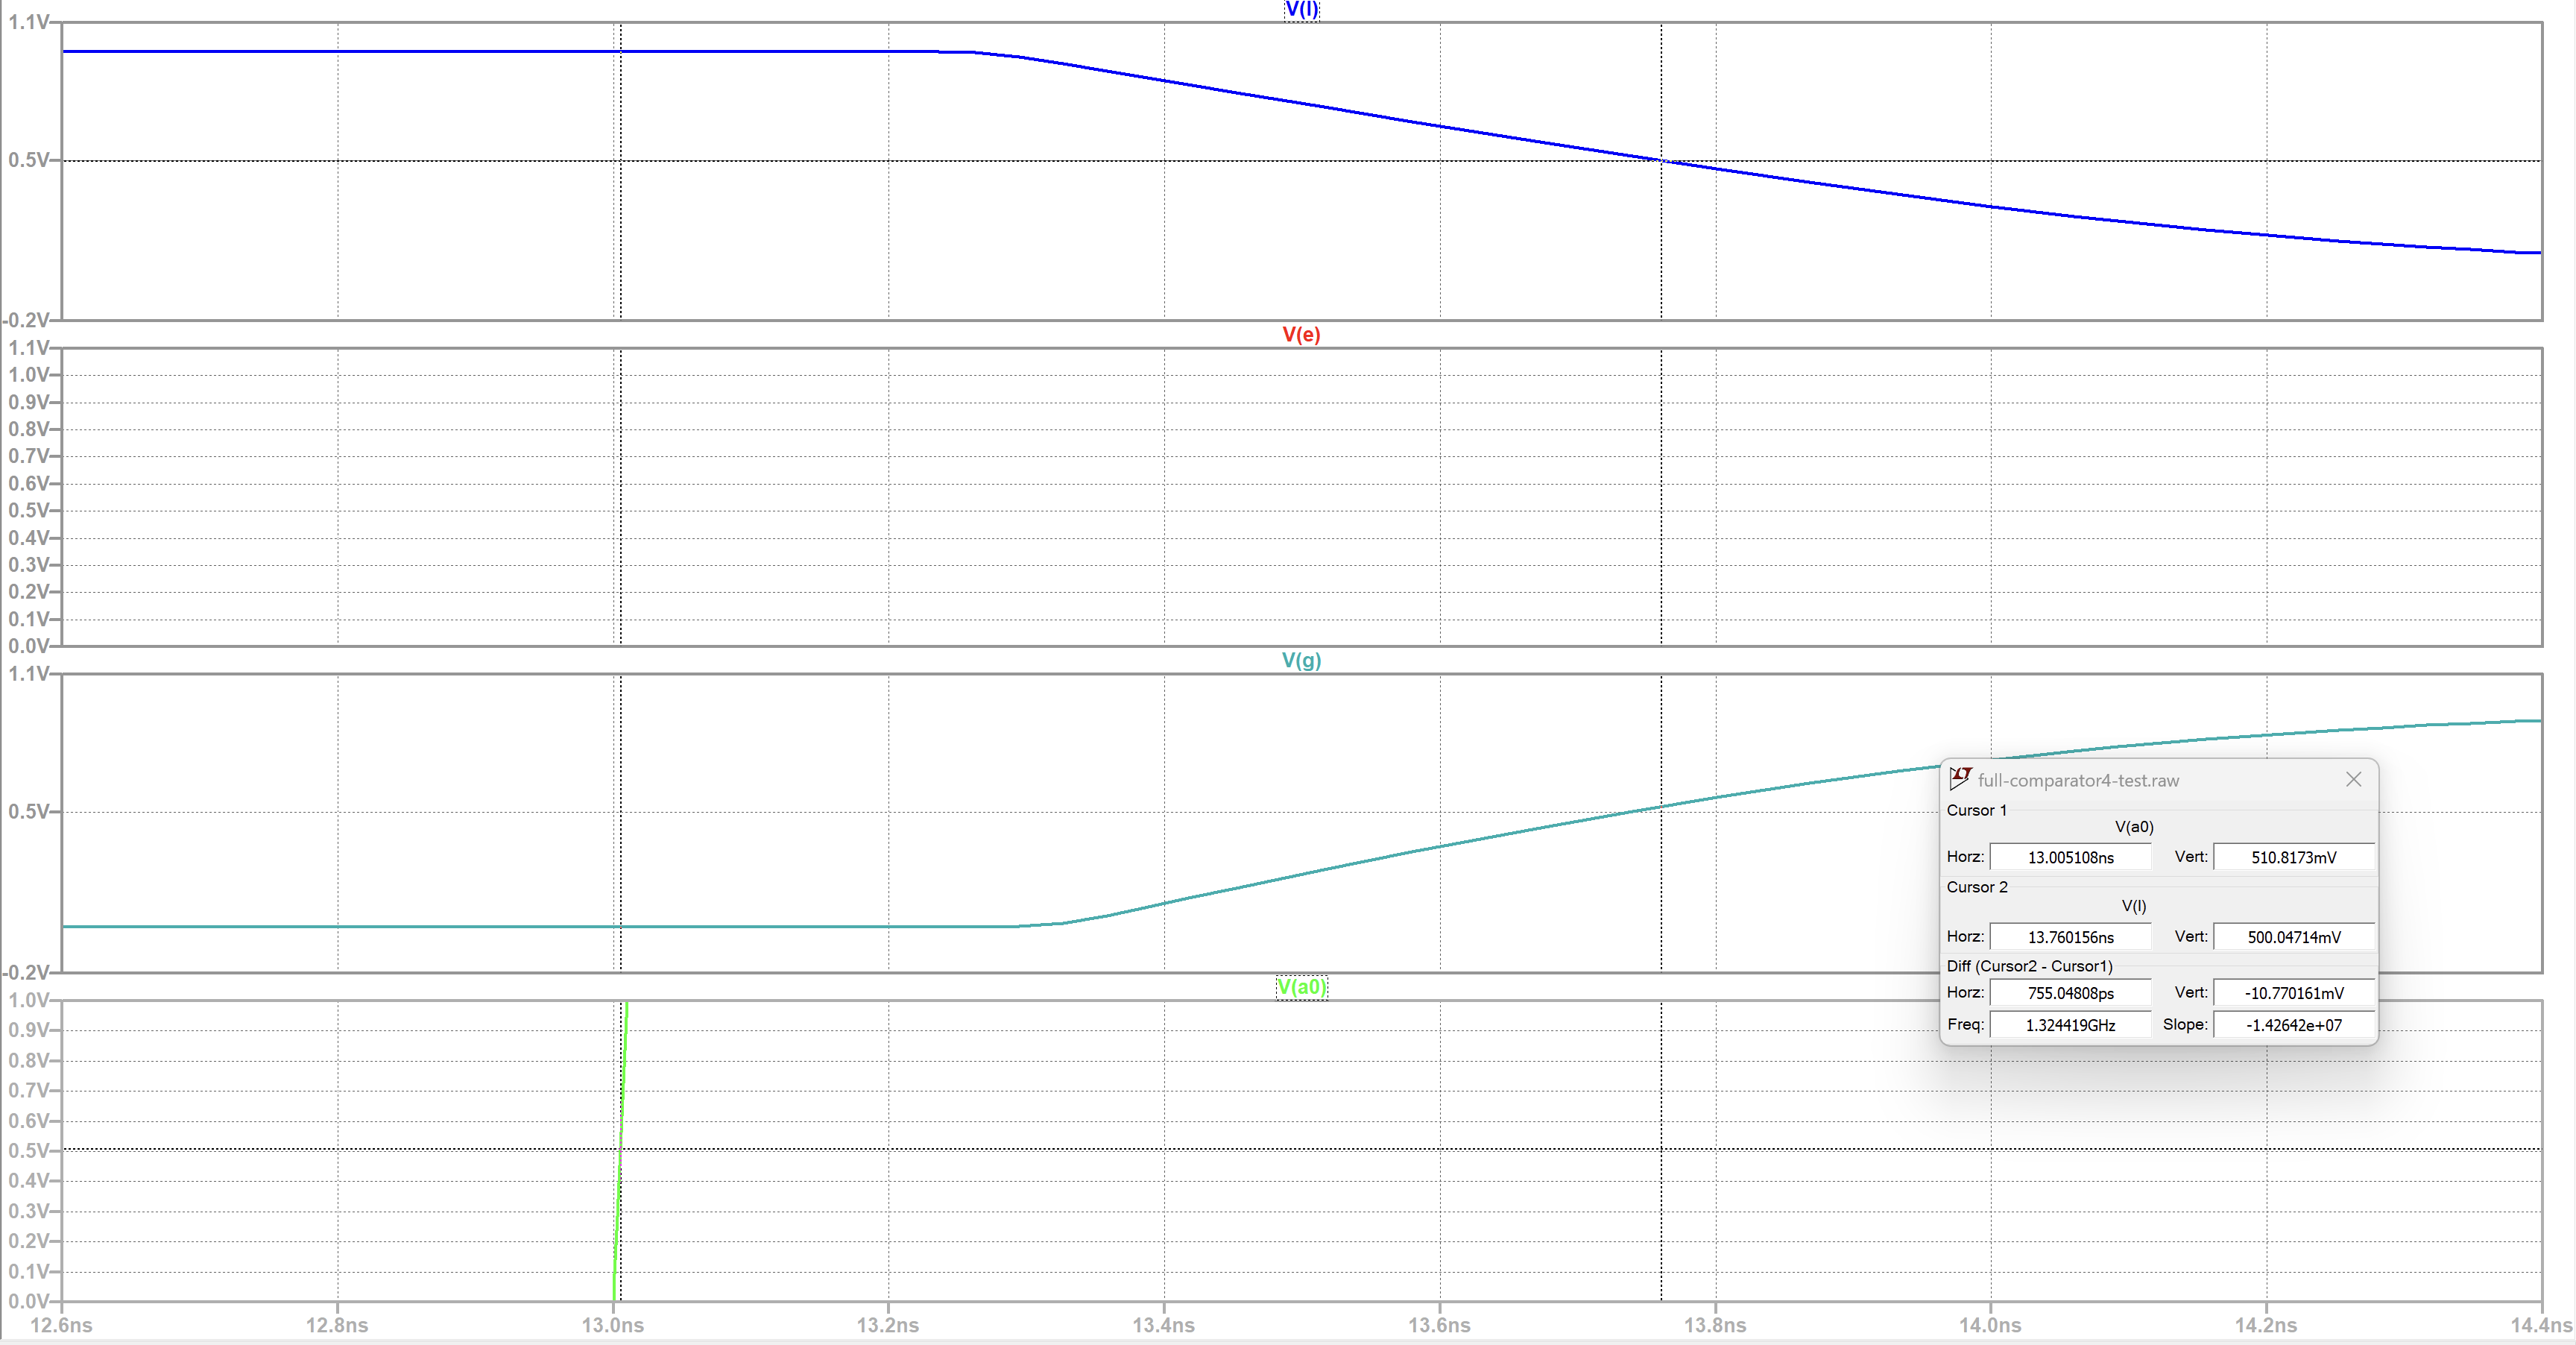
\includegraphics[width=\textwidth]{image/full-comparator-test-less-10.png}
    \caption{Подсчет задержки распространения сигнала для 1-0 на выходе less}
\end{figure}
$$t_{\text{pd}} = 13.760 - 13.005 = 0.755 ns$$
\begin{figure}[H]
    \centering
    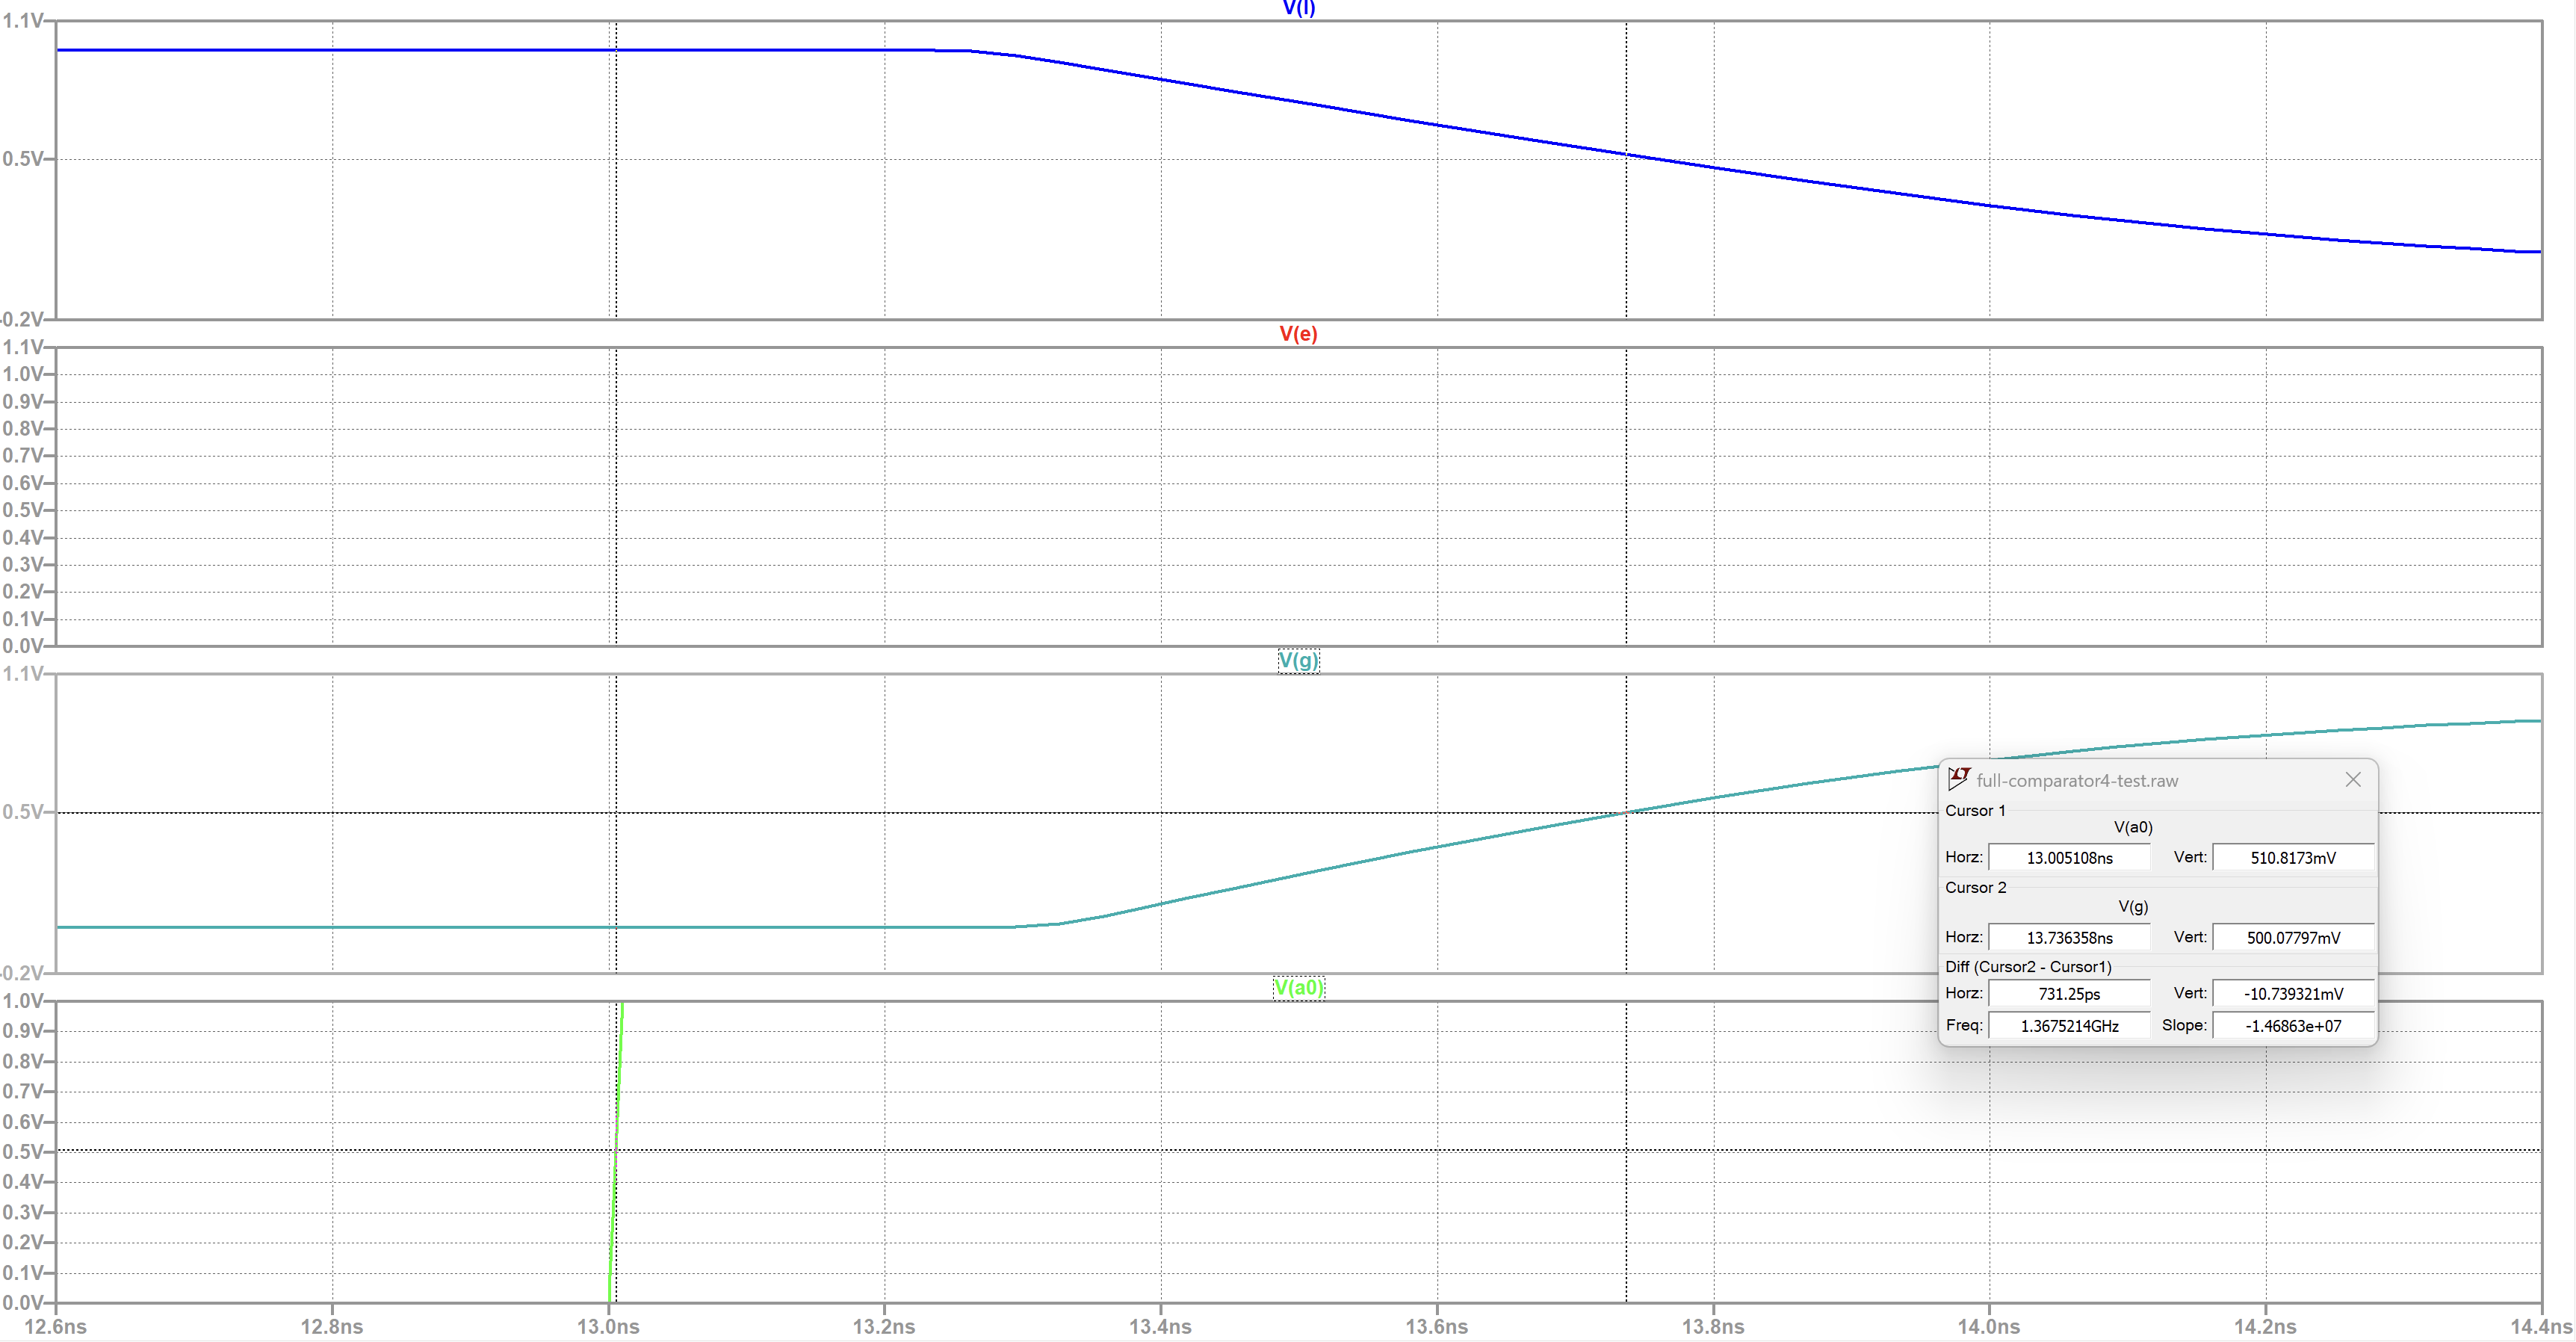
\includegraphics[width=\textwidth]{image/full-comparator-test-gt-01.png}
    \caption{Подсчет задержки распространения сигнала для 0-1 на выходе greater}
\end{figure}
$$t_{\text{pd}} = 13.736 - 13.005 = 0.731 ns$$
\begin{figure}[H]
    \centering
    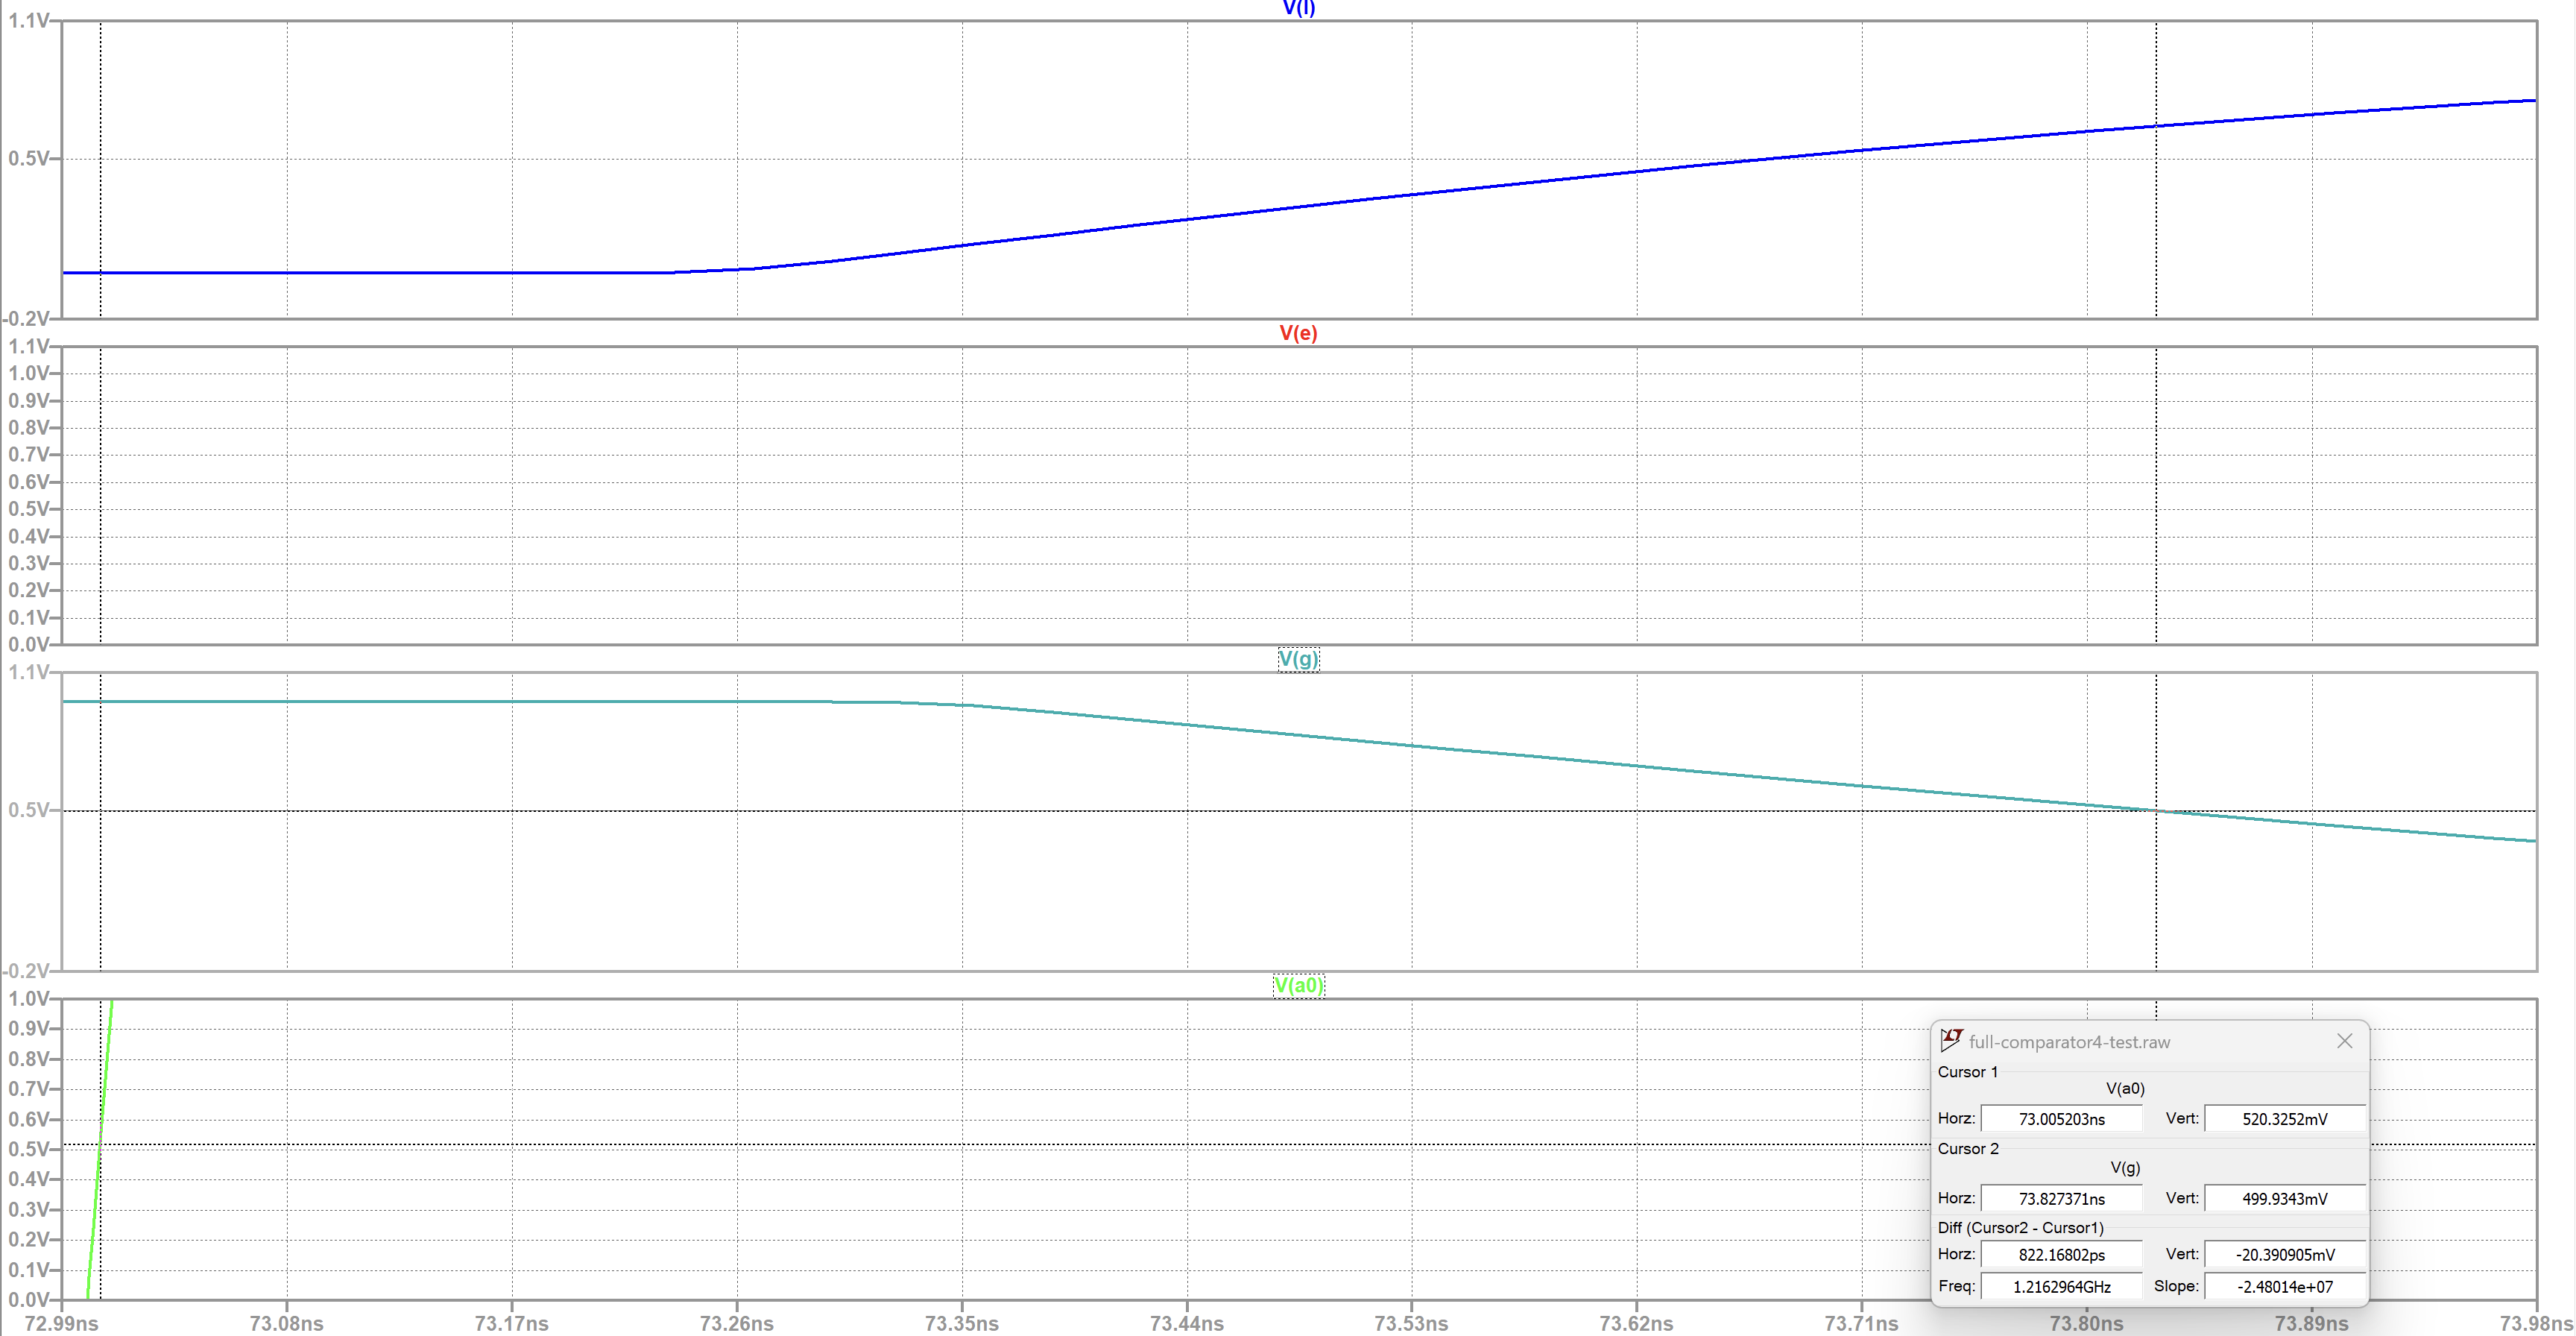
\includegraphics[width=\textwidth]{image/full-comparator-test-gt-10.png}
    \caption{Подсчет задержки распространения сигнала для 1-0 на выходе greater}
\end{figure}
$$t_{\text{pd}} = 73.827 - 73.005 = 0.822 ns$$
\subsection{Максимальная частота работы БОЭ.}
\begin{figure}[H]
    \centering
    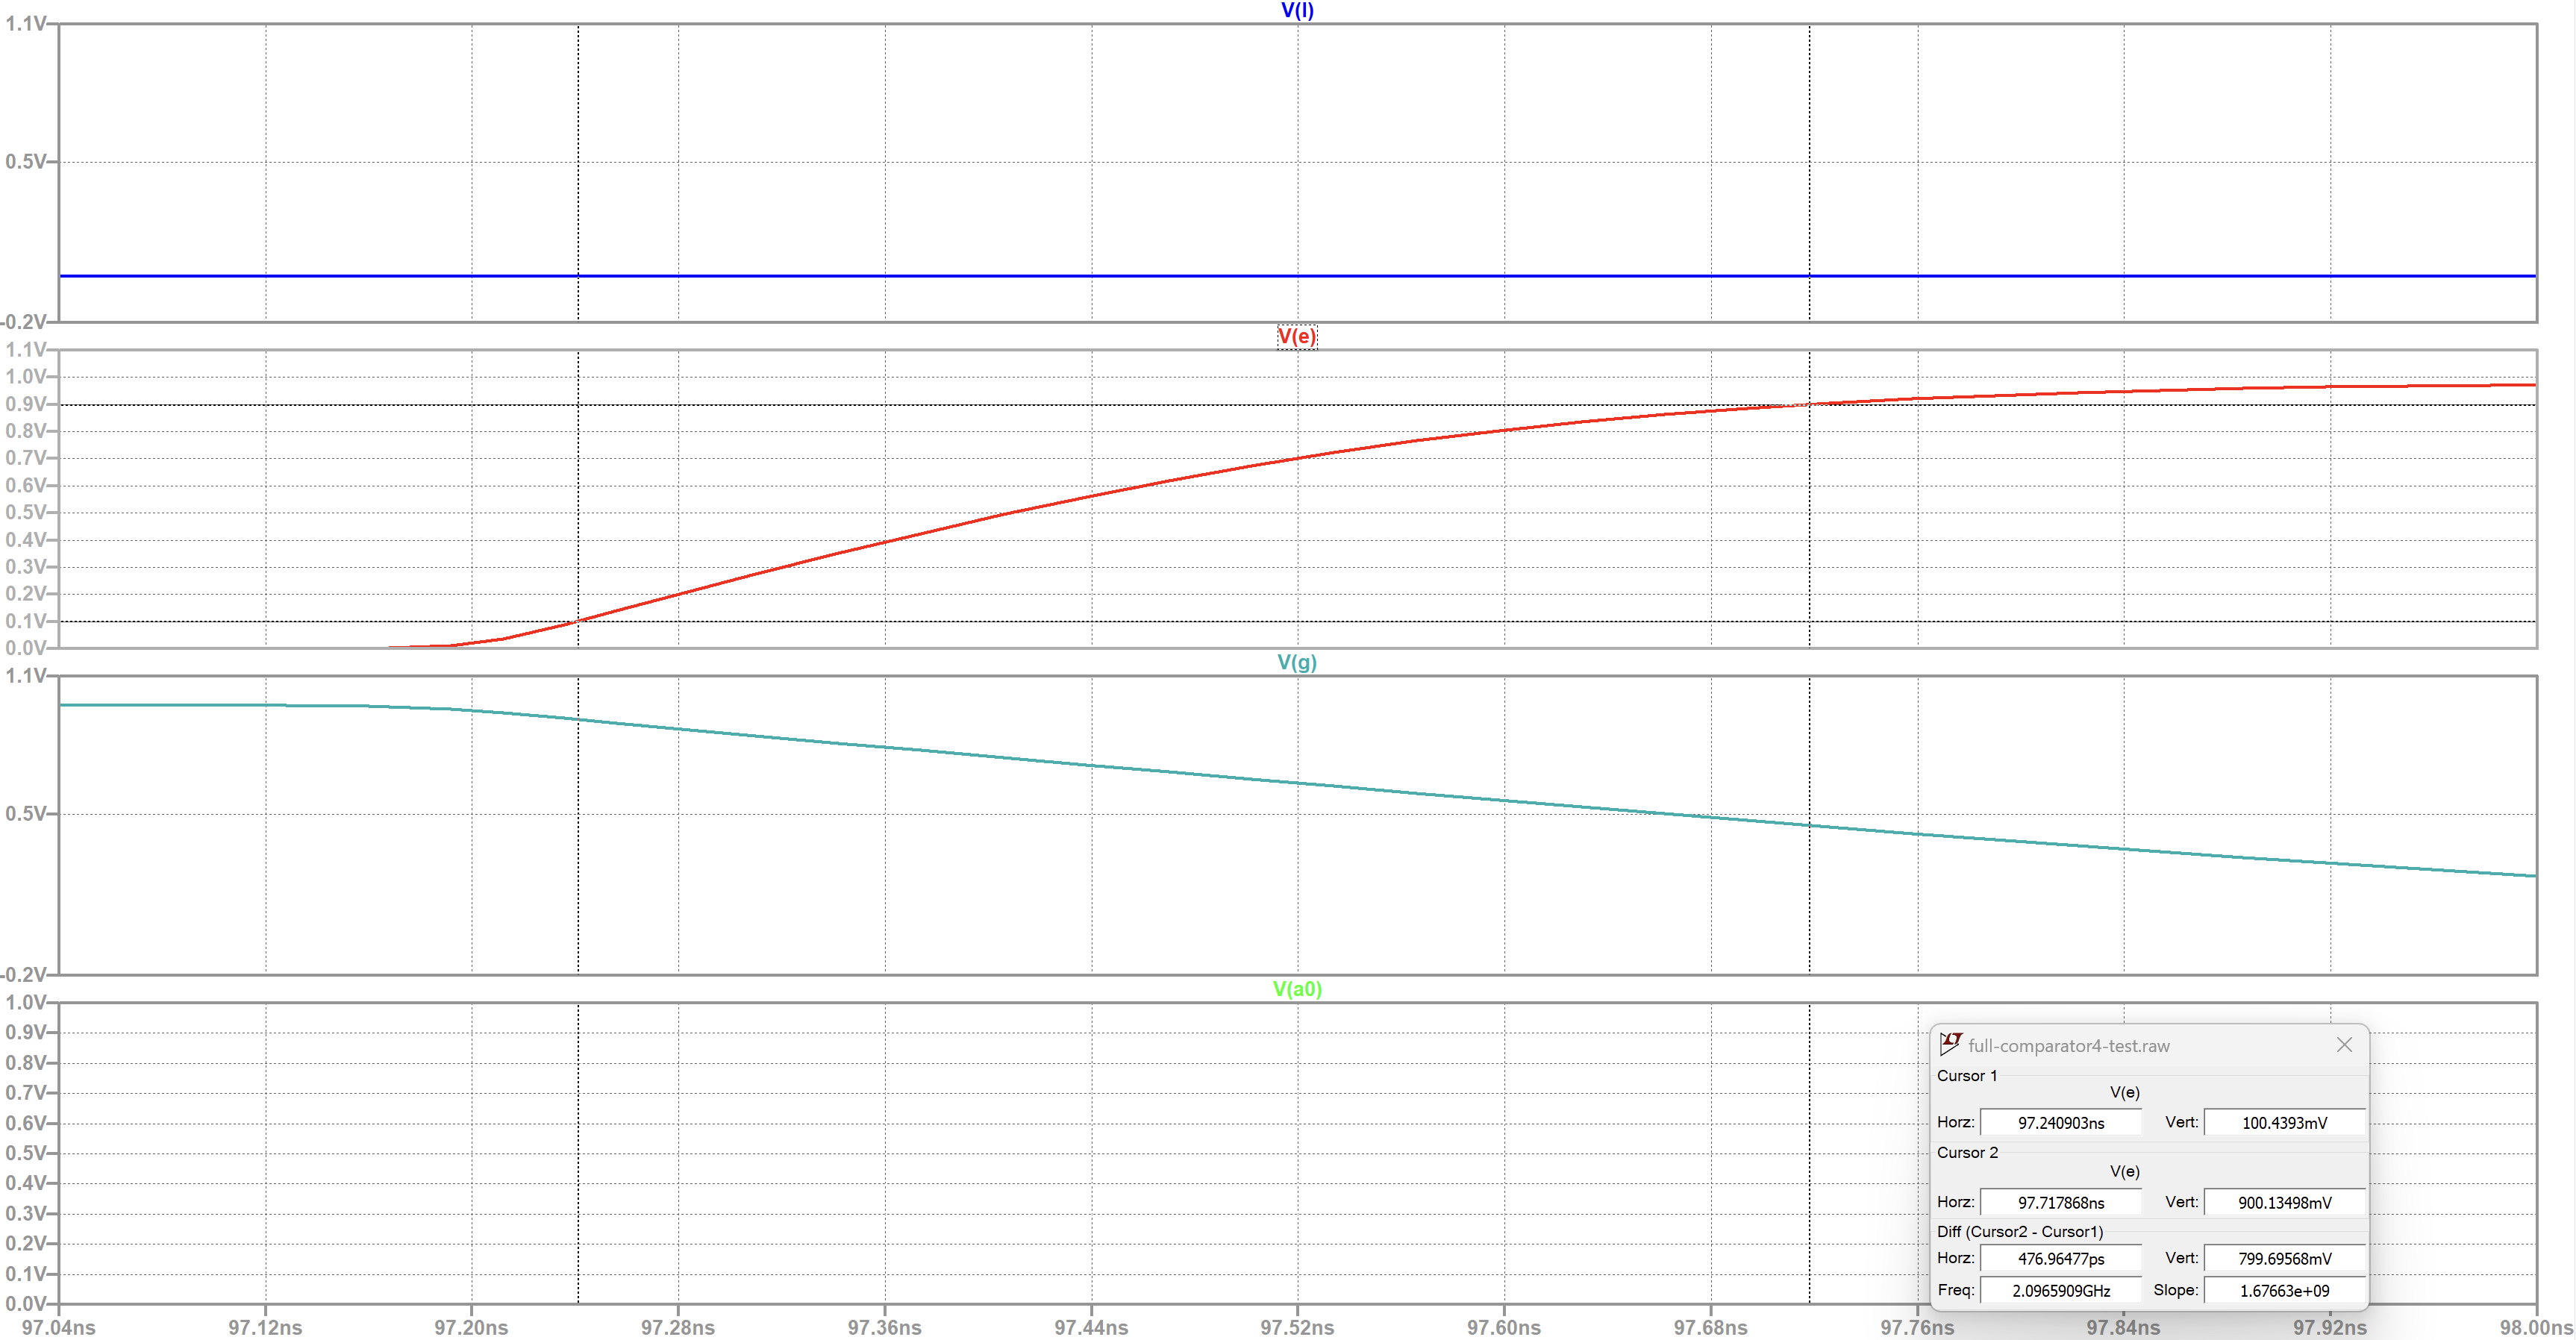
\includegraphics[width=\textwidth]{image/full-cmp-eq-freq-01.png}
    \caption{Время фронта от 0.9 до 0.1 для equal}
\end{figure}
$$ t_{\text{фронта}_{\text{eq}}}=97.718 - 97.241 = 0.477 ns$$
\begin{figure}[H]
    \centering
    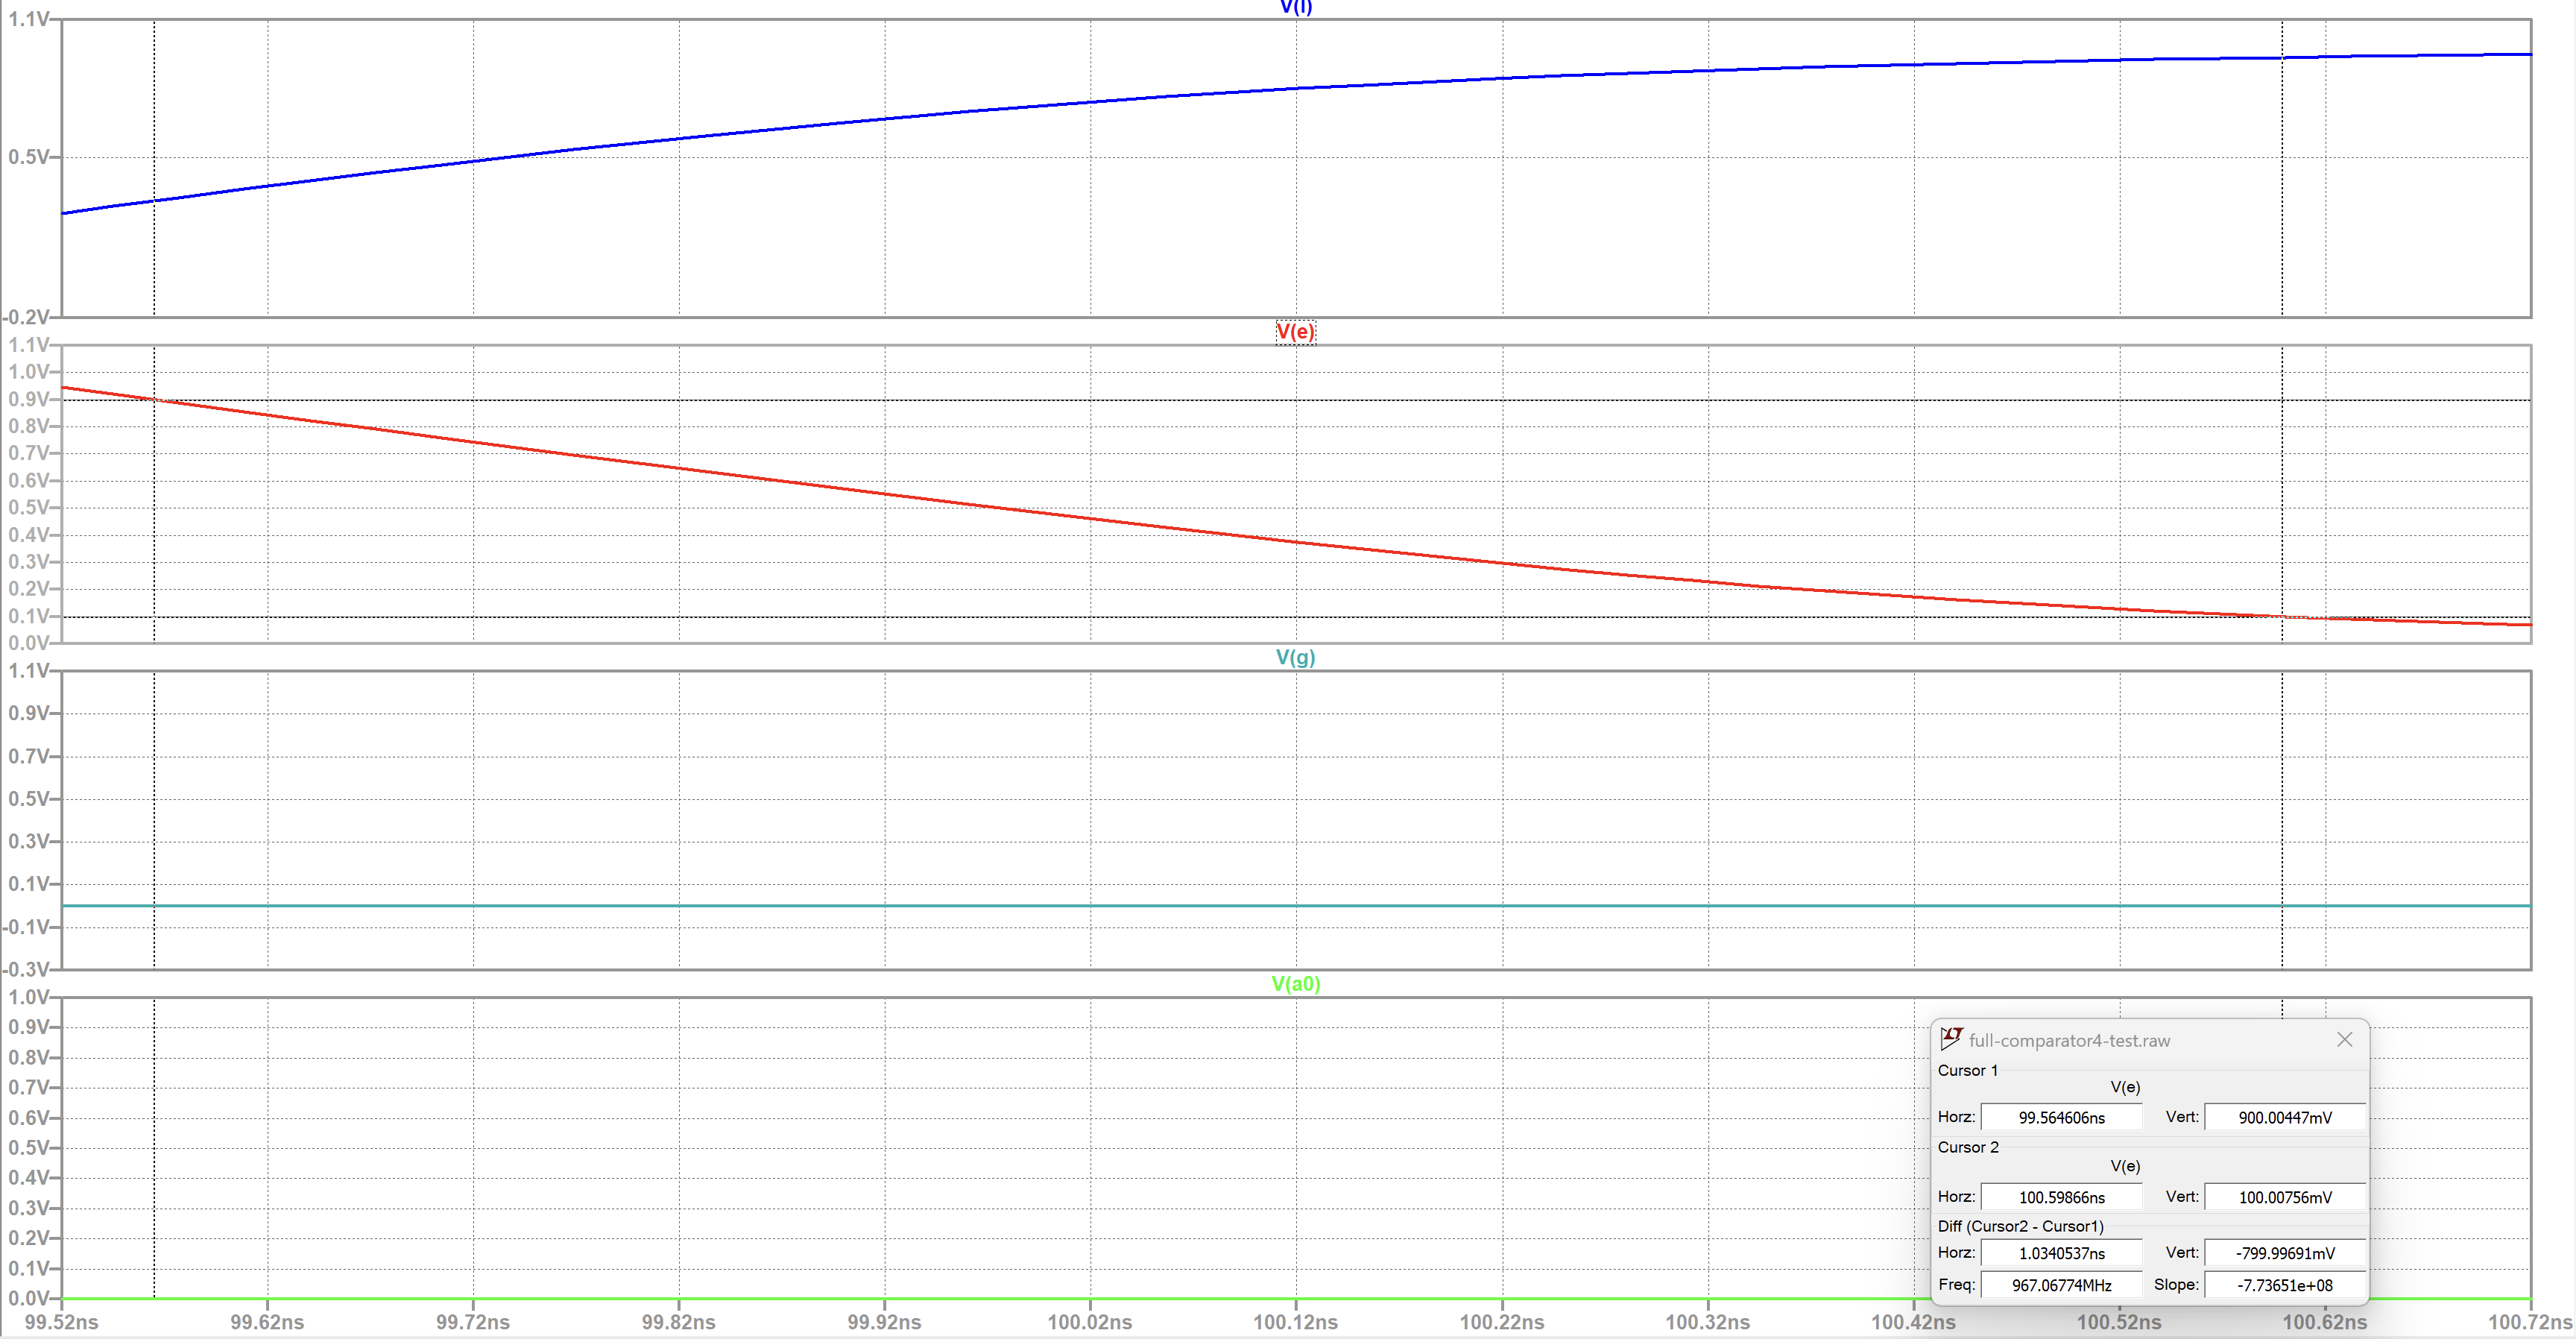
\includegraphics[width=\textwidth]{image/full-cmp-eq-freq-10.png}
    \caption{Время спада от 0.1 до 0.9 для equal}
\end{figure}
$$ t_{\text{спада}_{\text{eq}}}=100.599 - 99.565 = 1.034 ns$$
\begin{figure}{H}
    \centering
    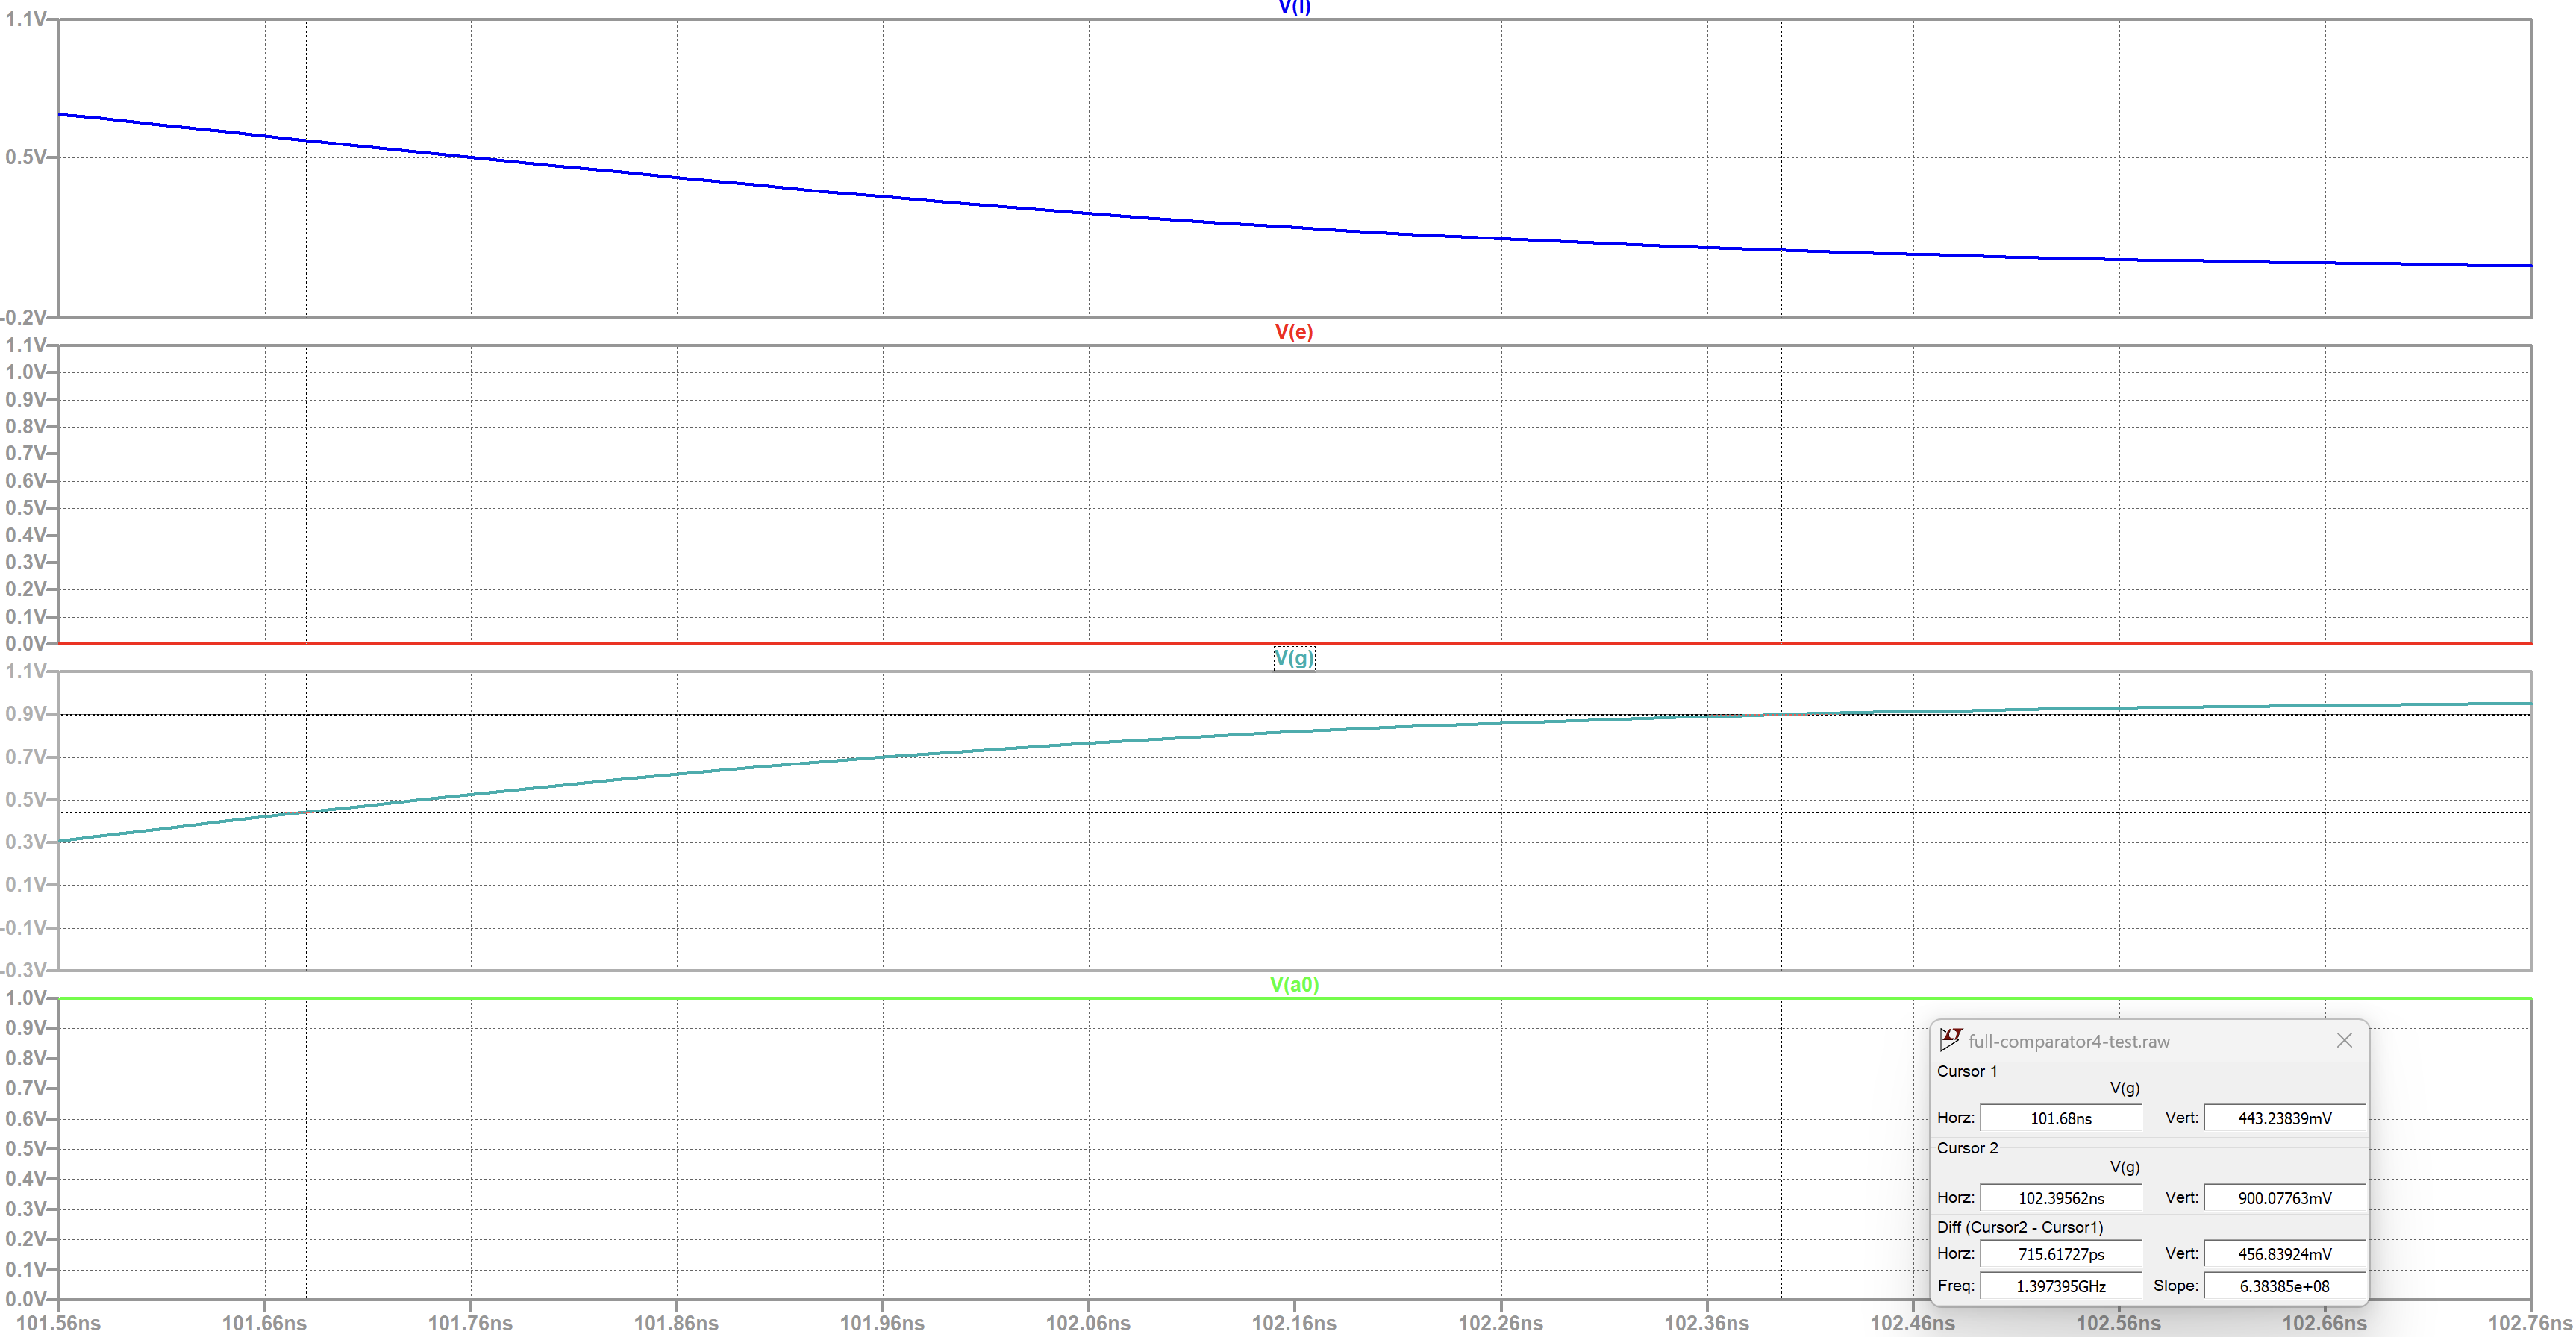
\includegraphics[width=\textwidth]{image/full-cmp-gt-freq-01.png}
    \caption{Время фронта от 0.9 до 0.1 для greater}
\end{figure}
$$ t_{\text{фронта}_{\text{gt}}}=102.396 - 101.68 = 0.716 ns$$
\begin{figure}{H}
    \centering
    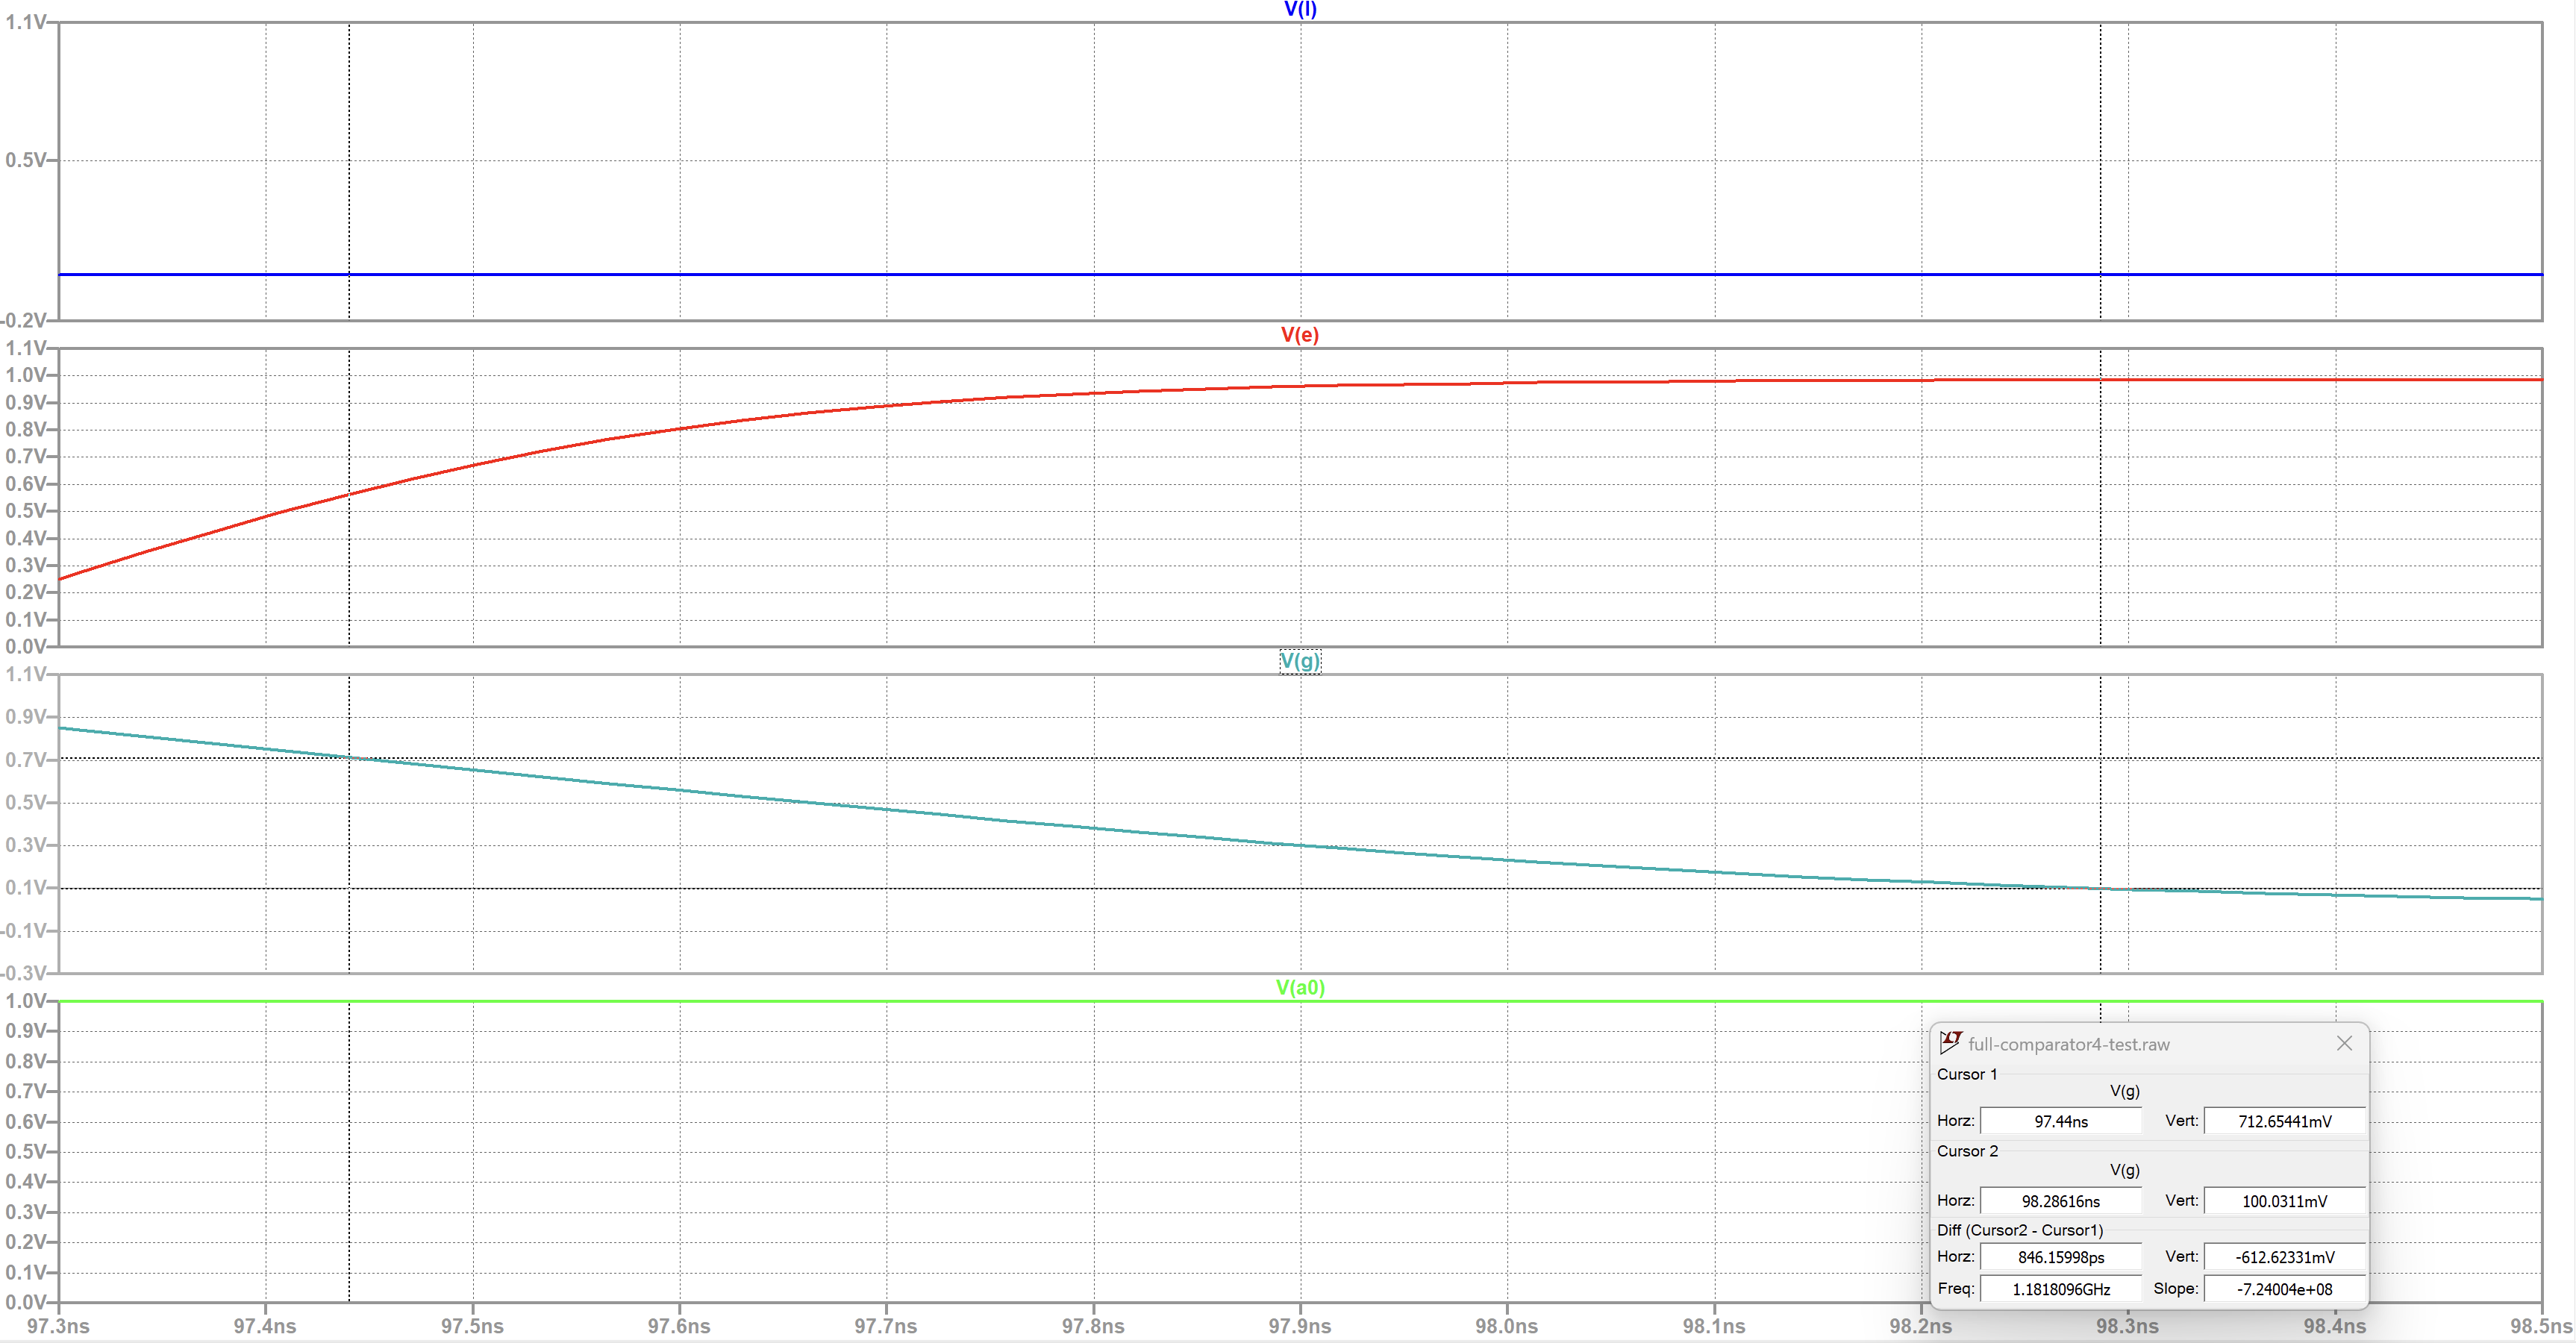
\includegraphics[width=\textwidth]{image/full-cmp-gt-freq-10.png}
    \caption{Время спада от 0.1 до 0.9 для greater}
\end{figure}
$$ t_{\text{спада}_{\text{gt}}}=98.286 - 97.44 = 0.846 ns$$
\begin{figure}[H]
    \centering
    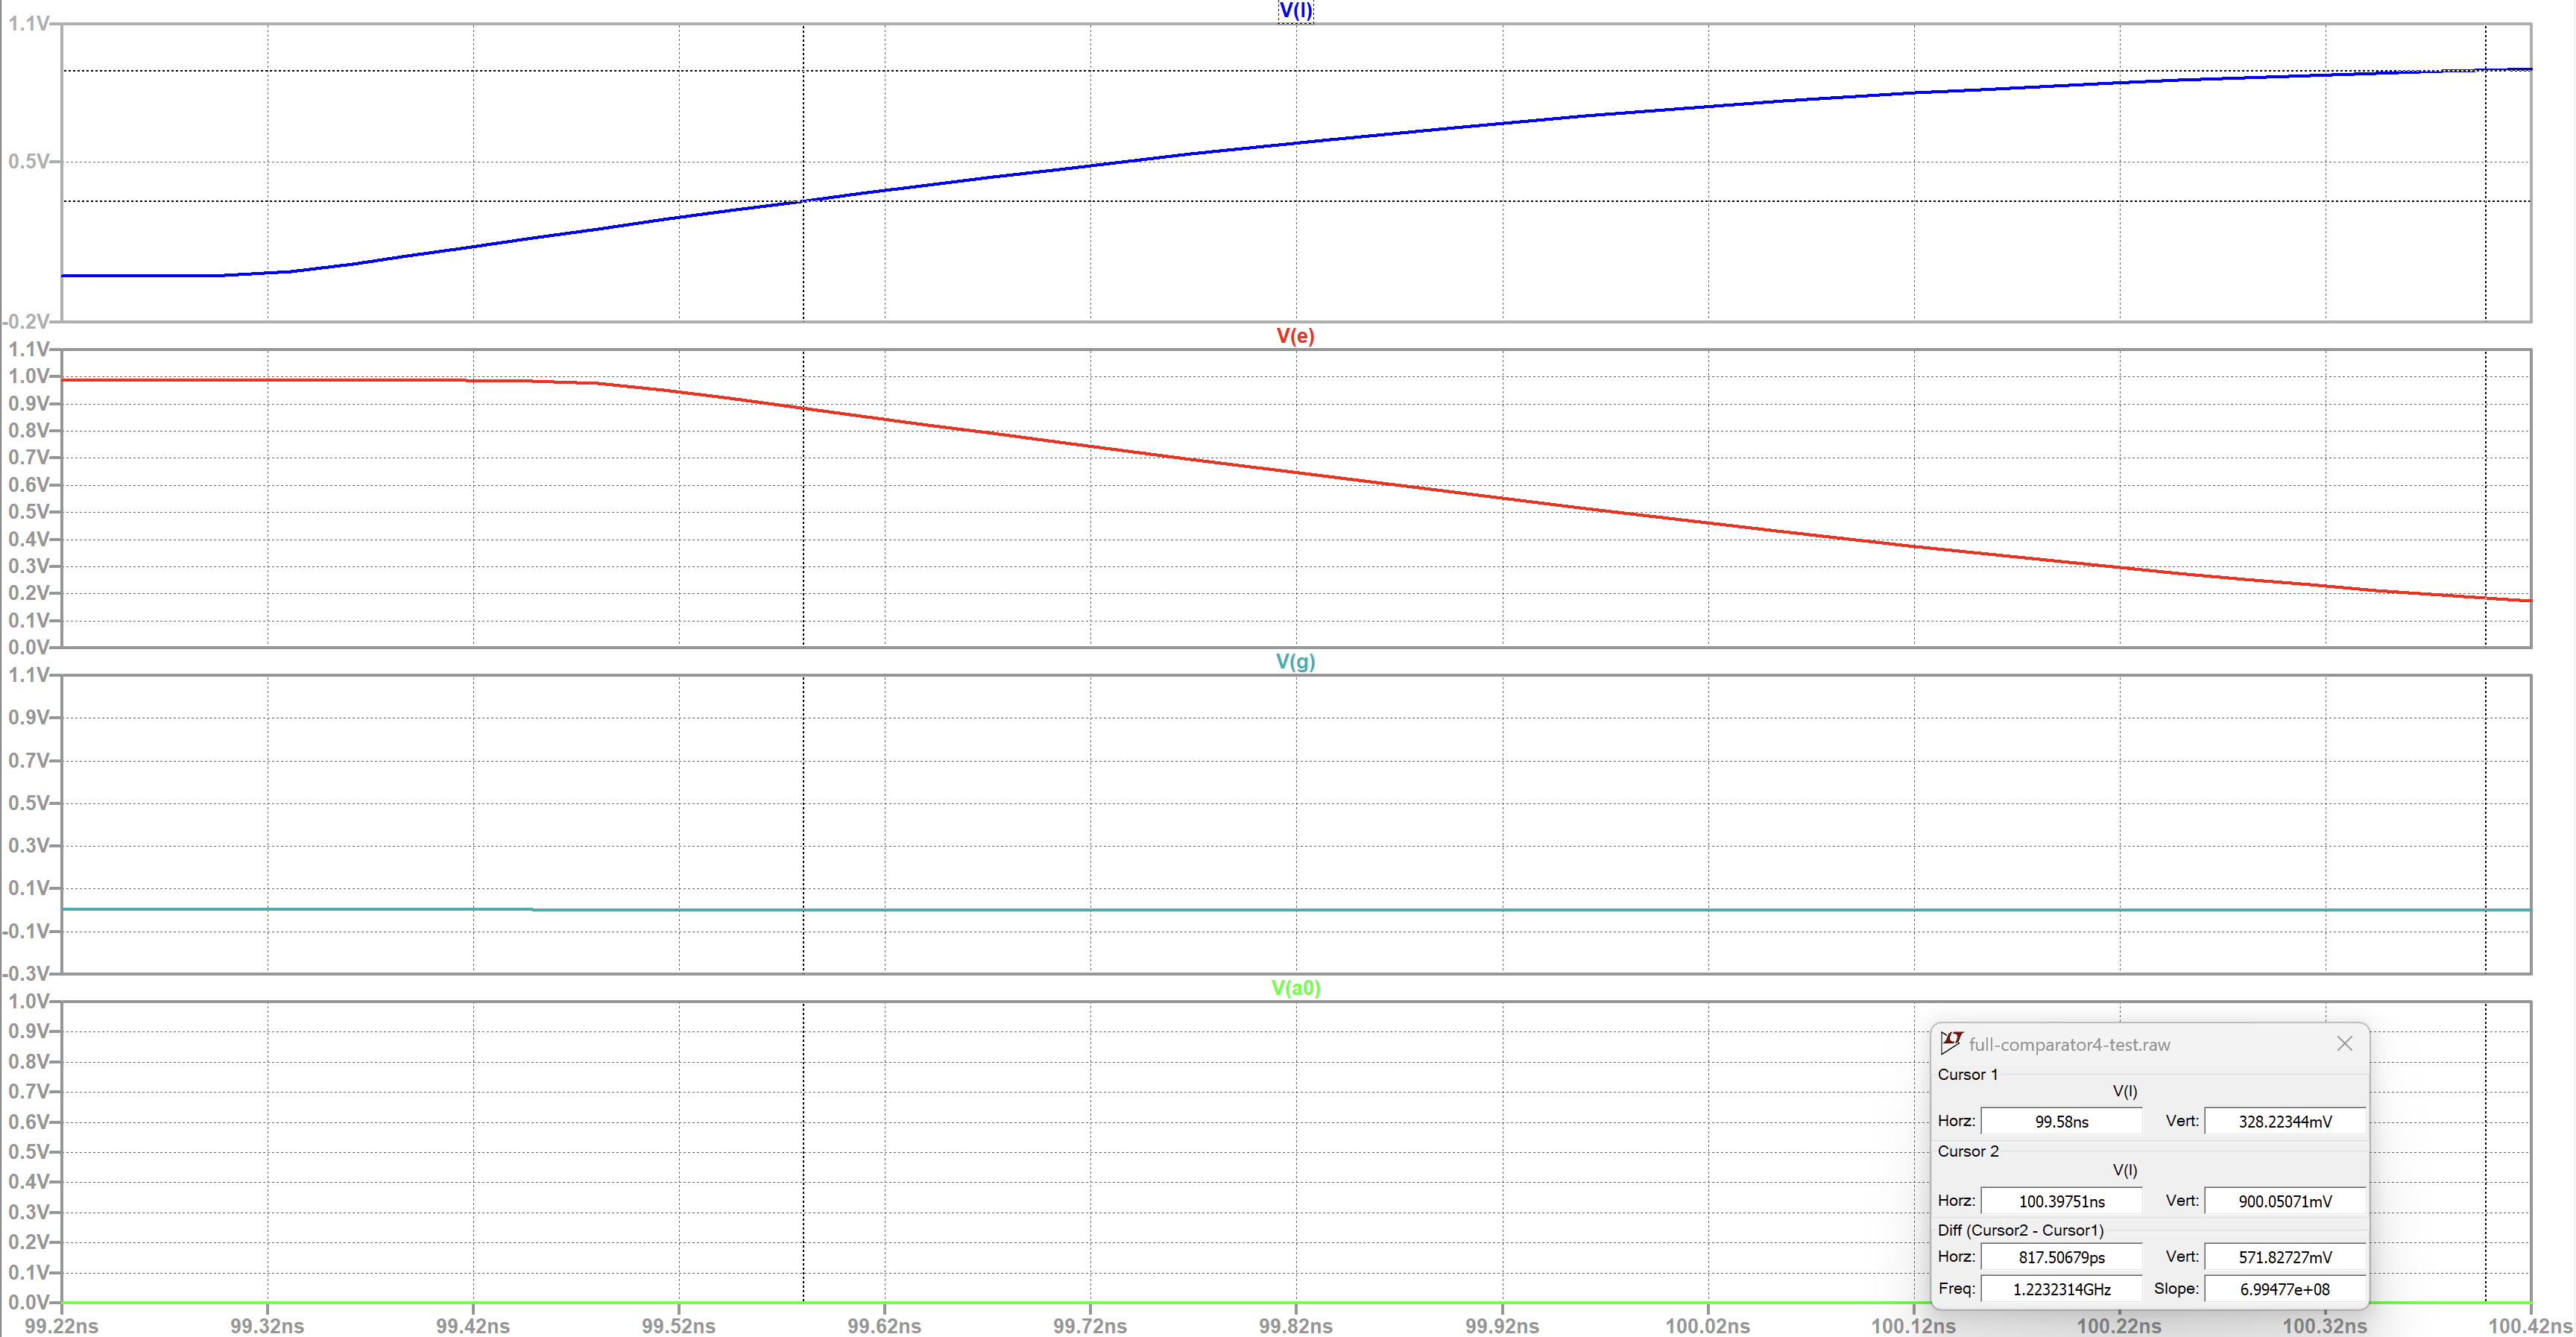
\includegraphics[width=\textwidth]{image/full-cmp-lt-freq-01.png}
    \caption{Время фронта от 0.9 до 0.1 для less}
\end{figure}
$$ t_{\text{фронта}_{\text{lt}}}=100.398 - 99.58 = 0.818 ns$$
\begin{figure}[H]
    \centering
    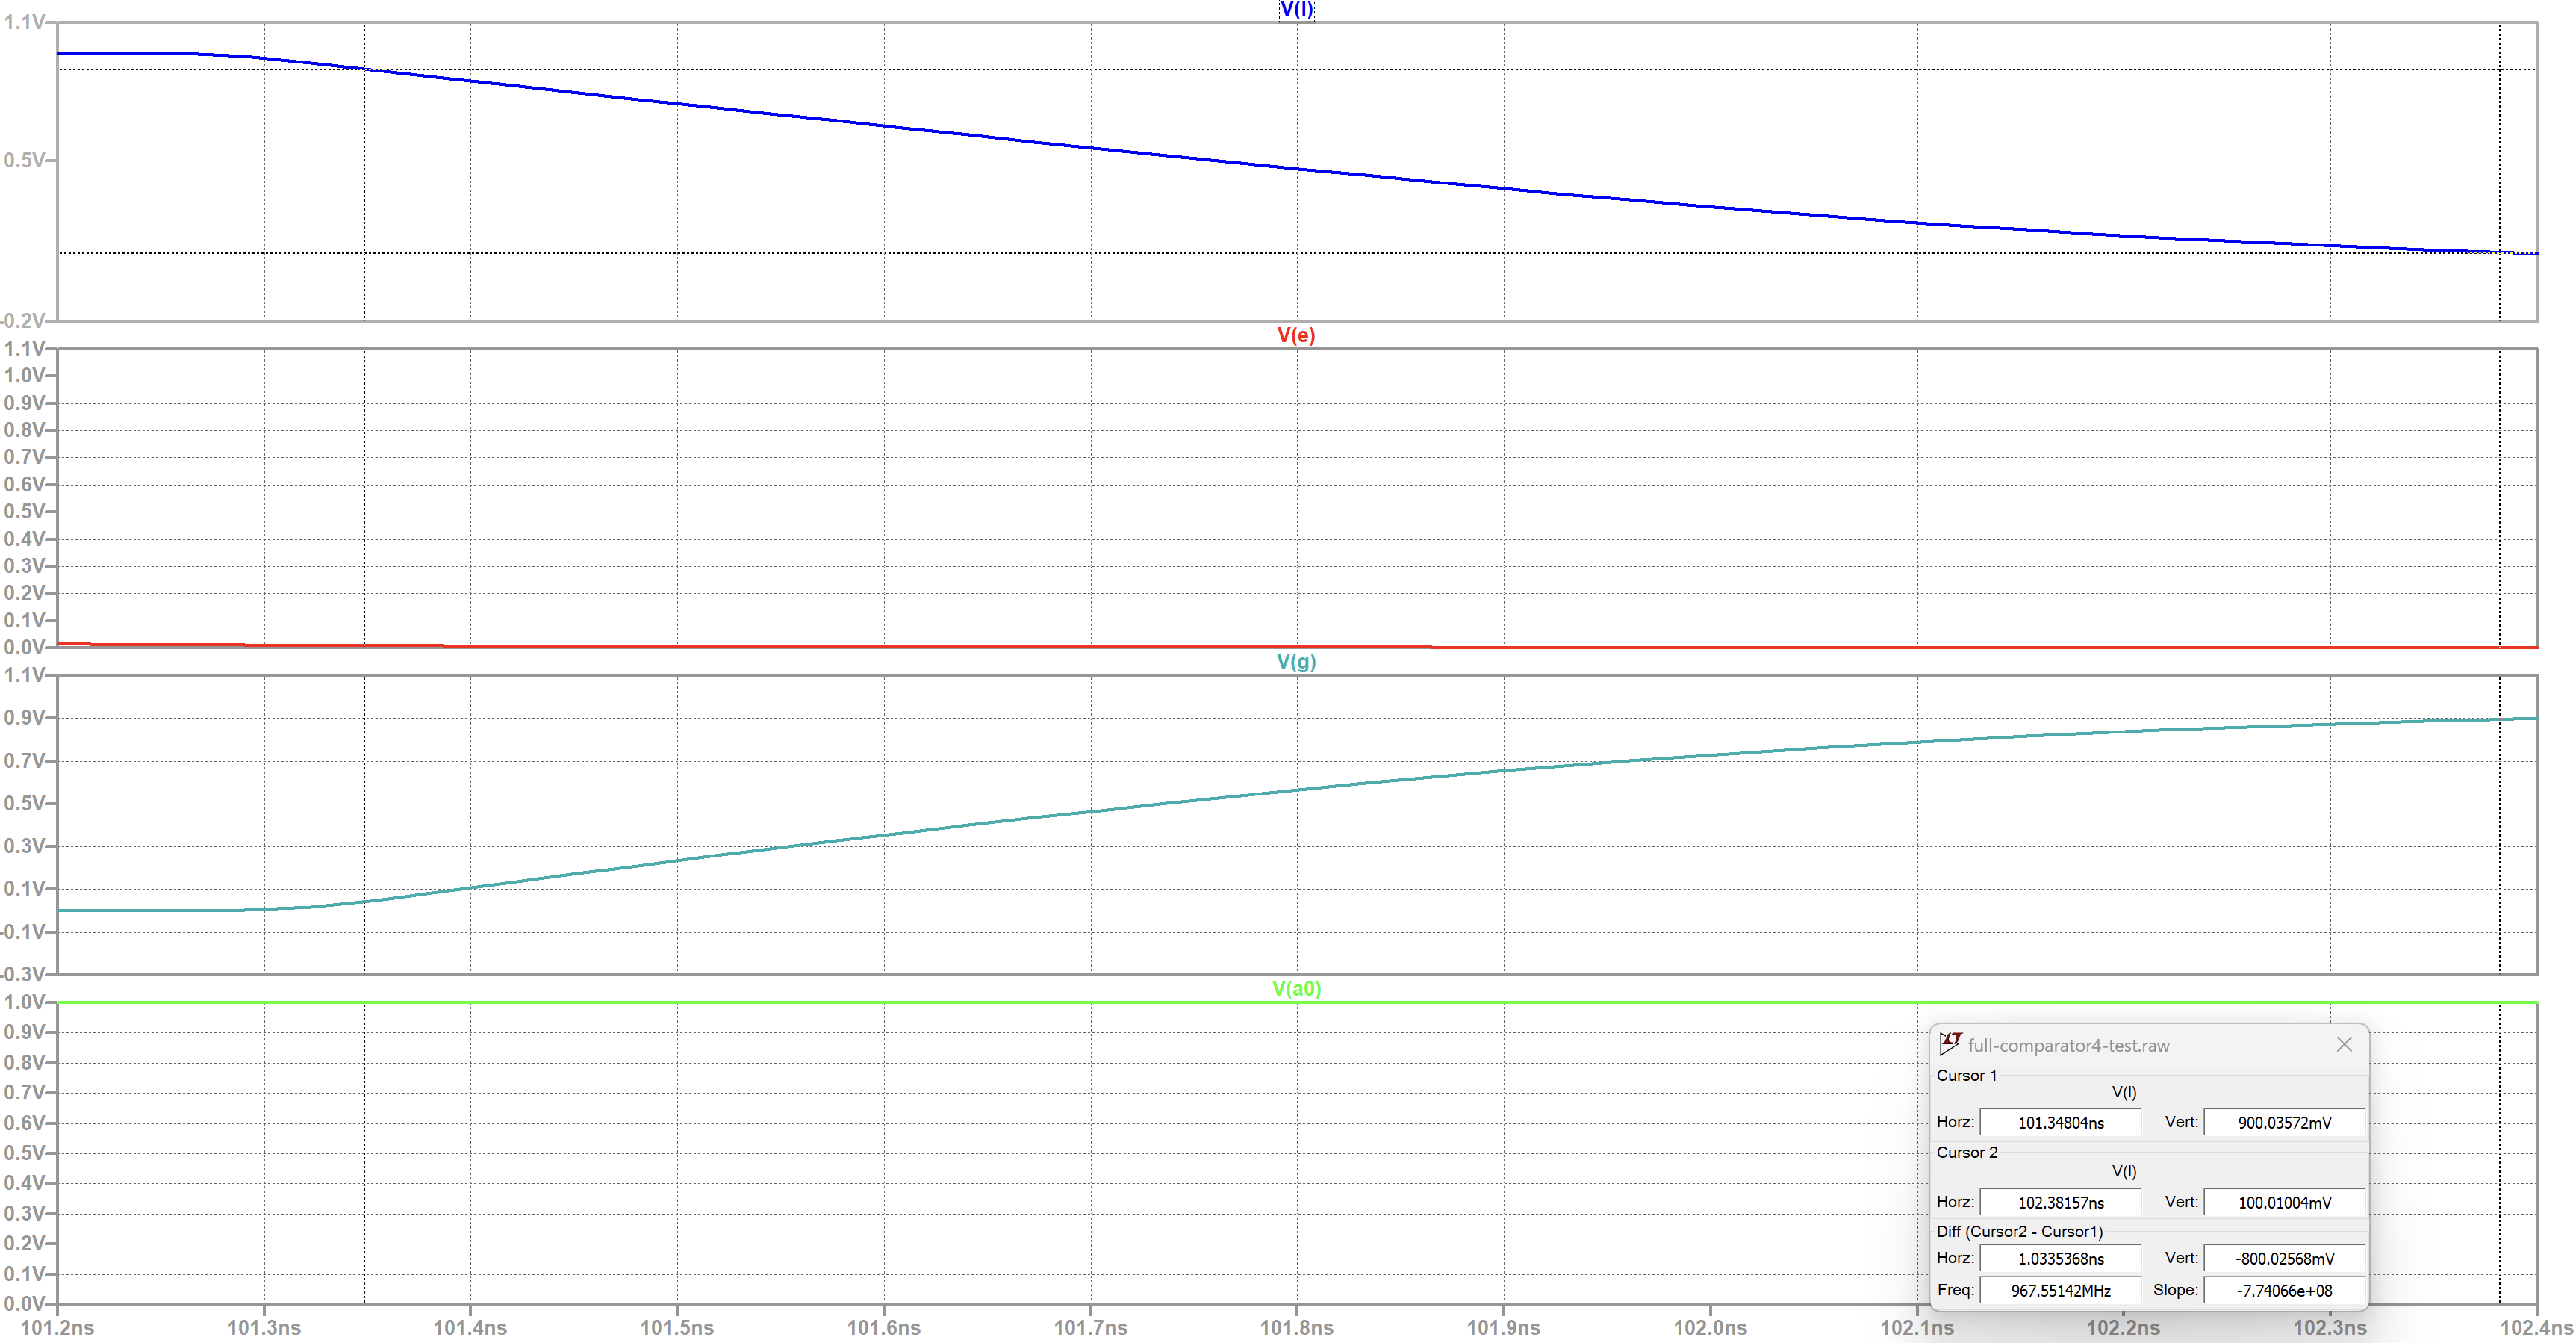
\includegraphics[width=\textwidth]{image/full-cmp-lt-freq-10.png}
    \caption{Время спада от 0.1 до 0.9 для less}
\end{figure}
$$ t_{\text{спада}_{\text{lt}}}=102.382 - 101.348 = 1.034 ns$$

Тогда максимальная частота схемы:
$$ \nu_{\max} = \frac{1}{\max(t)}= \frac{1}{1.034} = 0.967\text{ГГц}$$

\section{Отчет о выполнении заданий части 2:}
\subsection{Код разработанного модуля БОЭ}
\end{document}